\scanpage{1}
\begin{center}
{\Huge\sffamily IMAG}\\[1ex]
{\sffamily INSTITUT MONTPELLIERAIN}\\
{\sffamily ALEXANDER GROTHENDIECK}
\end{center}
\figure{
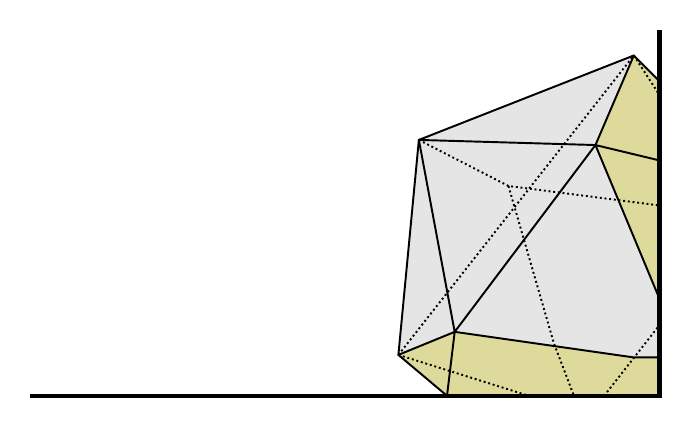
\begin{tikzpicture}[x=0.65cm,y=0.65cm,line width=.7pt]
\coordinate (A) at (0,0.8); \coordinate (B) at (.4,5);
\coordinate (C) at (4.6,6.65); \coordinate (D) at (5.1,6.15);
\coordinate (E) at (5.1,1.9); \coordinate (F) at (5.1,0);
\coordinate (G) at (.95,0); \coordinate (H) at (1.1,1.25);
\coordinate (I) at (3.85,4.9); \coordinate (J) at (2.15,4.1);
\fill[gray!20] (A)--(B)--(C)--(I)--(E)--(5.1,.75)--(4.6,.75)--(H)--cycle;
\fill[olive!30] (C)--(D)--(5.1,4.6)--(I)--cycle;
\fill[olive!30] (I)--(5.1,4.6)--(E)--cycle;
\fill[olive!30] (A)--(H)--(4.6,.75)--(5.1,.75)--(F)--(G)--cycle;
\draw (A)--(B)--(C)--(D)--(F)--(G)--cycle;
\draw (B)--(I)--(C) (I)--(5.1,4.6) (I)--(E);
\draw (B)--(H)--(G) (H)--(I) (A)--(H)--(4.6,.75)--(5.1,.75);
\draw[densely dotted] (A)--(C) (B)--(J)--(5.1,3.72);
\draw[densely dotted] (J)--(3.04,1.02)--(3.43,0);
\draw[densely dotted] (A)--(2.55,0) (C)--(5.1,5.88);
\draw[densely dotted] (4.02,0)--(5.1,1.38);
\draw[line width=1.6pt] (-7.2,0)--(5.1,0)--(5.1,7.15);
\end{tikzpicture}
}

\scanpage{2}
\margin{19 pages}
Catégories de \unsure{Galois-Teichmüller|Galois Teichmüller}
d'un corps alg. clos.

\margin{1}

\scanpage{3}
\mspage{1}
Soient $X$ et $Y$ deux surfaces topologiques orientées \inserted{(connexes pour simplifier)} ``de type fini'' (i.e. déduites de surfaces compactes en enlevant un nb fini de points). On considère
\[
\begin{aligned}
(1)\qquad \operatorname{Hom}_{\mathrm{isot}}(X,Y)
&=\text{ensemble des composantes connexes \inserted{par arcs}}\\
&\quad\text{de l'espace des applications finies}\\
&\quad\text{étales de $X$ dans $Y$ \deleted{respectant}}\\
&\quad\deleted{\text{l'orientation}}
\end{aligned}
\]
Si $f$ et $g$ sont deux applications finies étales de $X$ dans $Y$, alors $f$ et $g$ \inserted{sont isotopes i.e.} définissent la $=$ \deleted{\unsure{appli}} application de $X$ en $Y$ dans la cat. isotopique, ssi nous pouvons trouver une application continue \unsure{fin étal|fin ét}
\deleted{$F$ de $X\times I$}
\[
(2)\qquad F:X\times I\longrightarrow Y\times I\qquad I=[0,1]
\]
commutant aux projections sur $I$, et telle que
\[
(3)\qquad F(x,0)=(f(x),0)\qquad F(x,1)=(g(x),1)\qquad\forall x\in X
\]
Comme le foncteur
\[
Y'\longmapsto Y'\times I
\]
des rev. finis étales de $Y$ vers les rev. finis étales de $Y\times I$ est pl. fidèle, on voit que \deleted{\unsure{il exi}} pour $F$ donné, il doit exister un rev. fini étale $Y'$ de $Y$, unique à isom. unique près, et une \unsure{homéom.}
\[
(4)\qquad \alpha:X\times I\xrightarrow{\sim}Y'\times I
\]
rendant commutatif le diag. \unsure{comm.|suiv.}
\diagram{
\begin{tikzcd}[ampersand replacement=\&]
(5)\quad X\times I \arrow[rr,"\alpha", "\sim"'] \arrow[dr,"F"'] \&\& Y'\times I \arrow[dl,"p\times\operatorname{id}_I"]\\
\&Y\times I\&
\end{tikzcd}
}
\margin{où $p:Y'\longrightarrow Y$ la projection}
\margin{2}

\scanpage{4}
En d'autres termes, on a $f\overset{\mathrm{isot.}}{\sim}g$ ssi il existe un rev. \inserted{fini} étale (unique à isom. unique près) $Y'$ de $Y$, de telle façon que l'on ait
\[
(6)\qquad f=pf_0,\qquad g=pg_0
\]
\margin{$p:Y'\mathbin{-}Y$ la projection}
où
\[
(7)\qquad f_0:X\xrightarrow{\sim}Y'\qquad g_0:X\simeq Y'
\]
sont des homéomorphismes de $X$ en $Y'$ qui sont \unsure{isotopes|homotopes}, ou ce qui revient au $=$, tels que l'on ait
\[
(8)\qquad g_0=f_0\circ u
\]
où
\[
(9)\qquad u:X\xrightarrow{\sim}X
\]
\unsure{où} est un homéom. de $X$ sur lui $=$ isot. à l'identité. On aura donc, par (6) et (8),
\[
g=pg_0=p(f_0\circ u)=(pf_0)u=f\circ u
\]
Donc on trouve

\uline{Proposition 1} Pour que deux \deleted{applications} \inserted{morphismes} fini\deleted{\unsure{e}}s étales $f,g:X\longrightarrow Y$ soient isotopes, il f. et s. qu'ils soient \unsure{congrus|conjugués} sous le groupe des autom. de $X$ isotopes à l'identité; i.e $g=fu$, où $u$ autom. de $X$ isotope à l'identité.

Soit un \deleted{\unsure{donné}} morphisme $f:X\longrightarrow Y$ dans la catégorie isotopique (1), peut-on le
\margin{3}

\scanpage{5}
\mspage{2}
(ce qui est \unsure{sans doute|loin d'être} tjs vrai, et \deleted{\unsure{dans}} \unsure{le critère} d'une \unsure{vraie conjugaison} de $\sigma$) on est ramené au cas précédent, en \deleted{enlevant} remplaçant $Y'$ par $Y'\setminus S'$, où $S'$ est l'ens. fini des pts de ramification pour l'action de $\sigma$. \deleted{\unsure{$E$}}

On fera attention que la \deleted{condition} \inserted{propriété} envisagée \deleted{n'est pas} (sur les autom. d'ordre fini de la surface $Y'$) n'est pas vérifiée sans restrictions. Si p.ex. $Y'=\mathbb{C}^*$, ou $Y'=\unsure{\mathbb{U}\times\mathbb{U}}$ alors les translations par des points d'ordre fini sont isotopes à l'identité, sans être néc. \unsure{égaux|égales} à l'identité ! Mais on a ceci
\figure{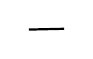
\begin{tikzpicture}[baseline=0pt]\draw[line width=.8pt] (0,0)--(.45,.01);\end{tikzpicture}}

\uline{Proposition 2} Soit $Y'$ une surface orientée de t.f. (\inserted{surf.} cpte $-$ nb fini de pts) \uline{anabélienne}, i.e. telle que pour tte comp. connexe $Y'_i$ de $Y'$, on ait $\chi_!(Y'_i)<0$ (i.e. on ait $2g_i+\nu_i\geq 3$, où $g_i$ est le genre de $Y'_i$ et $\nu_i$ le nb des trous\ldots). Alors tout autom. \inserted{$\sigma$} d'ordre fini de $Y'_i$ qui est isotope à l'identité est l'identité.

Comme $\sigma$ \unsure{respecte} les composantes connexes, OPS $Y'$ connexe. En fait, il suffit que $\sigma$ opère trivialement sur la homologie \inserted{$\unsure{H_1}$, \unsure{propre}} (à coefficients dans $\mathbb{Z}$, ou dans \inserted{\unsure{un}} $\mathbb{Z}/n\mathbb{Z}$ avec $n\geq3$) pour
\margin{4}

\scanpage{6}
factoriser \uline{canoniquement} en
\diagram{
\begin{tikzcd}[ampersand replacement=\&]
(10)\quad X \arrow[r,"f_0","\sim"'] \& Y' \arrow[r,"p"] \& Y
\end{tikzcd}
}
où $Y'$ est un rev. étale fini de $Y$, défini à isom. unique près, et où $X\xrightarrow{\sim}Y'$ est un isom dans la cat. isotopique -- i.e. une classe d'isotopie d'homéomorphismes ? Bien sûr, si on n'a pas \unsure{une d'exigence|une exigence} de canonicité, la factorisabilité (10) de $f$ est triviale -- il suffit de prendre un représentant quelconque de $f$. \deleted{\unsure{Plus|Pour}} Pour préciser la \deleted{question} condition d'unicité, on est amené à se poser la question si pour tt $Y$-autom. \deleted{$\unsure{g}$} $\sigma$ de $Y'$ \deleted{\unsure{la classe}} (\uline{pas} à isot. près !) \deleted{tel que l'on ait} on a l'implicat°
\[
(11)\qquad (\sigma f_0\sim\deleted{\unsure{\sigma}}f_0)\Longrightarrow\sigma=\operatorname{id}_{Y'}\quad ?
\]
Dans cette question, on peut bien sûr supposer $f_0=\operatorname{id}$, donc la question est si un autom d'ordre fini \inserted{$\sigma$} d'\deleted{une} \inserted{la} surface orientée $Y'$ de type fini, qui est isotope à l'identité, est l'identité.

La condition supplémentaire, que $\sigma$ est un $Y$-autom., où $Y'\unsure{-|\longrightarrow}Y$ est fini étale, signifie aussi que $\sigma$ opère via une opération \uline{libre} de $\mathbb{Z}/n\mathbb{Z}$ (où $n$ est l'ordre de $\sigma$) -- mais en admettant que si $\sigma$ \inserted{(autom. d'ordre fini)} n'est pas l'identité, ses pts fixes sont isolés,
\margin{5}

\scanpage{7}
\mspage{3}
que $\sigma$ soit l'identité. Pour le voir, on peut supposer que $\sigma$ laisse invariante une structure \deleted{\unsure{de}} de courbe algébrique (de type $(g,\nu)$ anabélien) sur $X$. Il suffit \deleted{\unsure{de}} que l'on ait $\unsure{2g-\nu\geq2|2g+\nu\geq2}$, i.e. que $X$ se plonge dans \unsure{sa} jacobienne généralisée, ext. d'une VA par un tore, pour pouvoir conclure de l'hypothèse homologique que $\sigma$ \deleted{est} induit une \uline{translation} sur cette jacobienne, par un élément d'ordre fini de la jacobienne \unsure{homogène}. Il faut donc voir que $X$ plongé dans sa jacobienne n'est stable par aucune \deleted{\unsure{autom.}} translation non nulle, dans le cas anabélien -- c'est là un fait bien connu\ldots\ [\unsure{Surement|Sûrement}, il ne doit pas être difficile de trouver une démonstration purement topologique de la proposition précédente\ldots]

Notons maintenant que si $Y$ est une surface \inserted{top} anabélienne, tout revêtement étale fini l'est également. On trouve donc le

\deleted{\uline{Proposition}} \inserted{Corollaire} 3\quad Soient $X,Y$ \deleted{deux} comme plus haut, \inserted{$Y$-anabélienne}.
Alors toute classe d'isotopie de morphismes finis étales de $X$ dans $Y$ est un \uline{torseur} à droite sous le groupe $\unsure{\mathcal{A}_X^0|A_X^0}$ des autom de $X$ isotopes à l'identité.

Compte tenu de la proposition 1, il reste
\margin{6}

\scanpage{8}
à prouver que si $f:X\unsure{-|\longrightarrow}Y$ fait de $\unsure{X|x}$ un rev. fini étale de $Y$ et si $u\in\mathcal{A}_X^0$ est tel que $f=f\circ u$ i.e. $u$ est un $Y$-morphisme, alors $u=\operatorname{id}$. Mais c'est ce qu'affirme la prop. 2.

\uline{Corollaire 2} Les composantes connexes de l'espace des morphismes finis étales $X\longrightarrow Y$ sont contractiles.

\uline{Corollaire 3} \deleted{L'ensemble $\operatorname{Hom}_{\mathrm{isot}}(X,Y)$ est un torseur \inserted{\deleted{à droite}} sous le} \inserted{L'opération à droite du} groupe de Teichmüller (non orienté) $\unsure{\mathcal{T}_X|T_X}=\mathcal{A}_X/\mathcal{A}_X^0$ sur l'ens $\operatorname{Hom}_{\mathrm{isot}}(X,Y)$ des ``morphismes isotopiques'' de $X$ dans $Y$ \deleted{est libre,} a des stabilisateurs qui sont des sous-groupes finis de $\mathcal{T}_X$.
\margin{\uline{NB} Tout sous-groupe fini de $\mathcal{T}_X$ peut s'obtenir \unsure{comme stabilisateur} !! de cette façon (th. profond et \unsure{récent}\ldots)}

De façon précise, le stabilisateur de $f\in\operatorname{Hom}_{\mathrm{isot}}(X,Y)$ s'identifie au \deleted{\unsure{un}} \inserted{groupe} \deleted{\unsure{gr.}} des $Y$-autom. du rev. fini étale $Y'_f$ défini par $f$. L'ensemble des orbites de $\mathcal{T}_X$ opérant sur $\operatorname{Hom}_{\mathrm{isot}}(X,Y)$ est en corr. biunivoque avec l'ens \inserted{$\deleted{\unsure{\operatorname{Rev}(Y)}}\ \unsure{R_X(Y)|\mathcal{R}_X(Y)}$} des classes d'isom. de revêtements finis étales de $Y$, homéomorphes à $X$.
\margin{\uline{NB} cet ens d'orbites est \uuline{fini}}
\figure{\begin{tikzpicture}[baseline=0pt]\draw (0,0)--(0,2.1);\end{tikzpicture}}
[L'ens des orbites sous $\mathcal{T}_X^+$ est en corr. biunivoque avec l'ens. $R_X(Y)\times\{\pm1\}$, le signe $+$ \unsure{resp. $-$} correspondant aux classes de morphismes finis étales $X\longrightarrow Y$
\margin{7}

\scanpage{9}
\mspage{4}
qui conservent resp. renversent l'orientation, i.e.
\[
\operatorname{Hom}_{\mathrm{isot}}^+(X,Y)\quad\text{et}\quad\operatorname{Hom}_{\mathrm{isot}}^-(X,Y).
\]
\deleted{Supposons maintenant}

\uline{Scholie} Par la composition évidente des $\operatorname{Hom}_{\mathrm{isot}}^+(X,Y)$, les surfaces topologiques orientées anabéliennes (i.e. de t.f. et anabéliennes) \deleted{anabéliennes} forment une catégorie, la ``catégorie isotopique orientée'' des surfaces orientées anabéliennes. \deleted{La \unsure{catégorie} $X$ et $Y$ deux surfaces \unsure{anabéliennes}, \unsure{le de}} \inserted{Il y a équivalence entre la catégorie-groupoïde} des triplets $(X,Y,f)$ de deux surfaces \unsure{top.} anabéliennes $X,Y$ et d'un $f\in\operatorname{Hom}_{\mathrm{isot}}^+(X,Y)$, et celle des quadruplets $(X,Y,Y',f_0)$, où $X$ et $Y$ sont itou, $Y'$ un rev. étale fini de $Y$, et $f_0$ est une classe d'isotopie d'un isom. orienté de $X$ et $Y'$, i.e. $f_0\in\operatorname{Isom}_{\mathrm{isot}}^+(X,Y')$.

Posons maintenant
\margin{Pour la suite, on laisse tomber le $+$ dans les notations -- tous les morphismes étales envisagés conservent l'orientation.}
\[
(12)\quad
\widehat{\operatorname{Hom}}^{+}_{\unsure{\mathrm{isotop}|\mathrm{isot}}}(X,Y)
=\overbrace{\operatorname{Hom}^{+}_{\mathrm{isot}}(X,Y)\mathop{\wedge}_{\mathcal{T}_X}
\underbrace{\widehat{\mathcal{T}}_X}_{\text{complété profini}}}^{\substack{\text{muni de la topologie}\\\text{somme d'espaces compacts}}}
\]
\margin{[\unsure{pour une paire} d'\unsure{objets} \unsure{donc|dont} $\unsure{\widehat{\operatorname{Hom}}}$ est \unsure{cpt}\ldots]}
On définit une composition
\[
(13)\quad\left\{
\begin{aligned}
\widehat{\operatorname{Hom}}_{\mathrm{isot}}(X,\unsure{Y|Z})\times
\widehat{\operatorname{Hom}}_{\mathrm{isot}}(\unsure{X|Y},Z)
&\mathbin{\unsure{-|\longrightarrow}}\widehat{\operatorname{Hom}}_{\mathrm{isot}}(X,Z)\\
\text{contin}\qquad (u,v)&\longmapsto v\circ u
\end{aligned}\right.
\]
\margin{8}

\scanpage{10}
satisfaisant à la propriété d'associativité évidente, par prolongement par continuité à partir de l'accouplement au niveau des $\operatorname{Hom}$ sans $\hat{\ }$. \deleted{La construction marche dans le \unsure{cas}}

\margin{Mérite d'être faite avec plus de soin !}
\uline{Digression axiomatique}\quad Une catégorie $\unsure{\mathcal{C}|C}$ est dite \deleted{``à $\operatorname{Hom}$ profinis'' si les $\operatorname{Hom}$} \deleted{``à $\operatorname{Hom}$''} ``à \deleted{autom} \inserted{groupes d'autom.} profinis'' si pour tt $X\in C$, $\operatorname{Aut}X$ est muni d'une structure de groupe profini, de telle façon que pour tout $u:X\longrightarrow Y$ de $C$, les stabilisateurs de $u\in\operatorname{Hom}_C(X,Y)$ dans $\operatorname{Aut}_C(X)\times\operatorname{Aut}_C(Y)$ \deleted{\unsure{à}} \inserted{opérant par $u\longmapsto guf^{-1}$,} \deleted{droite) et $\operatorname{Aut}_C(Y)$ (opère à g.) sont des} sous-groupes fermés. \deleted{\unsure{On}} On munit alors chaque orbite de $\operatorname{Hom}(X,Y)$ sous $\operatorname{Aut}(X)\times\operatorname{Aut}(Y)$ de la topologie profinie quotient, et $\operatorname{Hom}(X,Y)$ de la topologie \inserted{disjointe} somme des orbites, de sorte que $\operatorname{Hom}(X,Y)$ devient un espace loc. compact.

Je \deleted{\unsure{dis}} \inserted{veux} que l'accouplement des morphismes
\[
(14)\quad\left\{
\begin{aligned}
\operatorname{Hom}(X,Y)\times\operatorname{Hom}(Y,Z)&\mathbin{\unsure{-|\longrightarrow}}\operatorname{Hom}(X,Z)\\
(u,v)&\longmapsto vu
\end{aligned}\right.
\]
est alors \deleted{continue} une \deleted{\unsure{morphi.}} application continue. Il suffit de le voir sur des produits d'orbites, donc de voir que \inserted{pour $u,v$ fixés,} l'application
\[
\begin{gathered}
(g,f,g',f')\longmapsto(g'vf'^{-1})\circ(guf^{-1})\\
\operatorname{Aut}(\unsure{Y|Z})\times\operatorname{Aut}(X)\times\operatorname{Aut}(Z)\times\operatorname{Aut}(Y)\longrightarrow\operatorname{Hom}(X,Z)
\end{gathered}
\]
\margin{9}

\scanpage{11}
\margin{10}
\mspage{5}
est continue. Il revient au $=$ que l'application
\[
(15)\qquad\begin{aligned}
\operatorname{Aut}(Y)&\longrightarrow\operatorname{Hom}(X,Z)\\
\varphi&\longmapsto v\varphi u
\end{aligned}
\]
soit continue.

Considérons \deleted{alors le} le stabilisateur \deleted{de}
$G_u$ de $u\in\operatorname{Hom}(X,Y)$ dans $\operatorname{Aut}(X)\times\operatorname{Aut}(Y)$
\[
\begin{aligned}
G_u&\subset\operatorname{Aut}(X)\times\operatorname{Aut}(Y)\\
\rotatebox{90}{$=$}\quad&\\[-1ex]
\{\psi,\varphi\mid\varphi u\psi^{-1}=u\quad\text{i.e.}\quad\varphi u=u\psi\}&
\end{aligned}
\]
c'est un sous-groupe fermé de $\operatorname{Aut}(X)\times\operatorname{Aut}(Y)$,
et l'application composée
\diagram{\begin{tikzcd}[ampersand replacement=\&]
G_u\arrow[r,"\mathrm{pr}_2"]\&\operatorname{Aut}(Y)\arrow[r]\&\operatorname{Hom}(X,Z)
\end{tikzcd}}
n'est autre que $(\psi,\varphi)\longmapsto v\varphi u=\uline{vu}\psi$, qui est
donc continue, par construction de la top. de
$\operatorname{Hom}(X,Z)$. Donc l'application $\operatorname{Aut}(Y)\longrightarrow\operatorname{Hom}(X,Z)$
est continue en tous cas sur l'image \inserted{$H_u\subset\operatorname{Aut}(Y)$} de $G_u$
par $\mathrm{pr}_2$, \inserted{(car la top. de cette image est quotient de celle de $G_u$)} donc aussi sur tte réunion
finie de translatés à gauche \inserted{$\alpha_iH_u$ $(\alpha_i\in\operatorname{Aut}(Y))$} de cette image,
puisque l'on aura \deleted{\unsure{on}}
\[
(16)\qquad v(\alpha_i\varphi)u=v\alpha_i u\psi.
\]
\margin{\uline{NB} $H_u$ est un sous-groupe \uuline{fermé} de $\operatorname{Aut}(Y)$, donc il est ouvert s'il est d'indice fini.}
Donc la continuité de (14), donc de (13), est
acquise, si on fait l'hypothèse :
\[
(16)\quad(*)\quad\left\{
\begin{minipage}{0.83\linewidth}
Pour toute flèche $u:X\longrightarrow Y$ dans $C$, l'image
$H_u$ dans $\operatorname{Aut}_C(Y)$ du groupe $G_u$ des automs de cette
\inserted{flèche} est un sous-groupe d'\uline{indice fini de}
$\operatorname{Aut}(Y)$.
\end{minipage}\right.
\]
\margin{\uline{NB} L'hypothèse (16) implique que \inserted{dans} $\operatorname{Hom}(X,Y)$, les \deleted{\unsure{classes}} orbites \uline{sous} $\operatorname{Aut}(X)$ sont déjà ouvertes, \unsure{tte orbite sous|et tte orbite sous} $\operatorname{Aut}_{\unsure{0}}(X)\times\operatorname{Aut}_{\unsure{1}}(Y)$ \unsure{étant|est} réunion finie de telles orbites\ldots}

\scanpage{12}
Soit maintenant $C_0$ une catégorie (sans
données topologiques préalables sur $C_0$),
telle que $C_0$ satisfasse la condition
qui correspond à $(*)$ (condition qui ne
fait pas appel à des données topologiques).
Je dis qu'on peut alors donner une
solution au Pb d'envoyer $C_0$, par un foncteur,
dans une catégorie $C$ ``essentiellement profinie''
[i.e. où les $\operatorname{Hom}_C(X,Y)$ sont des espaces loc. compacts
\unsure{séparés}, \inserted{\unsure{où on a la continuité pour la composition}}, les $\operatorname{Aut}_C(X)$ sont --- pour la topologie
induite par $\operatorname{Hom}(X,X)\times\operatorname{Hom}(X,X)$ --- des
\inserted{$\operatorname{Aut}(X)\simeq\{(u,v)\mid uv=\mathrm{id},\ vu=\mathrm{id}\}$}
groupes profinis, et les orbites de $\operatorname{Aut}(X)\times\operatorname{Aut}(Y)$
dans $\operatorname{Hom}_C(X,Y)$ sont ouvertes\ldots], en prenant
\margin{\unsure{devrait suffire}}
\figure{\begin{tikzpicture}[baseline=0pt]\draw (0.6,0)--(0.6,2.1);\draw[->] (0,1.2)--(0.55,1.2);\end{tikzpicture}}
comme ``enveloppe profinie'' $\widehat C_0$ \deleted{\unsure{définie}} ayant les
$=$s \deleted{$\unsure{C_0}$} objets que $C_0$, et en prenant
\[
(17)\qquad\begin{aligned}
\operatorname{Hom}_{\widehat C_0}(X,Y)&=\operatorname{Hom}_{C_0}(X,Y)\mathbin{\wedge}_{\operatorname{Aut}(X)\times\operatorname{Aut}(Y)^0}\widehat{\operatorname{Aut}}(X)\times\widehat{\operatorname{Aut}}(Y)\\
&\rotatebox{90}{$\simeq$}\\[-1ex]
&\deleted{\unsure{\simeq}}\operatorname{Hom}_{C_0}(X,Y)\mathbin{\wedge}_{\operatorname{Aut}(X)}\widehat{\operatorname{Aut}}(X)
\end{aligned}
\]
\figure{\begin{tikzpicture}[baseline=0pt]\draw (1.4,0.7)..controls (1.3,0.35) and (0.3,0.1)..(0,0);\fill (1.18,0.67) circle (0.015);\end{tikzpicture}}
\margin{avec la top. d'espace somme d'espaces compacts\ldots}
la composition des morphismes de $\widehat C_0$ se
définissant ad-hoc (de façon unique, d'ailleurs,
en exigeant la continuité de la composition, et
qu'elle prolonge celle donnée sur $C_0$).
Par construction, tout $\widehat C_0$-morphisme
\margin{11}

\scanpage{13}
\mspage{6}
Revenons au cas de la catégorie isotopique
des surfaces orientées \deleted{de t.f.} \inserted{anabéliennes}, il lui est donc
associée une catégorie ``\unsure{complétée} profinie'',
avec des $\operatorname{Hom}^{\wedge}$ donnés par (12) --- ce sont
\deleted{(à $\unsure{\Pi_0|\pi_0}$ \unsure{compts} \unsure{dénombrables})}
des espaces sommes top. d'espaces compacts
totalement discontinus --- en fait, ce sont
des espaces loc. compacts dénombrables à l'infini,
totalement disconnexes, métrisables --- toutes
les qualités ! (Et pas de pts isolés, par
surcroît\ldots)

Limitons-nous maintenant au cas des
surfaces $X$ qui sont munies d'une structure
de courbe alg. complexe, compatible avec sa
topologie. Alors les morphismes entre tels
$X$, dans un $\operatorname{Hom}^{\wedge}_{\mathrm{isot}}$, et leur composition,
définis ici en utilisant de façon essentielle
la topologie du corps des complexes $\mathbb C$
(permettant d'associer aux schémas en courbes
lisses quasi-projectives sur $\unsure{C|\mathbb C}$ des surfaces
topologiques orientées de t.f.), peuvent se
décrire de façon purement algébro-géomé-
trique, indépendamment de cette topologie
sur $\mathbb C$ (cas anabélien, tjs). Pour le
\margin{12}

\scanpage{14}
\[
(18)\qquad\widehat f:\overset{\deleted{\unsure{\wedge}}}{X}\longrightarrow Y
\]
se factorise en
\diagram{\begin{tikzcd}[ampersand replacement=\&]
(19)\quad X\arrow[r,"\widehat f_0","\sim"']\&Y'\arrow[r,"u"]\&Y
\end{tikzcd}}
où $u$ est un $C_0$-morphisme, et $\widehat f_0$ un $\widehat C_0$-\uline{isomorphisme}
(\uline{NB} $Y'$ est un objet $C_0$-isom. à $X$), et où $u$ est
un \unsure{morphisme|épimorphisme} de $C_0$. Dans le cas où on
suppose que pour toute flèche $u:Y'\mathbin{\unsure{-|\longrightarrow}}Y$ dans $C$,
l'hom. composé
\diagram{\begin{tikzcd}[ampersand replacement=\&]
\operatorname{Aut}_Y(Y')\arrow[r]\&\operatorname{Aut}(Y')\arrow[r,no head]\&\operatorname{Aut}(Y')^{\wedge}
\end{tikzcd}}
\uline{injectif}, on voit que $Y'$ est déterminé
en termes de $\widehat f$ à $Y$-isom. unique près. \deleted{\unsure{De}} \unsure{La|Le}
\inserted{\unsure{recette|truc}} \deleted{\unsure{plus, pour}} pour composer deux morphismes définis
ainsi, $\widehat f=u\widehat f_0$ et $\widehat g=v\widehat g_0$
\margin{\uline{NB} Le foncteur \unsure{can.|canonique} $C_0\longrightarrow\widehat C_0$ est conservatif (i.e. $\unsure{\widehat f_0|f_0}$ est $C_0$-iso $\Longleftrightarrow$ c'est un $\widehat C_0$-iso). Tout $\widehat C_0$-isom. est limite de $C_0$-isom.\ldots\ de façon précise,
$\operatorname{Isom}_{\widehat C_0}(X,Y)\simeq\operatorname{Isom}_{C_0}(X,Y)\mathbin{\wedge}_{\operatorname{Aut}_{C_0}(X)}\widehat{\operatorname{Aut}}_{C_0}(X)$
et $\operatorname{Aut}_{\widehat C_0}(X)\simeq\widehat{\operatorname{Aut}}_{C_0}(X)$.}
\diagram{\begin{tikzcd}[ampersand replacement=\&]
(20)\quad Y\arrow[r,no head,"\deleted{\unsure{g}}\widehat g_0","\sim"']\&Z'\arrow[r,no head,"v"]\&Z,
\end{tikzcd}}
et les mettre sous la $=$ forme standard,
est le suivant : on approche $\widehat g_0:Y\overset{\sim}{\longrightarrow}Z'$
(qui est un $\widehat C_0$-iso) par
un \deleted{\unsure{vrai}} $C_0$-iso \inserted{morphisme} \deleted{$\unsure{u}$} $w$
de telle façon que l'on ait
\[
\widehat g_0=w\widehat\varphi\qquad\text{avec}\quad\widehat\varphi\in\widehat H_u\subset\widehat{\operatorname{Aut}}_{C_0}(Y)
\]
\diagram{\begin{tikzcd}[ampersand replacement=\&,column sep=small]
\&\&Y'\arrow[r,"u"]\&Y\arrow[dr,"w"]\&\&\\
(21)\quad X\arrow[r,"\widehat f_0","\sim"']\&Y'\arrow[r,"u"]\arrow[ur,"\widehat\psi?" ]\&Y\arrow[rr,"\widehat g_0","\sim"']\arrow[ur,"\widehat\varphi?"]\&\&Z'\arrow[r,"v"]\&Z
\end{tikzcd}}
\margin{\uline{NB} Il faut savoir interpréter en termes de $C_0$ \unsure{déjà} la relation $\widehat\varphi u=u\widehat\psi$ \unsure{comme|comme un} \unsure{signifiant|signe signifiant} $(\widehat\psi,\widehat\varphi)\in\widehat G_u$, où $G_u\subset\operatorname{Aut}(X)\times\operatorname{Aut}(Y)$ est le stabilisateur de $u$.}
(ce qui est possible, puisque $\widehat H_u$ est ouvert dans $\widehat{\operatorname{Aut}}_{C_0}(Y)$),
et on choisit $\widehat\psi\in\widehat{\operatorname{Aut}}(Y')$ tel qu'on ait $\widehat\varphi u=u\widehat\psi$
donc on aura
\[
(22)\qquad\widehat g\widehat f=(v\widehat g_0)(u\widehat f_0)
=(v\deleted{\unsure{g}}w\widehat\varphi)(u\widehat f_0)
=\underbrace{(vwu)}_{\in\mathrm{Fl}\,C_0}\underbrace{(\widehat\psi\widehat f_0)}_{\in\mathrm{Flisom.}(\widehat C_0)}
\]
\margin{13}

\scanpage{15}
\mspage{7}
voir, on note que \inserted{dans} la description (19) d'un
$\widehat C_0$-morphisme (18), $Y'$ est un revêtement (topologique)
étale fini, qui provient canoniquement
d'un rev. étale fini schématique; quant à
$\widehat f_0$, on peut l'interpréter comme un
``isomorphisme'' \deleted{\unsure{de}} \inserted{ou ``classe de chemins''} entre deux points (à coefficients
dans $\mathbb C$) d'une multiplicité modulaire convenab-
le, au sens du groupoïde fondamental
de celle-ci. De $=$, le diagramme (21),
montre que la composition des morphismes
dans $\widehat C_0$ s'explicite en termes de composition
de morphismes, d'une part dans le groupoïde
fondamental de la multiplicité modulaire
pour des courbes anabéliennes, d'autre part
par des morphismes étales finis entre courbes
algébriques. La construction de la catégorie
``isotopique profinie'' ad-hoc des courbes algébriques anabéliennes
sur un corps alg. clos $k$, peut d'ailleurs
se faire sur tout corps alg. clos $k$
(pas $=$ besoin qu'il soit de car. $0$ !), et
cette catégorie dépend fonctoriellement de $k$,
\margin{14}

\scanpage{16}
pour des hom. de corps, par des foncteurs
de ``changement de base'' pour $k\mathbin{\unsure{-|\longrightarrow}}k'$
qui sont d'ailleurs \deleted{pl. fidèles} \inserted{des équiv. de cat.} [mais
pas \deleted{essentiellement} surjectifs]. (Cela provient
du fait que le groupoïde fondamental
\unsure{de'|de} \deleted{\unsure{une}} \inserted{la} multiplicité modulaire pertinente,
ou d'une courbe alg., sur un corps alg.
clos $k$, ne change pas à équiv. près
par l'extension $k\mathbin{\unsure{-|\longrightarrow}}k'$ du corps de base,
avec $k'$ alg. clos) \deleted{par contre il y a \unsure{encore},
si $k'\ne k$, des courbes alg.}
\margin{Mais \unsure{cela ne signifie bien sûr} \inserted{\unsure{pas}} que $\forall$ courbe alg. sur $k'$ soit isom. sur $k'$ à une courbe provenant de $k$ !}

En particulier, le groupe des automorphis-
mes de $k$ opère sur la catégorie précédente,
que j'ai envie d'appeler la \uline{catégorie de
Teichmüller-Galois} associée à $k$. Les
\deleted{objets} \inserted{classes d'iso.} d'objets connexes de cette
catégorie sont en corr. $1$-$1$ avec les types
$(g,\nu)$ des courbes anabéliennes; les groupes
d'automorphismes d'un objet sont essentielle-
ment (en car. $0$ du moins) des complétés
profinis des groupes de Teichmüller \unsure{st.-ext.|t.-ext.}
\margin{15}

\scanpage{17}
\mspage{8}
Le fait d'avoir élargi le \uline{groupoïde} de
Teichmüller-Poincaré en la catégorie (qui n'est
plus un groupoïde !) de Teichmüller-
Galois précédente, est une façon \deleted{\unsure{commode}} \inserted{naturelle}
pour relier entre eux des courbes alg. relatifs
à des types numériques $(g,\nu)$ différents.
Une part essentielle de mon ``programme
à l'horizon'' est de déterminer de façon
plus ou moins complète cette catégorie
de Galois-Teichmüller, \inserted{par voie ``algébrique'' (ni transcendante ni de géométrie algébrique !)} \uline{avec} les \uline{opérations}
de $\operatorname{Aut}k$ \uline{dessus}, tout au moins dans
le cas où $k=\overline{\mathbb Q}$, et aussi (dans une
certaine mesure) lorsqu'on prend des
$k=\overline K$, $K$ corps de type fini sur $\unsure{\mathbb Q|Q}$, et
qu'on se limite aux \deleted{$\unsure{K}$}-automs \inserted{de $\overline K$} qui
sont des $K$-automs.\ldots\ \unsure{(?)|(!)}.
\margin{``algébrique'' \unsure{devant} signifier ici : par des méthodes de topologie \unsure{surfaces}, de \uline{combinatoire} (\unsure{courbes|cartes}) et de méthodes de théorie des groupes profinis\ldots}
\margin{16}

\scanpage{18}
Dans tout ceci, il reste cependant un
type important de \deleted{\unsure{hom.}} morphismes, entre
surfaces \inserted{top.} \unsure{comp. clos} ou entre schémas en
courbes, qui n'a pas été pris en ligne
de compte --- savoir les morphismes
d'inclusion ouverte
\[
(23)\qquad X=Y\setminus T\subset Y
\]
correspondants à une opération de \uline{bouchage
de trous}. Mais on est confronté, pour élargir la
catégorie en conséquence, par l'impératif de
pouvoir composer les morphismes étales finis,
et d'inclusion ouverte (type ``bouchage de trous'')
à envisager des morphismes $X\longrightarrow Y$ qui
s'insèrent dans un diagramme commutatif
\diagram{\begin{tikzcd}[ampersand replacement=\&]
X\arrow[r,hook]\arrow[d]\&\widehat X\arrow[d]\\
(24)\quad Y\arrow[r,hook]\&\widehat Y
\end{tikzcd}}
avec $\widehat X\longrightarrow\widehat Y$ fini ramifié, $X\mathbin{\unsure{-|\longrightarrow}}Y$ lui-$=$ étale.
Posant $S=\widehat X\setminus X$, $T=\widehat Y-\unsure{T|Y}$, de sorte que
\[
(25)\qquad S\supset\widehat X|T
\]
Les ennuis techniques proviennent du fait que
l'on est obligé d'admettre que $\widehat X/\widehat Y$ puisse avoir des
pts de ramification effective non seulement en
des pts de $\widehat X|T$, mais aussi en des pts de $\unsure{S|C}$ qui
ne sont \uline{pas} dans $\widehat X|T$.
\margin{17}

\scanpage{19}
\mspage{9}
La notion d'isotopie raisonnable pour des
tels morphismes (dans le contexte topologique)
se trouve être équivalente à la congruence
sous le groupe $\operatorname{Aut}^0(X)\times\operatorname{Aut}^0(Y)$
(où $\operatorname{Aut}^{\deleted{\unsure{0}}}(X)$ est interprété comme $\operatorname{Aut}(\widehat X,S)$,
et $\operatorname{Aut}(Y)$ comme $\operatorname{Aut}(\widehat{\unsure{X|Y}},T)$). L'ennui,
c'est qu'il n'y a plus de factorisation
\uline{canonique} d'une classe d'isotopie des
morphismes \inserted{$X\longrightarrow Y$} (dont les éléments \inserted{\unsure{variables}} $f$
transforment $S_1=S\setminus S_0$ où $S_0=\widehat X|T$) en
des parties variables de $Y=\widehat Y\setminus T$) en
un isomorphisme \deleted{suivi} isotopique \deleted{suivi} \inserted{ou plutôt}
\inserted{une classe d'isotopie d'inclusion type ``bouchage de trous'',}
\inserted{suivi} d'un morphisme $Y'\longrightarrow Y$, où $Y'$ est un
morphisme fini (possédant maintenant aussi
\inserted{en plus} des pts de ramification, au dessus des
points de $Y$ qui \uline{ne sont pas} déterminés
par la classe seule). Pour cette raison,
je ne vois plus comment interpréter une
telle classe, ou son image dans un
\deleted{``\unsure{complété} profini''} ``complété profini'' convenable,
en termes de géom. alg. ``abstraite'' sur $\mathbb C$,
\margin{18}

\scanpage{20}
lorsque $X$ et $Y$ sont des courbes \uline{algébriques}
anabéliennes sur $\mathbb C$.

Pourtant, il \deleted{doit être} \inserted{est} possible tout au
moins, sur un corps alg. \inserted{clos $k$} quelconque,
de définir un \uline{foncteur} qui va du
\uline{groupoïde} de Teichmüller des
courbes de type $(g,\nu)$, \inserted{(disons)} avec un
paquet \deleted{de} $I$ de cardinal $\nu'\leq\nu$ de
pts épinglés par $I$, vers le \uline{groupoïde}
de Teichmüller de type $(g,\nu-\nu')$,
par ``bouchage des trous en $I$'', \deleted{\unsure{cela} dit, si}
avec \unsure{une|les} \unsure{propriété|propriétés} de transitivi-
té \unsure{évidentes|évidents}, pour des bouchages de
trous successifs. Mais je vois malaisé-
ment comment l'inclure dans une
notion correspondante de ``morphismes d'
inclusion'', qui pourrait se composer
avec les morphismes dont on dispose
déjà dans la \uline{catégorie} (pas groupoïde !)
de Galois-Teichmüller. À moins d'y
\margin{19}

\scanpage{21}
\mspage{10}
aller comme une brute et de définir
une catégorie plus grosse que la cat.
de Galois-Teichmüller (i.e. avec
des flèches plus \unsure{gros|grosses}) par \uline{générateurs}
et relations convenables. Mais alors il
devient problématique, quand le corps de
base est le corps $\mathbb C$ des complexes, d'
interpréter cette catégorie de Galois-Teich-
müller comme une ``complétée profinie''
de la catégorie isotopique envisagée plus
haut.
\margin{20}

\scanpage{22}
\margin{40 pages}
Opérations de $\unsure{\mathbf{\Gamma}|\Gamma}_{\overline{\mathbb Q}/\mathbb Q}$
sur $\deleted{\unsure{C|\Pi}}\unsure{\mathbf{\Pi}|\Pi}_1\unsure{\mathbf U_{03}|U_{03}}$
\margin{21}

\scanpage{24}
\mspage{5}
\figure{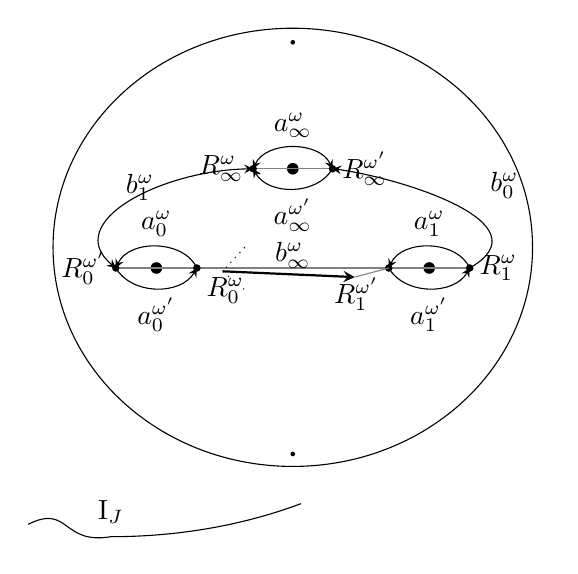
\begin{tikzpicture}[scale=1.05,>=stealth]
\draw[thin] (0,0) ellipse (2.9 and 2.65);
\fill (0,2.48) circle (.8pt);\fill (0,-2.5) circle (.8pt);
\fill (0,0.95) circle (2pt);\fill (-1.65,-0.25) circle (2pt);\fill (1.65,-0.25) circle (2pt);
\coordinate (ti) at (-.48,.95);\coordinate (tp) at (.48,.95);
\coordinate (li) at (-1.16,-.25);\coordinate (lp) at (-2.14,-.25);
\coordinate (ri) at (2.14,-.25);\coordinate (rp) at (1.16,-.25);
\draw[thin,gray] (ti)--(tp);\draw[thin,gray] (lp)--(ri);
\foreach \p in {ti,tp,li,lp,ri,rp}{\fill (\p) circle (1.3pt);}
\draw[<->] (ti) to[bend left=65] node[above] {$a_\infty^\omega$} (tp);
\draw[->] (tp) to[bend left=60] node[below] {$a_\infty^{\omega'}$} (ti);
\draw[->] (li) to[bend right=65] node[above] {$a_0^\omega$} (lp);
\draw[->] (lp) to[bend right=60] node[below] {$a_0^{\omega'}$} (li);
\draw[->] (ri) to[bend right=65] node[above] {$a_1^\omega$} (rp);
\draw[->] (rp) to[bend right=60] node[below] {$a_1^{\omega'}$} (ri);
\draw[<->] (ti) .. controls (-1.6,.93) and (-2.8,.30) .. (lp);
\node at (-1.85,.72) {$b_1^\omega$};
\draw[->] (ri) .. controls (3.1,.3) and (1.25,.85) .. (tp);
\node at (2.56,.75) {$b_0^\omega$};
\draw[dotted] (-.58,0)--(-.85,-.29)--(-.55,-.54);\draw[->,thick] (-.85,-.29)--(.75,-.36);
\draw[thin,gray] (.75,-.36)--(rp);\node at (0,-.10) {$b_\infty^\omega$};
\node[left] at (ti) {$R_\infty^\omega$};\node[right] at (tp) {$R_\infty^{\omega'}$};
\node[left] at (lp) {$R_0^{\omega'}$};\node[below right] at (li) {$R_0^\omega$};
\node[below left] at (rp) {$R_1^{\omega'}$};\node[right] at (ri) {$R_1^\omega$};
\node at (-2.2,-3.2) {$\mathrm I_J$};
\draw (-3.2,-3.35) .. controls (-2.7,-3.1) and (-2.8,-3.6) .. (-2.2,-3.5) .. controls (-1.1,-3.5) and (-.3,-3.25) .. (.1,-3.1);
\end{tikzpicture}}
$\unsure{\mathcal G_J|G_J}$ permute transitivement les six flèches $a_i^\omega$ et les six flèches $b_i^\omega$ : \deleted{\unsure{$R$}}
\[
(1)\quad\left\{\begin{aligned}
a_i^\omega &: R_i^\omega\mathbin{-}R_i^{\omega'}\\
b_i^\omega &: R_{\omega i}^\omega\longrightarrow R_{\omega'i}^{\omega'}
\end{aligned}\right.
\]
\[
(2)\quad\left\{\begin{aligned}
\mathrm a)\quad &b_i^\omega b_i^{\omega'}=1&&\text{(trois relations effectives)}\\
\mathrm b)\quad &a_i^\omega b_{\omega'i}^{\omega}a_i^{\omega'}b_{\omega i}^{\omega}
a_{\unsure{\omega'i|\omega i}}^{\omega'}b_i^\omega=1&&\text{(deux relations effectives, une pour chaque }\omega\in\uline{\omega}\text{)}
\end{aligned}\right.
\]
\margin{\uline{NB}\quad $\tau(R_i^\omega)=R_i^\omega$\quad $\tau(a_i^\omega)=(a_i^{\omega'})^{-1}$\quad $\tau(b_i^\omega)=b_i^\omega$.}
\[
(3)\quad a_i^{\omega'}a_i^\omega=\lambda_i^\omega=\varphi_i^\omega(l_0)
\]
\[
(4)\quad \varphi_i^\omega:\quad
\Pi_{03}=\Pi_1(\unsure{U_{0,3}|\mathbf U_{0,3}};R_0^+)=\{l_0,l_1,l_\infty\mid l_0l_1l_\infty=1\}
\subset\widetilde\Pi_{0,3}=\Pi_1(\unsure{U_{0,3}|\mathbf U_{0,3}},\unsure{\mathcal G_J|G_J} R_0^+\unsure{)}
\]
\diagram{\begin{tikzcd}[ampersand replacement=\&,column sep=large]
\Pi_{03}\arrow[r]\&\Pi_1(\Sigma^*,R_i^\omega)
\end{tikzcd}}
\[
\begin{aligned}
l_0&\longmapsto a_i^{\omega'}a_i^\omega\\
l_1&\longmapsto (\unsure{b_{\omega i}^\omega|b_\infty^\omega})^{-1}a_{\omega i}^{\omega}a_{\omega i}^{\omega'}b_i^\omega
\end{aligned}
\]
Les $\varphi_i^\omega$ sont \unsure{permutés} entre eux \unsure{par les|par des} \unsure{formules} simples \unsure{de} transition
\[
(5)\quad\tau\varphi_i^\omega(g)=\varphi_i^\omega(\tau_\infty(g))
\qquad\text{où}\quad\tau_\infty\in\widetilde\Pi_{0,3}
\qquad\left\{\begin{aligned}
\tau_\infty(l_0)&=l_0^{-1}\\
\tau_\infty(l_1)&=l_1^{-1}\\
\tau_\infty(l_\infty)&=l_0l_1=\operatorname{int}(l_0)l_\infty^{-1}
\end{aligned}\right.
\]
\[
(6)\quad\left\{\begin{aligned}
a_i^\omega(\varphi_i^\omega(g))&=\varphi_i^{\omega'}(\varepsilon_0(g))\\
b_i^\omega(\varphi_{\omega i}^\omega(g))&=\varphi_{\omega'i}^{\omega'}(\sigma_\infty(g))
\end{aligned}\right.
\qquad\varepsilon_0^2=l_0
\]
\[
\begin{aligned}
\sigma_\infty(l_0)\unsure{'}&=l_1\\
\sigma_\infty(l_1)&=l_0\\
\sigma_\infty(l_\infty)&=(l_0l_1)^{-1}=l_1^{-1}l_0^{-1}=\operatorname{int}(l_0)l_\infty
\end{aligned}
\]
\deleted{$\unsure{\widetilde b_{\omega'i}^\omega|\widetilde b_i^\omega}$}

On introduit
\[
(7)\quad\widetilde b_i^\omega=a_{\omega'i}^{\omega'}b_i^\omega:
R_{\omega i}^\omega\mathbin{-}R_{\omega'i}^\omega,
\]
donc (2b) s'écrit
\[
(8)\quad\widetilde b_{\omega^2i}^\omega\widetilde b_{\omega i}^\omega\widetilde b_i^\omega=1
\]
\margin{\uline{NB} L'ens des $\widetilde b_i^\omega$ n'est pas stable sous $\tau$ il faudrait donc \unsure{aussi} prendre les $\tau\widetilde b_i^\omega$}
On aura
\[
(9)\quad\widetilde b_i^\omega(\varphi_{\omega i}^\omega(g))=\varphi_{\omega'i}^\omega(\rho^{-1}(g))
\qquad\rho^{-1}=\varepsilon_0\sigma_\infty
\qquad\left\{\begin{aligned}
\rho(l_0)&=l_1\\
\rho(l_1)&=l_\infty\\
\rho(l_\infty)&=l_0
\end{aligned}\right.
\]
Les relations 2bis deviennent
\[
(\unsure{10})\quad\widetilde b_{\omega^2i}\widetilde b_{\omega i}\widetilde b_i=1
\]
\margin{23}

\scanpage{25}
\mspage{6}
\margin{\uuline{endomorphismes} serait plus exact --- on ne sait pas alors \unsure{exprimer}, en termes de $(p,\beta)$, que $u$ est un \uuline{automorphisme}. \unsure{Ça revient à un|Ça n'est pas un} endomorphisme, \unsure{imposant} seulement $p\in\widehat{\mathbb Z}$, non $p\in\widehat{\mathbb Z}^{*}$, en tous cas $p$ de la forme $2\gamma+1$, avec $\gamma\in\widehat{\mathbb Z}$.}
$u$ autom \inserted{du groupoïde $\widehat{\mathrm{II}}_J$} qui commute à $\unsure{\mathcal G_J|G_J}$, et fixe les pts,
\deleted{\unsure{fini et déterminé}}
et qui \unsure{invarie} \deleted{\unsure{tous}} les sous-groupoïdes $\widehat{\mathrm{II}}_{J,i}$, où $\widehat{\mathrm{II}}_{J,i}$ est engendré par $R_i^\omega$, $a_i^\omega$ \unsure{$\in$}, $\omega\in\uline{\omega}$. La condition : $\mathrm{II}_{J,i}$ \deleted{défini} donné par
\[
u(a_i^\omega)=a_i^\omega\underbrace{\varphi_{i\infty}^\omega(l_0^\gamma)}_{(\lambda_i^\omega)^\gamma}
=\varphi_i^{\omega'}(l_\infty^\gamma)a_i^\omega
\qquad\left|\begin{array}{l}l_0^\gamma\text{ indépendant de }i,\omega\\\gamma\in\widehat{\mathbb Z}\end{array}\right.
\]
on aura
\[
u(\deleted{\unsure{a}}a_i^{\omega'}a_i^\omega)=\varphi_{i\infty}(l_0^{2\gamma}\deleted{\unsure{1}}l_0)
\]
\[
u\bigl(\underbrace{\unsure{\varphi_{i\infty}^{\omega}|\varphi_{i\infty}^{\omega'}}(l_0)}_{\lambda_i^\omega}\bigr)
=\underbrace{\varphi_i^\omega(l_0^p)}_{(\lambda_i^\omega)^p}
\qquad\gamma=\frac{p-1}{2}
\]
\margin{faire les calculs en partant d'abord de $u(a_i^\omega)=a_i^\omega\varphi_i^\omega(\lambda)$ avec $\lambda\in\widehat\Pi_{0,3}$ qlc., (et non $\lambda$ de la forme $l_0^\gamma$, $\gamma\in\widehat{\mathbb Z}\ldots$)}
\[
\left\{\begin{aligned}
u(a_i^\omega)&=a_i^\omega\varphi_{i\infty}(l_0^\gamma)
&\gamma&=\frac{p-1}{2}\quad p\in\widehat{\mathbb Z}^{*}\text{ multiplicateur}\\
u(b_i^\omega)&=b_i^\omega\varphi_{\omega i}^\omega(\deleted{\unsure{\xi}}\beta)
&\beta&\in\widehat\Pi_{0,3}\\
&\deleted{\unsure{\varphi_{\omega'i}^{\omega'}(\beta)b_i^\omega}}\quad
\inserted{\bigl(=\varphi_{\omega'i}^{\omega'}(\tau_\infty\beta)b_i^\omega\bigr)}
\end{aligned}\right.
\]
Ici \deleted{\unsure{le}} $(p,\beta)$ détermine $u$ (en fait, $\beta$ détermine $p\ldots$)
\[
u(\widetilde b_{\unsure{t}i}^\omega)=\widetilde b_i^\omega\varphi_{\omega i}^\omega
\bigl(\underbrace{l_1^{-\gamma}\beta}_{\unsure{\sigma_\infty(\lambda)}\beta}\bigr)
=\varphi_{\omega'i}^{\omega'}\bigl(l_0^{-\gamma}\rho^{-1}(\beta)\bigr)\widetilde b_i^\omega
\]
Les équations sur $(p,\beta)$ équivalent à \unsure{sont|$\longrightarrow$}
\[
(12)\quad\left\{\begin{aligned}
\beta\sigma_\infty(\beta)&=1\\
\alpha\rho^{-1}(\alpha)\rho^{-2}(\alpha)&=1\\
\alpha&=\underbrace{l_1^{-\gamma}}_{\sigma_\infty(\lambda)}\beta
\end{aligned}\right.
\qquad\deleted{\text{où }\alpha=l_1^{-\gamma}\beta}\quad\text{ou}\quad
\bigl(\text{ou }\alpha^{-1}\rho(\alpha^{-1})\rho^2(\alpha^{-1})=1\bigr)
\]
\margin{\uline{NB} Si on remplace $\beta$ par $\beta^{-1}$, $\alpha$ par $\alpha^{-1}$ on retrouve les équations habituelles. cf plus bas}
\margin{Si on change la définition de $\beta$, en faisant que $\beta$ devienne $\sigma_\infty(\beta)$, les deux premières équations (12) restent pareilles mais $\alpha=l_1^{\unsure{\gamma}}\sigma_\infty(\beta)$, ce qui est un peu moins joli\ldots\ et est \unsure{évident} \unsure{que} $\beta\mapsto\beta'$.}
Notons que si $u$ est défini par \inserted{$(p,$}\deleted{$\beta$}\inserted{$\beta)$}, alors
$\tau(u)$ \inserted{$=\tau u\tau^{-1}$} est défini par $(p,\beta'=\tau_\infty(\beta))$. Il faudrait pouvoir vérifier directement, par un calcul dans $\Pi_{0,3}$, que les équations (12) en $\beta$, impliquent les $\Rightarrow$ relations pour $\beta'=\tau_\infty(\beta)$ (avec $\unsure{\gamma\prime|\gamma}=\gamma$).
\margin{24}

\scanpage{26}
\mspage{7}
\figure{
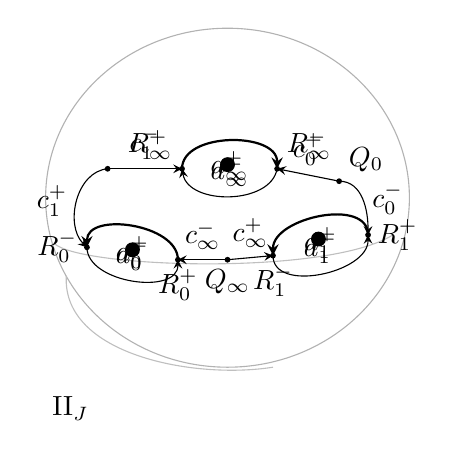
\begin{tikzpicture}[x=1.05cm,y=1.05cm,>=stealth]
\draw[gray!60] (0,.65) ellipse (2.2 and 2.05);
\draw[gray!50] (-2.1,.1) .. controls (-1.8,-.2) and (1.2,-.3) .. (2,.2);
\draw[gray!50] (-1.95,-.3) .. controls (-2,-1.25) and (-.4,-1.55) .. (.55,-1.4);
\coordinate (A) at (-.55,1);\coordinate (B) at (.6,1);
\coordinate (C) at (-1.7,.05);\coordinate (D) at (-.6,-.1);
\coordinate (E) at (.55,-.05);\coordinate (F) at (1.7,.2);
\coordinate (U) at (-1.45,1);\coordinate (V) at (1.35,.85);\coordinate (W) at (0,-.1);
\foreach \p in {A,B,C,D,E,F,U,V,W}{\fill (\p) circle (.035);}
\fill (0,1.05) circle (.09);\fill (-1.15,.02) circle (.09);\fill (1.1,.15) circle (.09);
\draw[->,thick] (A) to[out=90,in=90] node[below] {$a_\infty^+$} (B);
\draw[->] (B) to[out=260,in=280] node[above] {$a_\infty^-$} (A);
\draw[->,thick] (D) to[out=90,in=90] node[below] {$a_0^+$} (C);
\draw[->] (C) to[out=270,in=270] node[above] {$a_0^-$} (D);
\draw[->,thick] (F) to[out=90,in=90] node[below] {$a_1^+$} (E);
\draw[->] (E) to[out=270,in=270] node[above] {$a_1^-$} (F);
\draw[->] (U) to[out=185,in=135] node[left] {$c_1^+$} (C);
\draw[->] (U)--node[above] {$c_1^-$}(A);
\draw[->] (V)--node[above] {$c_0^+$}(B);
\draw[->] (V) to[out=0,in=90] node[right] {$c_0^-$}(F);
\draw[->] (W)--node[above] {$c_\infty^-$}(D);
\draw[->] (W)--node[above] {$c_\infty^+$}(E);
\node[above left] at(A){$R_\infty^+$};\node[above right] at(B){$R_\infty^-$};
\node[left] at(C){$R_0^-$};\node[below] at(D){$R_0^+$};
\node[below] at(E){$R_1^-$};\node[right] at(F){$R_1^+$};
\node[above right] at(V){$Q_0$};\node[below] at(W){$Q_\infty$};
\node at(-1.9,-1.9){$\mathrm{II}_J$};
\end{tikzpicture}
}
On rajoute les sommets $Q_i$ $(i\in J)$ et les arcs
\diagram{\begin{tikzcd}[ampersand replacement=\&]Q_i\arrow[r,"c_i^\omega"]\&R_{\omega'i}^{\omega'}\end{tikzcd}}
permutés \deleted{de façon \unsure{simplement} \unsure{transitivement}} par $G_J$. On a maintenant
\[
(13)\qquad b_i^\omega=c_i^\omega(c_i^{\omega'})^{-1}
\]
(donc les $b_i^\omega$ deviennent inutiles comme générateurs d'un groupoïde). \deleted{Les relations $(2)$ deviennent} \inserted{La} partie $(2)$ devient automatique, pour écrire commodément la partie $(3)$, introduit les
\[
(14)\qquad\widetilde a_i^\omega=
\deleted{(\unsure{c_{\omega i}^{\omega}})^{-1}a_i^{\unsure{\omega}}\unsure{c_{\omega'i}^{\omega'}}}
\inserted{(c_{\omega i}^\omega)^{-1}a_i^\omega c_{\omega'i}^{\omega'}}
:\quad Q_{\omega'i}\longrightarrow Q_{\omega i}
\]
\diagram{
\begin{tikzcd}[ampersand replacement=\&,column sep=small,row sep=large]
Q_{\omega i}\&R_i^{\omega'}\arrow[l,"(c_{\omega i}^{\omega})^{-1}"']\arrow[r,dashed,bend right=28,"a_i^{\omega'}"']\&R_i^\omega\arrow[l,bend right=45,"a_i^\omega"']\&Q_{\omega'i}\arrow[l,"c_{\omega'i}^{\omega'}"]\\
\deleted{\unsure{Q_{\omega i}}}\arrow[r,"\deleted{\unsure{c_{\omega i}^{\omega}}}"]\&\deleted{\unsure{R_i^\omega}}\arrow[r,bend right=45,"\deleted{a_i^{\omega'}}"']\&\deleted{\unsure{R_i^{\omega'}}}\arrow[r,"\deleted{(c_{\omega'i}^{\omega'})^{-1}}"']\&\deleted{\unsure{Q_{\omega'i}}}
\end{tikzcd}}
\margin{\figure{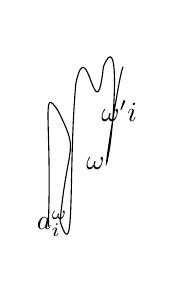
\begin{tikzpicture}[x=.5cm,y=.7cm]
\draw (0,0) .. controls (.1,1.9) and (-.2,2.6) .. (.25,2.1) .. controls (.8,1.3) and (.5,1.6) .. (.3,.1);
\draw (.3,.1) .. controls (.7,-.8) and (.5,1) .. (.7,2.6) .. controls (1,3.6) and (1.2,1.6) .. (1.4,2.9) .. controls (1.8,3.6) and (1.7,2.1) .. (1.55,1.4) .. controls (1.3,.4) and (1.8,2.8) .. (1.9,2.9);
\node at(.1,.05){$\unsure{a_i^\omega}$};\node at(1.2,1.15){$\unsure{\omega}$};\node at(1.8,2.1){$\unsure{\omega'i}$};
\end{tikzpicture}}}
qui sont également permutés de façon simpl. transitive sous $G_J$, et on a
\[
(15)\qquad\tau(\widetilde a_i^\omega)=(\widetilde a_i^{\omega'})^{-1}
\]
La relation $(2b)$ devient
\[
(16)\qquad\widetilde a_{\unsure{\omega\omega'i}}^\omega\widetilde a_{\omega i}^\omega\widetilde a_i^\omega=1
\]
(deux relations ess\textsuperscript{t.} distinctes qui sont permutées par $\tau$)

Pour repérer les \inserted{$\pi(Q_i)=$} $\pi_1(\Sigma_J(\mathbb C),Q_i)$ de façon commode on utilise les
\diagram{
\begin{tikzcd}[ampersand replacement=\&,column sep=large,row sep=large]
(17)\quad\psi_i^\omega:\ \deleted{\unsure{Q}}\Pi_{0,3}\arrow[rr,"\sim"]\arrow[dr,"\varphi_{\omega'i}^{\omega'}"',"\sim"]\&\&\pi(Q_i)\\
\&\pi(R_{\omega'i}^{\omega'})\arrow[ur,"(c_i^\omega)^{-1}"',"\sim"]\&
\end{tikzcd}}
\margin{\uline{NB}\quad$\tau\psi_i^\omega(g)=\psi_i^\omega(\tau_\infty g)$}
on aura
\[
(18)\qquad\psi_i^\omega(g)=\psi_i^{\omega'}(\sigma_\infty(g))
\]
\[
(19)\qquad\begin{aligned}
\widetilde a_i^{\unsure{\omega|\omega^*}}(\psi_{\omega'i}^{\omega'}(g))
&=\psi_{\unsure{\omega i}}^{\unsure{\omega}}(\varepsilon_0(g))
=\psi_{\unsure{\omega i}}^{\omega'}(\overbrace{\sigma_\infty\varepsilon_0}^{\deleted{\unsure{\xi}}\tau_\infty(\rho)}(g))\\
\boxed{\widetilde a_i^\omega(\psi_{\omega'i}^{\omega}(g))
=\psi_{\unsure{\omega i}}^{\unsure{\omega}}(\underbrace{\varepsilon_0\sigma_\infty}_{\rho^{-1}}(g))}
=\psi_{\omega i}^{\omega'}(\sigma_\infty\varepsilon_0\sigma_\infty(g))
\end{aligned}
\]
\margin{25}

\scanpage{27}
\mspage{8}
On prend un autom. $u$ du groupoïde $\widehat{\mathrm{II}}_J$ qui \inserted{commute à $G_J$ et qui} fixe les sommets, et qui comme plus haut laisse stables les sous-groupoïdes $\widehat{\mathrm{II}}_{J,i}$ $(i\in J)$, \deleted{\unsure{les groupoïdes}} $\mathrm{II}_{J,i}$ engendré par les \inserted{2} sommets $R_i^\omega$ $(\omega\in\uline{\omega})$ et les deux flèches $a_i^\omega$ $(\omega\in\uline{\omega})$.
\deleted{\unsure{Alors}} L'endom. $u$ est connu quand on connaît les $u(a_i^\omega)$, qui sont de la forme
\[
(20)\qquad u(a_i^\omega)=a_i^\omega\varphi_i^\omega\bigl(\underbrace{l_0^\gamma}_{\lambda}\bigr)
\qquad\begin{array}{l}\gamma=\frac{p-1}{2}\in\widehat{\mathbb Z}\\p\in\widehat{\mathbb Z}^{*}\end{array}
\]
\margin{NB: $\lambda\in\widehat\Pi_{0,3}$, pas la peine d'exiger de prime abord que $\lambda$ de la forme $l_0^\gamma\ldots$}
\uline{et} les
\[
(21)\qquad u(c_i^\omega)=\varphi_{\omega'i}^{\omega'}(\eta)c_i^\omega=c_i^\omega\psi_i^\omega(\eta)
\qquad\eta\in\widehat\Pi_{0,3}\quad\text{indépendant de }i,\omega
\]
On aura alors (comparer $(11)$)
\[
(22)\qquad u(b_i^\omega)=b_i^\omega\varphi_{\omega i}^\omega(\beta)\qquad\text{avec}
\]
\[
(23)\qquad\beta=\sigma_\infty(\eta)\eta^{-1}
\]
\margin{NB devient plus joli si $\eta$ est remplacé par son $\sigma_\infty\eta$, ou $\beta$ par $\beta^{-1}$}
Les relations à satisfaire sont alors déjà écrites en \inserted{$p$ (ou $\gamma$) et} $\beta$, \deleted{\unsure{la}} dans $(12)$ --- mais la première relation $\beta\sigma_\infty(\beta)=1$ conséquence de $(23)$, il reste la deuxième qui s'écrit donc
\margin{\uline{NB} Si $u$ remplacé par $u'=\tau(u)$, alors $\eta$ est remplacé par $\eta'=\tau_\infty(\eta)$, $\beta$ par $\tau_\infty(\beta)$, mais $\lambda$ par $\varepsilon_0^{-1}(\tau_\infty(\lambda^{-1}))$.}
\[
(24)\qquad\deleted{\unsure{(l_1^{-\gamma}\sigma_\infty(\eta)\eta^{-1}}}
\quad\alpha\rho^{-1}(\alpha)\rho^{-2}(\alpha)=1
\qquad\text{avec}\quad\alpha=\underbrace{l_1^{-\gamma}}_{\sigma_\infty(\lambda)}\underbrace{\sigma_\infty(\eta)\eta^{-1}}_\beta.
\]
On aura ici
\[
(25)\qquad
u(\widetilde a_i^\omega)=\psi_{\unsure{\omega i}}^{\unsure{\omega}}\bigl(\underbrace{\eta^{-1}l_0^\gamma\varepsilon_0(\eta)}_{\widetilde\alpha=\eta^{-1}\varepsilon_0(\lambda\eta)}\bigr)\widetilde a_i^\omega
=\widetilde a_i^\omega\psi_{\omega'i}^{\omega'}\bigl(\underbrace{\varepsilon_0^{-1}(\eta^{-1})l_0^\gamma\eta}_{\varepsilon_0^{-1}(\widetilde\alpha)}\bigr)
\]
\inserted{valable quel que soit $\lambda$}
\margin{$\widetilde\alpha=\eta^{-1}l_0^\gamma\varepsilon_0(\eta)$}
et
\[
(25\text{ bis})\quad\deleted{\unsure{\alpha=}}\quad\alpha=\rho\bigl(\eta\widetilde\alpha\rho^{-1}(\eta)^{-1}\bigr)
\]
\margin{valable pour $\lambda$ quelconque, pas \unsure{néc.} de la forme $l_0^\gamma$.}
\deleted{\unsure{car}} dans l'équation $(24)$ en $\alpha$ (invariante par substitutions $\alpha\mapsto\rho^{-1}(\alpha)$ (ou $\alpha\mapsto\rho\alpha=\rho^{-2}(\alpha)$) et $\alpha\mapsto x\alpha\rho^{-1}(x)^{-1}$,
\margin{26}

\scanpage{28}
\mspage{9}
équivaut à l'équation \deleted{\unsure{identique}} \deleted{\unsure{correspondante}} \inserted{\unsure{analogue}} en $\widetilde\alpha$
\[
(26)\qquad\widetilde\alpha\rho^{-1}(\widetilde\alpha)\rho^{-2}(\widetilde\alpha)=1,
\qquad\boxed{(27)\quad\widetilde\alpha=\eta^{-1}l_0^\gamma\varepsilon_0(\eta)}
\]
\deleted{$\unsure{\varepsilon}$}
Considérons maintenant le groupoïde \inserted{$\mathrm{III}_J$} induit par le groupoïde précédent \inserted{$\mathrm{II}_J$} sur l'ens des trois sommets $Q_i$, c'est aussi le groupoïde engendré par le graphe à trois sommets $Q_i$ $(i\in J)$ et six arcs orientés $\widetilde a_i^\omega$ et leurs opposés, avec les seules relations $(16)$ (ens de 6 relations stable par $G_J$, et se réduisant en fait à deux relations effectives\ldots).
\figure{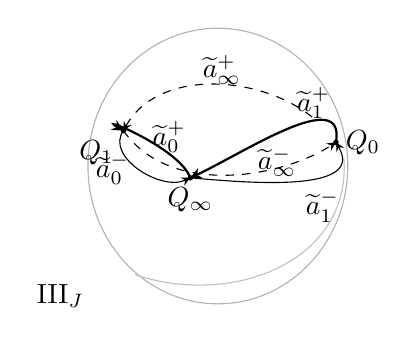
\begin{tikzpicture}[x=1cm,y=1cm,>=stealth]
\draw[gray!60] (0,.1) ellipse (1.65 and 1.75);
\draw[gray!50] (-1.05,-1.28) .. controls (.2,-1.7) and (1.7,-1.1) .. (1.6,.2);
\coordinate (A) at (-1.2,.55);\coordinate (B) at (-.35,-.05);\coordinate (C) at (1.5,.4);
\foreach \p in {A,B,C}{\fill(\p) circle(.035);}
\draw[->,thick] (B) to[out=110,in=150] node[right] {$\widetilde a_0^+$} (A);
\draw[->] (A) to[out=235,in=205] node[left] {$\widetilde a_0^-$} (B);
\draw[->,thick] (C) to[out=80,in=25] node[above right] {$\widetilde a_1^+$} (B);
\draw[->] (B) to[out=-5,in=300] node[below right] {$\widetilde a_1^-$} (C);
\draw[<-,dashed] (A) .. controls (-.75,1.35) and (.55,1.25) .. (1.2,.72);
\node at(.05,1.32){$\widetilde a_\infty^+$};
\draw[->,dashed] (A) .. controls (-.6,-.3) and (.8,-.05) .. (C);
\node at(.75,.15){$\widetilde a_\infty^-$};
\node[below left] at(A){$Q_1$};\node[below] at(B){$Q_\infty$};\node[right] at(C){$Q_0$};
\node at(-2,-1.55){$\mathrm{III}_J$};
\end{tikzpicture}}
Le groupe $\{1,\tau\}$ y opère dans le graphe avec relations, par
\[
(27)\qquad\tau Q_i=Q_i,\quad\tau\widetilde a_i^\omega=(\widetilde a_i^{\omega'})^{-1}
\]
La donnée d'un \deleted{\unsure{autom.}} \inserted{endom.} du groupoïde $\widehat{\mathrm{III}}_J$, fixant les sommets et commutant à $G_J$, équivaut alors à un $\widetilde\alpha\in\widehat\Pi_{0,3}$, \deleted{$\unsure{\in\widehat{\mathbb Z}}$}, satisfaisant \deleted{\unsure{l'équation rel.}} $(26)$. On aura, en introduisant
\[
(28)\qquad\widetilde\lambda_i^\omega=\widetilde a_i^{\omega'}\widetilde a_i^\omega\in\deleted{\unsure{Q_{\omega'i}}}\inserted{\pi(Q_{\omega'i})}
\]
(\unsure{comparer à la définition dans le groupoïde} $\mathrm{II}_J$ ! $\lambda_i^\omega=a_i^{\omega'}a_i^\omega$)
\diagram{\begin{tikzcd}[ampersand replacement=\&,column sep=small]
Q_{\omega i}\arrow[rrr,bend right=45,"\widetilde a_i^{\omega'}"']\&R_i^{\omega'}\arrow[l,dashed,no head]\arrow[r,dashed,bend right=40]\&R_i^\omega\arrow[l,dashed,bend right=40,"a_i^\omega"']\arrow[r,dashed,no head]\&Q_{\omega'i}\arrow[lll,bend right=45,"\widetilde a_i^{\unsure{\omega}}"']
\end{tikzcd}}
\margin{\deleted{il semblerait raisonnable de changer les notations $\widetilde a_i^\omega$ devenant $\widetilde a_i^{\omega'}$ \unsure{au-dessous}.}\quad $*$ \unsure{obtenir}, \unsure{une définition des} $\psi_i^\alpha$ \unsure{qui} \unsure{donne} dans $(29)$ \unsure{ainsi}. \unsure{cf.} \unsure{voir} plus bas}
\[
(29)\qquad u(\widetilde\lambda_i^\omega)=\overset{*}{\psi_{\omega'i}^{\omega'}}(\widetilde\alpha\varepsilon_0(\widetilde\alpha))\widetilde\lambda_i^\omega
=\psi_{\omega'i}^{\omega'}(\widetilde\alpha\varepsilon_0(\widetilde\alpha)l_0)
\]
Dans le cas où $\widetilde\alpha$ provient de $\eta,\gamma$ par $(27)$, on aura
\[
\widetilde\alpha\varepsilon_0(\widetilde\alpha)l_0=\eta^{-1}l_0^p\eta\qquad(p=2\gamma+1)\ ;
\]
\margin{27}

\scanpage{29}
\mspage{10}
\margin{\uline{NB} Ce sous-groupoïde $\mathrm{III}_{J,i}$ (de groupe fondamental $\widehat{\mathbb Z}$) engendré par les sommets $Q_j$ $(j\in J\setminus\{i\})$ et les deux $\unsure{\widetilde a_i^\omega}$ \unsure{orientés} qui les joignent, \uuline{n'est \deleted{\unsure{donc}} pas} stable \uline{par $u$} !}
\unsure{en|si} d'autres termes faisons opérer $u$ sur $\pi(Q_{\omega'i})$, identifié à $\widehat\Pi_{0,3}$ via $\psi_{\omega'i}^{\omega'}$, $\widetilde\lambda_i^\omega$ identifié à $l_0$, on trouve que $u(l_0)$ est conjugué de $l_0^p$, \deleted{avec} la conjugaison étant effectuée par $\eta^{-1}$ (par la formule $(30)$).

Le passage de $u$ à $\tau(u)$ s'exprime par
\deleted{J'en prends maintenant les points $P_\omega^{\unsure{\omega}}$ $(\omega\in\uline{\omega})$}
le passage de $\widetilde\alpha$ à
\[
(31)\qquad\widetilde\alpha'=\varepsilon_0\tau_\infty(\widetilde\alpha^{-1})
=\underbrace{\rho^{-1}\widetilde\sigma_\infty}_{\widetilde\sigma_0}(\widetilde\alpha^{-1})
\]
\margin{où $\widetilde\sigma_\infty=\sigma_\infty\tau_\infty=\tau_\infty\sigma_\infty$ est dans l'image de l'hom canonique
\diagram{\begin{tikzcd}[ampersand replacement=\&]\widetilde G_3\arrow[r]\&\widetilde\Pi_{0,3}\end{tikzcd}}
$\simeq$\quad\deleted{\unsure{du}\ $\widetilde G_3$}
stabilisateur de $P_+$ dans $G_3\times\{1,\tau\}$}
\[
\widetilde\sigma_i(l_i)=l_i^{-1}
\]
\[
\widetilde\sigma_i(l_j)=l_k^{-1}\quad\text{si }\{0,1,\infty\}=\{i,j,k\}
\]
\uline{NB} le groupe $\widetilde G_3$ opère sur $\Pi_{0,3}$ et contient \deleted{$\unsure{\xi}$} \deleted{\unsure{dont il}} $\{1,\rho^{-1},\rho^{-2}\}$ comme ss-groupe \inserted{$\widetilde G_3^+$} d'indice 2, \deleted{\unsure{dont $\widetilde G_3$ conjugue $\rho$}} $\widetilde G_3/\widetilde G_3^+$ opère sur $\widetilde G_3^+$ en échangeant $\rho$ et $\rho^{-1}$, il s'ensuit que $\widetilde G_3$ opère sur $V$ ens des solutions $x$ de l'équation
\[
x\rho^{-1}(x)\rho^{-2}(x)=1
\]
par
\[
(32)\qquad\Theta_g x=g.x^{\unsure{\operatorname{sg}(g)}}
\]
et on a ici
\[
(33)\qquad\widetilde\alpha'=\Theta_{\widetilde\sigma_0}(\widetilde\alpha)
\]
\margin{28}

\scanpage{30}
\margin{29}
\mspage{11}
\margin{\uline{NB} les flèches $\widetilde a_i^\omega$ sont en fait superflues, cf $(37)$ et commentaires p. 19.}
\figure{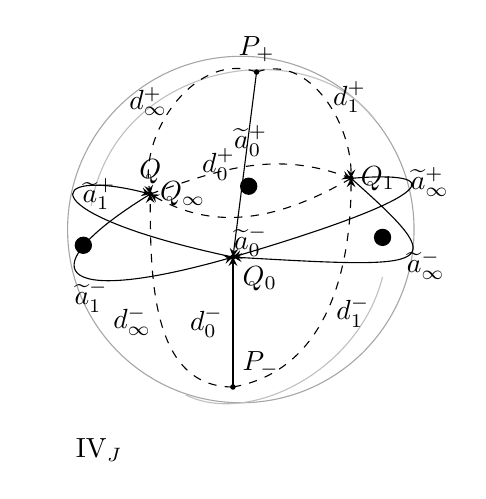
\begin{tikzpicture}[x=1cm,y=1cm,>=stealth]
\draw[gray!70] (0,0) ellipse (2.2 and 2.2);
\draw[gray!50] (-1.9,.3) .. controls (-1.6,2.1) and (.8,2.55) .. (1.7,1.4);
\draw[gray!50] (-.7,-2.1) .. controls (.1,-2.5) and (1.5,-1.8) .. (1.8,-.6);
\coordinate(P) at(.2,2);\coordinate(M) at(-.1,-2);\coordinate(A) at(-1.15,.45);\coordinate(B) at(1.4,.65);\coordinate(C) at(-.1,-.35);
\foreach \p in {P,M,A,B,C}{\fill (\p) circle(.035);}
\fill (-2,-.2) circle(.11);\fill(.1,.55) circle(.11);\fill(1.8,-.1) circle(.11);
\draw[->,dashed] (P) to[out=160,in=100] node[left]{$d_\infty^+$}(A);
\draw[->] (P)--node[left]{$d_0^+$}(C);
\draw[->,dashed] (P) to[out=20,in=90] node[right]{$d_1^+$}(B);
\draw[->,dashed] (M) to[out=180,in=270] node[left]{$d_\infty^-$}(A);
\draw[->] (M)--node[left]{$d_0^-$}(C);
\draw[->,dashed] (M) to[out=10,in=270] node[right]{$d_1^-$}(B);
\draw[->,dashed] (A) to[out=20,in=160] node[above]{$\widetilde a_0^+$}(B);
\draw[->,dashed] (B) to[out=210,in=330] node[below]{$\widetilde a_0^-$}(A);
\draw[->] (C) .. controls (-2.7,.2) and (-2.5,.8) .. (A);
\node at(-1.8,.45){$\widetilde a_1^+$};
\draw[->] (A) .. controls (-2.7,-.5) and (-2.4,-1) .. (C);
\node at(-1.9,-.85){$\widetilde a_1^-$};
\draw[->] (B) .. controls (2.6,.75) and (2.6,.45) .. (C);
\node at(2.4,.6){$\widetilde a_\infty^+$};
\draw[->] (B) .. controls (2.7,-.5) and (2.5,-.5) .. (C);
\node at(2.35,-.45){$\unsure{\widetilde a_\infty^-}$};
\node[above] at(P){$P_+$};\node[above right] at(M){$P_-$};
\node[right] at(A){$Q_\infty$};\node[right] at(B){$Q_1$};\node[below right] at(C){$Q_0$};
\node[above] at(A){$\deleted{\unsure{Q}}$};\node at(-1.8,-2.8){$\mathrm{IV}_J$};
\end{tikzpicture}}
On rajoute les \inserted{deux} sommets $\unsure{P_i^\omega|P_\infty^\omega}$ $(\omega\in\uline{\omega})$, et les flèches
\diagram{\begin{tikzcd}[ampersand replacement=\&]d_i^\omega:\quad P_\infty^\omega\arrow[r]\&Q_i\end{tikzcd}}
permutés transitivement par $G_J$, avec
\[
(34)\qquad\tau(P_{\unsure{\infty|i}}^\omega)=P_{\unsure{\infty|i}}^{\omega'},\qquad\tau(d_i^\omega)=d_i^{\omega'}
\]
Le groupoïde $\mathrm{III}_J$ est équivalent au groupoïde $\mathrm{IV}_J$ \inserted{défini par le graphe ayant} \deleted{sur} les sommets $Q_i$ $(i\in\unsure{\omega|J})$ et $P_\infty^\omega$ $(\omega\in\uline{\omega})$, les arcs $\widetilde a_i^\omega$ et $d_i^\omega$ et les \inserted{arcs} opposés, et les six relations
\[
(35)\qquad(d_{\omega'i}^\omega)^{-1}\widetilde a_{\omega i}^{\omega}d_i^\omega=1
\]
(qui impliquent d'ailleurs les relations constitutives $(16)$ pour $\mathrm{III}_J$). La donnée d'un endomorphisme de $\mathrm{IV}_J$ qui fixe les \deleted{pts} sommets (pour simplifier --- il faudra regarder aussi ceux qui permutent les sommets \inserted{$P_\omega$} en fixant les $Q_i$), \deleted{équivaut à} et qui commute à $G_J$, équivaut à la donnée des
\[
(36)\quad\left\{\begin{aligned}
u(\widetilde a_i^\omega)&=\psi_{\omega i}^\omega(\widetilde\alpha)\widetilde a_i^\omega
&\widetilde\alpha&\in\widehat\Pi_{0,3}\quad\text{(indép. de }i,\omega\text{)}\\
u(d_i^\omega)&=\psi_i^\omega(\xi)d_i^\omega\quad\bigl(=d_i^\omega\widetilde\psi_i^\omega(\xi)\bigr)
&\xi&\in\widehat\Pi_{0,3}\quad\cdots
\end{aligned}\right.
\]
\deleted{\unsure{u}}
de $\widetilde\alpha,\xi\in\widehat\Pi_{0,3}$, avec la relation déduite de $(35)$, on trouve les équations
\[
(37)\qquad\widetilde\alpha=\xi.\rho^{-1}(\xi^{-1}),
\]
i.e. $\widetilde\alpha$ est connu quand on connaît $\xi\in\widehat\Pi_{0,3}$.
\margin{il n'y a donc pas de condition sur $\xi$ ici.}

\scanpage{31}
\mspage{12}
qui implique bien sûr (26).

\margin{\unsure{revenant} \unsure{avant} l'introduction de $u$}
Je \deleted{vais} considère les isomorphismes
\diagram{\begin{tikzcd}[ampersand replacement=\&,column sep=large,row sep=large]
\Pi_{0,3}\arrow[r,"\widetilde\psi_i^\omega"]\arrow[dr,"\psi_i^\omega"']\&\pi(P^\omega)\\
\&\pi(Q_i)\arrow[u,"(d_{\unsure{i}}^\omega)^{-1}"']
\end{tikzcd}}\quad(38)
\margin{\uline{NB} le passage de $u$ à $\tau(u)$ s'exprime par
$\xi\mapsto\sigma_\infty\tau_\infty(\xi)=\widetilde\sigma_\infty(\xi)$}
\margin{\deleted{\unsure{Changement} \unsure{de base} de l'iso $\Pi_{0,3}\simeq\Pi_{0,3}$ pour \unsure{compatib.}}}

de sorte que les relations (35) et (19) donnent
\[
(39)\qquad \widetilde\psi_{\omega i}^\omega(g)=\widetilde\psi_i^\omega(\rho g)
\qquad\text{i.e.}\quad\widetilde\psi_{\omega i}=\widetilde\psi_i\circ\rho,
\]
\inserted{\figure{\begin{tikzpicture}\node[draw,ellipse] {$\rho^{-1}$?};\end{tikzpicture}}}
et j'introduis les chemins
\[
(40)\qquad\widetilde d_i^\omega:
\begin{tikzcd}[ampersand replacement=\&,column sep=large]
P_{\unsure{\infty|\xi}}^\omega\arrow[r,no head]\&P_{\unsure{\infty|\xi}}^{\omega'}
\end{tikzcd},\qquad
\widetilde d_i^\omega=(d_i^{\omega'})^{-1}d_i^\omega
\]
permutés de façon simplement transitive par $G_J$,
\deleted{\unsure{de} \unsure{\illegible{1}} et satisfaisant} satisfaisant
\[
(41)\qquad\tau(\widetilde d_i^\omega)=\widetilde d_i^{\omega'},\qquad
 d_i^\omega d_i^{\omega'}=1
\]
On \deleted{\unsure{aura donc}} les relations
\[
(42)\qquad\widetilde d_i^\omega(\widetilde\psi_i^\omega(g))=
\widetilde\psi_i^{\omega'}(\sigma_\infty(g)).
\]
Revenant à l'\deleted{auto}morphisme $u$, on aura \deleted{automatiquement}
\[
(43)\qquad u(\widetilde d_i^\omega)=\widetilde\psi_i^{\omega'}(\unsure{\sigma_\infty}(\widetilde\beta))\widetilde d_i^\omega
=\widetilde d_i^\omega\widetilde\psi_i^\omega(\widetilde\beta)
\]
avec
\[
(44)\qquad\widetilde\beta=\xi\sigma_\infty(\xi)^{-1}.
\]
satisfaisant \inserted{donc} \deleted{\unsure{ainsi}} comme $\widetilde\beta$ doit, la relation
\[
(45)\qquad\widetilde\beta\sigma_\infty(\widetilde\beta)=1.
\]

Considérons maintenant les ss-groupes de
\margin{30}

\scanpage{32}
\mspage{13}
\figure{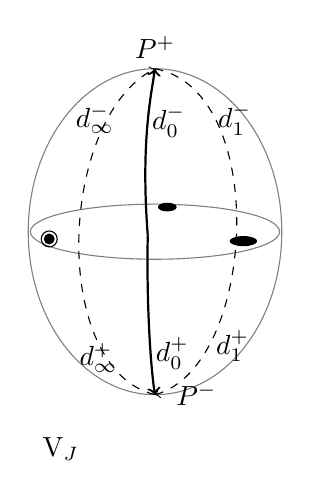
\begin{tikzpicture}[scale=.92]
\draw[gray] (0,0) ellipse (1.75 and 2.25);
\draw[gray] (0,0) ellipse (1.72 and .38);
\fill (-1.46,-.10) circle (.075);\draw (-1.46,-.10) circle (.11);
\fill (.17,.34) ellipse (.13 and .06);
\fill (1.22,-.13) ellipse (.19 and .07);
\draw[->,thick] (-.1,-.05).. controls (-.2,1.25) and (-.05,1.9)..(0,2.25);
\draw[->,thick] (-.1,-.05).. controls (-.12,-1.1) and (-.05,-1.95)..(0,-2.25);
\draw[dashed,->] (0,-2.25)..controls (-1.45,-1.9) and (-1.35,1.55)..(0,2.25);
\draw[dashed,->] (0,2.25)..controls (1.6,1.95) and (1.4,-1.85)..(0,-2.25);
\node[above] at (0,2.25) {$P^+$};\node[right] at (.16,-2.25) {$P^-$};
\node at (-.83,1.55) {$d_\infty^-$};\node at (.19,1.52) {$d_0^-$};\node at (1.1,1.55) {$d_1^-$};
\node at (-.78,-1.74) {$d_\infty^+$};\node at (.24,-1.68) {$d_0^+$};\node at (1.07,-1.58) {$d_1^+$};
\node at (-1.3,-3) {$\mathrm{V}_J$};
\end{tikzpicture}}
$\mathrm{IV}_J$, \deleted{formé des} \inserted{induit sur les} deux sommets $P^\omega$ \deleted{et $P^-$} $(\omega\in\uline{\omega})$, on peut le regarder comme le groupoïde libre engendré par le graphe de $=$ nom $\mathrm{V}_J$, ayant ces deux sommets, et trois arêtes --- donnant lieu aux six arcs $d_i^\omega$ avec $d_i^{\omega'}$ et $d_i^\omega$ opposés --- arcs permutés \deleted{\unsure{transitive}} \inserted{de façon} \deleted{\unsure{ment}} \inserted{\unsure{simplet.}} par \deleted{les} $G_J$. Un \deleted{autom.} \inserted{endom.} de ce groupoïde qui fixe les sommets est déterminé par les
\[
(46)\qquad u(\widetilde d_i^\omega)=\widetilde d_i^\omega\widetilde\psi_i^\omega(\widetilde\beta)
\qquad\text{avec }\widetilde\beta\in\widehat\Pi_{0,3}\quad\text{indépendant de }i,\omega
\]
La seule relation à satisfaire correspond aux équations $d_i^{\omega'}d_i^\omega=1$, qui donne
\[
(47)\qquad\widetilde\beta\sigma_\infty(\widetilde\beta)=1
\]
\figure{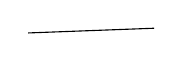
\begin{tikzpicture}\draw (0,0)--(1.6,.06);\end{tikzpicture}}

Considérons enfin le groupoïde induit sur les \deleted{pts} sommets $R_i^\omega,Q_i,P^\omega$ $(6+3+2=11\text{ sommets})$,
\margin{31}

\scanpage{33}
\mspage{14}
\figure{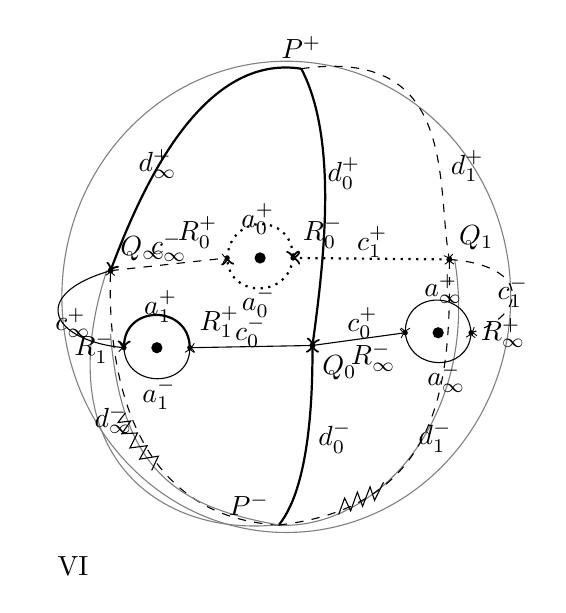
\begin{tikzpicture}[scale=.95]
\draw[gray] (0,0) ellipse (3 and 3.15);
\draw[gray] (-2.4,.35)..controls (-3.2,-2.1) and (-1.7,-3.2)..(-.15,-3.05);
\draw[gray] (2.25,.5)..controls (2.6,-1.6) and (1.2,-3.15)..(-.15,-3.05);
\coordinate (Pp) at (.2,3.05);\coordinate (Pm) at (-.1,-3.05);
\coordinate (Qi) at (-2.35,.35);\coordinate (Qz) at (.35,-.65);\coordinate (Qo) at (2.18,.5);
\draw[->,thick] (Pp)..controls (-1.1,3.25) and (-1.9,1.55)..(Qi);
\draw[->,thick] (Pp)..controls (.7,2.1) and (.5,.45)..(Qz);
\draw[dashed,->] (Pp)..controls (2.3,3.35) and (2,1.5)..(Qo);
\draw[dashed,->] (Pm)..controls (-1.95,-2.95) and (-2.4,-1.2)..(Qi);
\draw[->,thick] (Pm)..controls (.35,-2.5) and (.35,-1.1)..(Qz);
\draw[dashed,->] (Pm)..controls (2.1,-2.8) and (2.2,-1.1)..(Qo);
\draw[gray] (-2.35,-.5)..controls (-2.2,-2.3) and (-1.5,-2.8)..(-.1,-3.05);
\draw (-2.15,-1.55)--(-2.25,-1.68)--(-2.08,-1.66)--(-2.2,-1.83)--(-1.99,-1.82)--(-2.09,-2.02)--(-1.86,-1.99)--(-1.96,-2.17)--(-1.71,-2.13)--(-1.8,-2.32);
\draw (.7,-2.91)--(.78,-2.69)--(.86,-2.86)--(.95,-2.61)--(1.02,-2.8)--(1.12,-2.54)--(1.18,-2.72)--(1.3,-2.48);
\foreach \p in {Qi,Qz,Qo}{\fill (\p) circle (.04);}
\node[above] at (Pp) {$P^+$};\node[above left] at (Pm) {$P^-$};
\node[above right] at (Qi) {$Q_\infty$};\node[below right] at (Qz) {$Q_0$};\node[above right] at (Qo) {$Q_1$};
\node at (-1.72,1.78) {$d_\infty^+$};\node at (.77,1.65) {$d_0^+$};\node at (2.42,1.75) {$d_1^+$};
\node at (-2.31,-1.64) {$d_\infty^-$};\node at (.65,-1.88) {$d_0^-$};\node at (1.99,-1.87) {$d_1^-$};
\fill (-.35,.52) circle (.075);\fill (-1.73,-.68) circle (.075);\fill (2.03,-.48) circle (.075);
\coordinate (Rzp) at (-.79,.52);\coordinate (Rzm) at (.09,.52);
\coordinate (Rom) at (-2.17,-.68);\coordinate (Rop) at (-1.29,-.68);
\coordinate (Rim) at (1.59,-.48);\coordinate (Rip) at (2.47,-.48);
\draw[dotted,thick,->] (Rzp)..controls (-.75,1.12) and (.07,1.12)..(Rzm);
\draw[dotted,thick,->] (Rzm)..controls (.03,-.02) and (-.75,-.02)..(Rzp);
\draw[->,thick] (Rop)..controls (-1.3,-.1) and (-2.16,-.1)..(Rom);
\draw[->] (Rom)..controls (-2.15,-1.23) and (-1.3,-1.23)..(Rop);
\draw[->] (Rip)..controls (2.43,.1) and (1.6,.1)..(Rim);
\draw[->] (Rim)..controls (1.65,-1.01) and (2.43,-1.01)..(Rip);
\foreach \p in {Rzp,Rzm,Rom,Rop,Rim,Rip}{\fill (\p) circle (.035);}
\node[above left] at (Rzp) {$R_0^+$};\node[above right] at (Rzm) {$R_0^-$};
\node[left] at (Rom) {$R_1^-$};\node[above right] at (Rop) {$R_1^+$};
\node[below left] at (Rim) {$R_\infty^-$};\node[right] at (Rip) {$R_\infty^+$};
\node at (-.38,1.04) {$a_0^+$};\node at (-.37,-.07) {$a_0^-$};
\node at (-1.68,-.13) {$a_1^+$};\node at (-1.7,-1.3) {$a_1^-$};
\node at (2.1,.11) {$a_\infty^+$};\node at (2.14,-1.08) {$a_\infty^-$};
\draw[dashed,->] (Qi)--(Rzp);\node at (-1.57,.67) {$c_\infty^-$};
\draw[->] (Qi)..controls (-3.45,.03) and (-3.15,-.58)..(Rom);\node at (-2.85,-.35) {$c_\infty^+$};
\draw[dotted,thick,->] (Qo)--(Rzm);\node at (1.15,.73) {$c_1^+$};
\draw[dashed,->] (Qo)..controls (3.3,.42) and (3.2,-.26)..(Rip);\node at (3.03,.07) {$c_1^-$};
\draw[->] (Qz)--(Rop);\node at (-.48,-.47) {$c_0^-$};
\draw[->] (Qz)--(Rim);\node at (1.02,-.35) {$c_0^+$};
\node at (-2.85,-3.6) {$\mathrm{VI}$};
\end{tikzpicture}}
C'est le groupoïde engendré par ces sommets, les arêtes $a_i^\omega,c_i^\omega,d_i^\omega$ (trois paquets, \deleted{\unsure{permutés}} \inserted{ch. un} un torseur sous $G_J$) et les \inserted{\unsure{six}} relations
\[
(48)\qquad(d_{\omega i}^\omega)^{-1}(c_{\omega i}^{\omega'})^{-1}(a_{\omega i}^\omega)^{-1}c_i^\omega d_i^\omega=1
\]
\deleted{\unsure{Hom.}} L'automorphisme $\tau$ est donné par
\[
(49)\qquad\left\{\begin{aligned}
\tau(R_i^\omega)&=R_i^{\unsure{\omega|\omega'}},&\tau Q_i&=Q_i,&\tau(P_{\deleted{\unsure{\infty}}}^\omega)&=P^{\omega'}\\
\tau(a_i^\omega)&=(a_i^{\omega'})^{-1},&\tau(c_i^\omega)&=c_i^{\unsure{\omega'|\omega}},&\tau(d_i^\omega)&=d_i^{\omega'}
\end{aligned}\right.
\]
Les $\pi_1\unsure{\varepsilon}$ de les sommets $R_i^\omega,Q_i,P^\omega$ sont repérés respectivement, en termes de $\Pi_{0,3}$, par les isomorphismes
\[
(50)\qquad\left\{\begin{gathered}
\begin{tikzcd}[ampersand replacement=\&,column sep=large]
\Pi_{0,3}\arrow[r,"\varphi_i^\omega"]\&\pi(R_i^\omega)\deleted{\longrightarrow\pi(}
\end{tikzcd}\\
\begin{tikzcd}[ampersand replacement=\&,column sep=large]
\Pi_{0,3}\arrow[r,"\psi_i^\omega"]\&\pi(Q_i)
\end{tikzcd}\\
\begin{tikzcd}[ampersand replacement=\&,column sep=large]
\Pi_{0,3}\arrow[r,"\widetilde\psi_i^\omega"]\&\pi(P^\omega)
\end{tikzcd}
\end{gathered}\right.
\]
reliés entre eux par les relations suivantes, qui \deleted{les} expriment \deleted{les} \inserted{les $\psi_i^\omega,\widetilde\psi_i^\omega$} en termes des $\varphi_i^\omega$
\[
(51)\qquad\deleted{\unsure{\widetilde d_i^\omega}}\left\{\begin{aligned}
d_i^\omega(\widetilde\psi_i^\omega(g))&=\psi_i^\omega(g)\\
\deleted{\unsure{\psi_i^\omega}}c_i^\omega\psi_i^\omega(g)&=\varphi_i^\omega(g)
\end{aligned}\right.
\]
On a, pour mémoire
\[
(52)\qquad\psi_i^\omega(g)=\psi_i^{\omega'}(\sigma_\infty(g))
\]
\margin{32}

\scanpage{34}
\mspage{15}
\[
(53)\qquad a_i^\omega\varphi_i^\omega(g)=\varphi_i^{\omega'}(\varepsilon_0(g))
\]
La donnée d'un endomorphisme du groupoïde \inserted{profini}, fixant les sommets et qui commute à $G_J$, équivaut à celle des \deleted{éléments} transformés des $a_i^\omega,c_i^\omega,d_i^\omega$, de façon \deleted{qui} compatible à l'action \unsure{de|des} $G_J$, et de façon à satisfaire aux relations (48).

On aura
\[
(54)\qquad\left\{\begin{aligned}
u(a_i^\omega)&=a_i^\omega\varphi_i^\omega(\lambda)\\
u(c_i^\omega)&=\varphi_{\omega'i}^{\omega'}(\eta)c_i^\omega=c_i^\omega\psi_{\unsure{0|i}}^\omega(\eta)\\
u(d_i^\omega)&=\psi_i^\omega(\xi)d_i^\omega=d_i^\omega\widetilde\psi_i^\omega(\xi)
\end{aligned}\right.
\]
avec $\lambda,\xi,\eta\in\widehat\Pi_{0,3}$, soumis à la seule relation déduite de (48). Au lieu de refaire le calcul, un peu fastidieux, pour expliciter la relation en $(\lambda,\eta,\xi)$, je préfère noter que le \deleted{le} groupoïde envisagé est la réunion des groupoïdes $\mathrm{II}$ et $\mathrm{IV}$, dont l'intersection est $\mathrm{III}$, donc \inserted{la donnée d'}un endom. \inserted{(fixant les sommets et comm. à $G_J$)} revient à celle d'un \inserted{tel} endom. $(\lambda,\eta)$ de $\mathrm{II}$, et d'un autre tel endom. \inserted{$\xi$} de $\mathrm{IV}$, de telle façon qu'ils se recollent \deleted{\unsure{en} \unsure{dans} $\mathrm{III}$} par un $=$ endomorphisme $(\widetilde\alpha)$ de $\mathrm{III}$, i.e tels qu'on ait à la fois
\[
(55)\qquad\widetilde\alpha=\eta^{-1}\varepsilon_0(\lambda\eta)\qquad\text{et}\qquad
\widetilde\alpha=\xi\rho^{-1}(\xi^{-1})
\]
\margin{33}

\scanpage{35}
\mspage{16}
L'équation à satisfaire par $(\lambda,\eta)$ se réduit, on a vu, à $\unsure{\rho|\{}\ \widetilde\alpha\rho^{-1}(\widetilde\alpha)\rho^{-2}(\widetilde\alpha)$, avec $\widetilde\alpha$ donné en fonction de $(\lambda,\eta)$ par la première \deleted{relation} \inserted{formule} (55) --- mais cette relation \inserted{en $\widetilde\alpha$} est conséquence de la seconde relation (55), donnant $\widetilde\alpha$ en termes de $\xi$. Il reste donc, comme relation reliant $\lambda,\eta,\xi$, que la relation (55) sous la forme (où ne figure plus $\unsure{\widehat\alpha|\widetilde\alpha}$)
\[
(56)\qquad\eta^{-1}\varepsilon_0(\lambda\eta)=\xi\rho^{-1}(\xi)^{-1}
\]
Je vais la mettre sous une forme plus familière pour moi, en introduisant d'abord les quantités précédentes
\[
(57)\qquad\left\{\begin{aligned}
\beta&=\sigma_\infty(\eta)\eta^{-1}
&&\bigl(u(b_i^\omega)=b_i^\omega\varphi_{\unsure{i\omega|\omega i}}^\omega(\beta)\bigr)\\
\alpha&=\sigma_\infty(\lambda)\beta
&&\bigl(u(\widetilde b_i^\omega)=\widetilde b_i^\omega\varphi_{\omega i}^\omega(\alpha)\bigr)\\
\widetilde\alpha&=\eta^{-1}\varepsilon_0(\lambda\eta)=\xi\rho^{-1}(\xi)^{-1}
&&\bigl(u(\widetilde a_i^\omega)=\psi_{\omega i}^\omega(\widetilde\alpha)\widetilde a_i^\omega\bigr)
\end{aligned}\right.
\]
et en les modifiant ainsi, ainsi que $\xi$:
\[
(58)\qquad\left\{\begin{aligned}
\beta'&=\beta^{-1}\inserted{=\sigma_\infty(\beta)}=\eta\sigma_\infty(\eta)^{-1}\\
\alpha'&=\alpha^{-1}=\beta^{-1}\sigma_\infty(\lambda)^{-1}=\beta'\sigma_\infty^{-1}(\lambda^{-1})\\
\deleted{\xi'}&\deleted{=\unsure{\eta}\,\unsure{\eta|\eta^{-1}}\xi}
\end{aligned}\right.
\]
\margin{donc $\beta'=\alpha'\sigma_\infty(\lambda)$}
\deleted{Je vais \unsure{ainsi|aussi} \unsure{considérer}, en introduisant \unsure{un mot} $\unsure{\gamma}$ \unsure{en} $\eta$.}
\deleted{\unsure{(59)}}
\deleted{Je dis que la relation (56) équivaut à}
\deleted{\unsure{(59)}}
En résumé, \unsure{$u$ est décrit} par les quantités \figure{\begin{tikzpicture}\node[draw,ellipse] {$\lambda,\eta,\xi'$};\end{tikzpicture}} $\in\widehat\Pi_{0,3}^{\unsure{3}}$ (équivalt à la donnée de $\lambda,\eta,\xi$), auxquelles j'associe $\alpha',\beta'$ par
\[
(59)\qquad\begin{aligned}
\beta'&=\eta\sigma_\infty(\eta)^{-1}\deleted{\unsure{\sigma_0(\lambda\eta)}}\\
\deleted{\unsure{d'}}\alpha'&=\deleted{\unsure{\beta}}\beta'\sigma_\infty(\lambda^{-1})
\qquad\text{i.e.}\quad\beta'=\alpha'\sigma_\infty(\lambda)
\end{aligned}
\]
\margin{34}

\scanpage{36}
\mspage{17}
et ceci posé, la relation (56) équivaut à
\[
(60)\qquad\left\{\begin{aligned}
\alpha'&=\xi'\unsure{\rho|\rho^{-1}}(\xi')^{-1}\\
\text{i.e.}\quad\eta\sigma_\infty(\eta)^{-1}&=(\xi'\rho(\xi')^{-1})\sigma_\infty(\lambda)
\end{aligned}\right.
\]
\deleted{i.e. à}\quad\deleted{\unsure{(61)}}
En effet, la formule (25bis) exprimant $\alpha$ en termes de $\widetilde\alpha$
\[
(\unsure{x})\qquad\alpha=\rho(\eta\widetilde\alpha\rho^{-1}(\eta)^{-1})
\]
se récrit, en passant aux inverses et posant
\[
(\unsure{xx})\qquad\widetilde\alpha'=\widetilde\alpha^{-1}
\]
sous la forme
\[
(61)\qquad\alpha'=\rho(\rho^{-1}(\eta)\widetilde\alpha'\eta^{-1})
=\uline{\eta\rho(\widetilde\alpha')\rho(\eta)^{-1}}
\]
\deleted{et la formule}
(On considère ici $\alpha,\alpha',\widetilde\alpha,\widetilde\alpha'$ comme \unsure{déduits} de $\lambda,\eta\in\widehat\Pi_{0,3}$ par la première relation (55) pour ce qui est de $\widetilde\alpha$, dont les autres se déduisent par $(\unsure{x}),(\unsure{xx})$. D'ailleurs, la \inserted{2\textsuperscript{e}} formule (55) \deleted{\unsure{se}} s'écrit alors, en passant aux inverses
\[
\widetilde\alpha'=\rho^{-1}(\xi)\xi^{-1}
\]
i.e.
\[
\rho(\widetilde\alpha')=\xi\rho(\xi)^{-1}
\]
\deleted{de sorte que (61), \unsure{(62)} s'écrit encore}
\inserted{qui est équivalent \unsure{à (60)}}
\[
\alpha'=\eta\xi\rho(\xi^{-1}\eta^{-1})
\]
\deleted{i.e. \unsure{donc} à (60)},
i.e. à (60), avec
\[
\xi'=\eta\xi.
\]

\uline{En résumé} Les autom. du groupoïde $\mathrm{VI}_J$, induisant l'identité sur les sommets et \uline{commutant à l'action de $G_J$}, correspondent aux
\[
(62)\qquad\boxed{(\lambda,\eta,\xi')\in\widehat\Pi_{0,3}\times\widehat\Pi_{0,3}\times\widehat\Pi_{0,3}}
\]
satisfaisant la relation des lacets \unsure{?|:}
\margin{35}

\scanpage{37}
\mspage{18}
\margin{Le passage de $u$ à $\tau(u)$ \unsure{s'effectue} par
\[
\begin{aligned}
\lambda&\longmapsto\varepsilon_0^{-1}(\tau_\infty(\lambda^{-1}))\\
(\lambda&\longmapsto\lambda\quad\text{si }\lambda=l_0^\gamma)\\
\eta&\longmapsto\tau_\infty(\eta)\\
\xi&\longmapsto\widetilde\sigma_\infty(\xi)=\sigma_\infty\tau_\infty(\xi)
\end{aligned}
\]}
\[
(63)\qquad\boxed{\boxed{\left\{\begin{aligned}
\beta'&=\alpha'\sigma_\infty(\lambda)\quad(=\alpha'l_1^\gamma\text{ si }\lambda=l_0^\gamma)\\
\text{avec}\qquad\alpha'&=\xi'\unsure{\rho|\rho^{-1}}(\xi')^{-1}\\
\beta'&=\eta\sigma_\infty(\eta)^{-1}
\end{aligned}\right.}}
\]
\margin{\uline{NB} L'\unsure{ens.} des relations stable par substitutions de la forme
\[
\begin{aligned}
\xi'&\longmapsto l_0^{\unsure{H|\mu}}\unsure{\xi|\xi\prime}\\
\eta&\longmapsto l_0^{\unsure{H|\mu}}\eta\\
\text{i.e.}\quad\alpha'&\longmapsto l_0^{\unsure{H|\mu}}\alpha'l_1^{-\unsure{H|\mu}}\\
\beta'&\longmapsto l_0^{\unsure{H|\mu}}\beta'l_1^{-\unsure{H|\mu}}
\end{aligned}
\]}
Ici, les quantités $\alpha',\beta',\xi'$ ont été introduites en termes des quantités primitives $\lambda,\eta,\xi$ $(\longmapsto\beta,\deleted{\unsure{\alpha}}\alpha,\widetilde\alpha)$, s'introduisant ds les formules (54) (et (57)), par le pur calcul \deleted{en} \inserted{dans} $\widehat\Pi_{0,3}$, comme donnant lieu aux formules les plus symétriques. Mais on peut les interpréter aussi de façon ``géométrique'', en posant (\deleted{\unsure{avant}} pour ce qui est de $\beta',\alpha',\widetilde\alpha'$)
\[
(64)\qquad\begin{aligned}
b_i^{\prime\omega}&=(b_i^\omega)^{-1}=b_i^{\omega'},\qquad
\unsure{(}\widetilde b_i^{\prime\omega}=(\widetilde b_i^\omega)^{-1},\qquad
\widetilde a_i^{\prime\omega}=(\widetilde a_i^\omega)^{-1}
\end{aligned}
\]
de sorte que les formules (57) deviennent
\[
(65)\qquad\left\{\begin{aligned}
u(b_i^{\prime\omega})&=\varphi_{\omega i}^\omega(\beta')b_i^{\prime\omega}\\
u(\widetilde b_i^{\prime\omega})&=\varphi_{\omega i}^\omega(\alpha')\widetilde b_i^{\prime\omega}\\
u(\widetilde a_i^{\prime\omega})&=\widetilde a_i^{\prime\omega}\psi_{\omega i}^\omega(\widetilde\alpha')
\end{aligned}\right.
\]
Enfin, la quantité $\xi'=\eta\xi$ est obtenue géométriquement, en introduisant les chemins
\diagram{\begin{tikzcd}[ampersand replacement=\&,column sep=large,row sep=large]
P^\omega\arrow[rr,"\widetilde d_i^{\prime\omega}"]\arrow[dr,"d_{\omega i}^\omega"']\&\&R_i^{\omega'}\\
\&Q_{\omega i}\arrow[ur,"c_{\omega i}^\omega"']\&
\end{tikzcd}}\quad(66)
\[
\widetilde d_i^{\prime\omega}=c_{\omega i}^\omega\cdot d_{\omega i}^\omega
\]
\figure{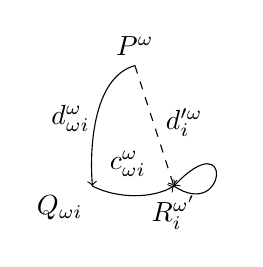
\begin{tikzpicture}[scale=.9]
\coordinate (P) at (.6,1.7);\coordinate (Q) at (0,0);\coordinate (R) at (1.15,0);
\draw[->] (P)..controls (.05,1.55) and (-.05,.65)..(Q);
\draw[dashed,->] (P)--(R);\draw[->] (Q)..controls (.35,-.18) and (.85,-.18)..(R);
\draw[->] (R)..controls (1.9,-.5) and (2,.9)..(R);
\node[above] at (P) {$P^\omega$};\node[below left] at (Q) {$Q_{\omega i}$};\node[below] at (R) {$R_i^{\omega'}$};
\node[left] at (.1,.95) {$d_{\omega i}^\omega$};\node[right] at (.9,.9) {$d_i^{\prime\omega}$};\node[above] at (.5,0) {$c_{\omega i}^\omega$};
\end{tikzpicture}}
par la formule
\margin{36}

\scanpage{38}
\mspage{19}
\[
(67)\qquad u(\widetilde d_i^{\prime\omega})=\varphi_i^{\omega'}(\underbrace{\xi'}_{\eta\xi})\widetilde d_i^{\prime\omega}
\]
On a aussi des chemins
\diagram{\begin{tikzcd}[ampersand replacement=\&,column sep=large,row sep=large]
P^\omega\arrow[rr,"d_i^\omega"]\arrow[dr,"d_{\omega'i}^\omega"']\&\&R_i^\omega\\
\&Q_{\omega'i}\arrow[ur,"c_{\omega'i}^{\omega'}"']\&
\end{tikzcd}}\quad(66')
\[
d_i^\omega=c_{\omega'i}^{\omega'}\cdot d_{\omega'i}^\omega
\]
\margin{\diagram{\begin{tikzcd}[ampersand replacement=\&,column sep=small,row sep=large]
\&P_\infty^\omega\arrow[d,"d_{\omega'i}^\omega"]\arrow[dl,dashed]\\
R_i^\omega\&Q_{\omega'i}\arrow[l,bend left=15,"c_{\omega'i}^{\omega'}"]
\end{tikzcd}}}
\margin{NB $\tau(d_i^\omega)=d_i^{\prime\omega}$}
et on aura également
\[
(67')\qquad u(\widetilde d_i^\omega)=\varphi_i^\omega(\eta\widetilde\sigma_\infty(\xi))\widetilde d_i^\omega
\]
\figure{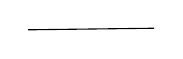
\begin{tikzpicture}\draw (0,0)--(1.6,.02);\end{tikzpicture}}

Je vois encore deux cas à regarder, savoir les sous-groupoïdes pleins de $\mathrm{VI}$ induits sur les \inserted{huit} sommets $(R_{i,\omega},P^\omega)$, soit $\mathrm{VII}$, décrit par le graphe de $=$ nom et les flèches $d_i^{\prime\omega},d_i^\omega,a_i^\omega,b_i^\omega$ (24 flèches), et celui induit sur les \deleted{cinq points} \inserted{sommets} $Q_i,P^\omega$ --- à strictement parler, c'est le groupoïde déjà nommé $\mathrm{IV}$ ayant les $\unsure{\Rightarrow|=}$ \deleted{\unsure{dits}} sommets, mais
\figure{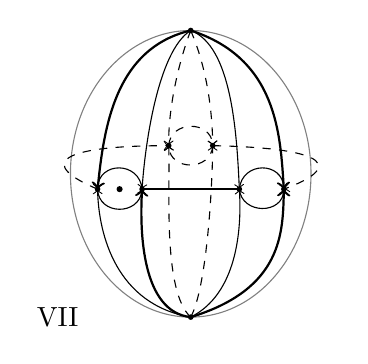
\begin{tikzpicture}[scale=.65]
\draw[gray] (0,0) ellipse (2.35 and 2.8);
\coordinate (P) at (0,2.8);\coordinate (M) at (0,-2.8);
\coordinate (A) at (-1.82,-.3);\coordinate (B) at (-.95,-.3);
\coordinate (C) at (-.43,.55);\coordinate (D) at (.43,.55);
\coordinate (E) at (.95,-.3);\coordinate (F) at (1.82,-.3);
\foreach \p in {P,M,A,B,C,D,E,F}{\fill (\p) circle (.055);}
\draw[thick,->] (P)..controls (-1.5,2.45) and (-1.7,.85)..(A);
\draw[->] (P)..controls (-.65,2.4) and (-.9,.5)..(B);
\draw[dashed,->] (P)..controls (-.25,2.15) and (-.44,1.25)..(C);
\draw[dashed,->] (P)..controls (.3,2.1) and (.42,1.3)..(D);
\draw[->] (P)..controls (.8,2.5) and (.9,.8)..(E);
\draw[thick,->] (P)..controls (1.7,2.25) and (1.75,.75)..(F);
\draw[->] (M)..controls (-1.45,-2.55) and (-1.8,-1.2)..(A);
\draw[thick,->] (M)..controls (-.95,-2.7) and (-1,-1.15)..(B);
\draw[dashed,->] (M)..controls (-.55,-2.3) and (-.4,-.3)..(C);
\draw[dashed,->] (M)..controls (.3,-2.25) and (.42,-.4)..(D);
\draw[->] (M)..controls (.9,-2.35) and (1,-1.1)..(E);
\draw[thick,->] (M)..controls (1.8,-2.25) and (1.8,-1.15)..(F);
\draw[<-] (B)..controls (-1,-.82) and (-1.8,-.82)..(A);
\draw[->] (B)..controls (-1,.25) and (-1.8,.25)..(A);
\draw[dashed,->] (C)..controls (-.4,1.05) and (.4,1.05)..(D);
\draw[dashed,->] (D)..controls (.4,.05) and (-.4,.05)..(C);
\draw[->] (E)..controls (1,.25) and (1.8,.25)..(F);
\draw[->] (E)..controls (1,-.8) and (1.8,-.8)..(F);
\draw[thick] (B)--(E);
\draw[dashed,->] (A)..controls (-3,.2) and (-2.6,.55)..(C);
\draw[dashed,->] (D)..controls (2.85,.5) and (2.9,.1)..(F);
\fill (-1.39,-.3) circle (.06);
\node at (-2.6,-2.8) {$\mathrm{VII}$};
\end{tikzpicture}}
\margin{\uline{NB} les $b_i^\omega$ reliant directement les $\unsure{Q_i|R_i}$ sont ici inutiles}
\figure{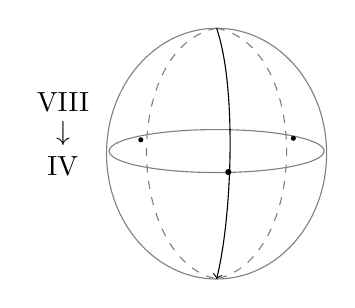
\begin{tikzpicture}[scale=.65]
\draw[gray] (0,0) ellipse (2.15 and 2.45);
\draw[gray] (0,.05) ellipse (2.1 and .42);
\draw[gray,dashed] (0,2.45)..controls (-1.85,2.1) and (-1.8,-2.05)..(0,-2.45);
\draw[gray,dashed] (0,2.45)..controls (1.85,2.1) and (1.8,-2.05)..(0,-2.45);
\draw[->] (0,2.45)..controls (.4,1.3) and (.3,-1.25)..(0,-2.45);
\fill (-1.48,.27) circle (.05);\fill (1.5,.3) circle (.05);\fill (.23,-.36) circle (.06);
\node at (-3,1) {$\mathrm{VIII}$};\node at (-3,.4) {$\unsure{\downarrow}$};\node at (-3,-.25) {$\mathrm{IV}$};
\end{tikzpicture}}
représenté par un graphe un peu plus grand --- dans $\boxed{\mathrm{VIII}}$ on distingue les \inserted{six} \deleted{flèches} $d_i^\omega$ seulement, et on en donne \unsure{par} en plus les $\widetilde a_i^\omega$, ce qui est inutile en fait par (35). (Donc il n'est pas étonnant que dans (37), la donnée de $\widetilde\alpha$, qui
\margin{37}

\scanpage{39}
\mspage{20}
repère \inserted{les} $u(\widetilde a_i^\omega)$, résulte déjà de celle de $\xi$, qui repère \inserted{les} $u(d_i^\omega)$,
\figure{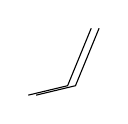
\begin{tikzpicture}[baseline=0pt]\draw (0,0)--(.5,.12)--(.8,.85);\draw (.1,0)--(.6,.12)--(.9,.85);\end{tikzpicture}}
Les graphes $\mathrm{I}$ à $\mathrm{VII}$ donnent lieu au diagramme d'inclusions
\diagram{\begin{tikzcd}[ampersand replacement=\&,column sep=2em,row sep=2.8em,execute at end picture={\draw ([xshift=-4mm,yshift=5mm]\tikzcdmatrixname-2-1.north west) rectangle ([xshift=5mm,yshift=-4mm]\tikzcdmatrixname-3-3.south east);}]
\&\&\mathrm{III}\arrow[dl,hook]\arrow[dr,hook]\&\&\\
\mathrm{I}\arrow[r,hook]\arrow[dr,hook]\&\mathrm{II}\arrow[dr,hook]\arrow[r,draw=none,"\unsure{\deleted{\leftrightarrow}|\leftrightarrow}"]\&\phantom{\mathrm{II}}\&\mathrm{IV}\arrow[dl,hook]\&\mathrm{V}\arrow[l,hook]\\
\&\mathrm{VII}\arrow[r,hook]\&\mathrm{VI}\&\&
\end{tikzcd}}\quad(68)

Sans calcul, je peux déjà prédire que la donnée d'un autom. de $\mathrm{VII}$ fixant les sommets et commutant à $\unsure{\mathcal G_J|G_J}$, équivaut à la donnée des quantités
\[
(69)\qquad (\uline{\lambda},\beta',\uline{\xi'})\in\widehat\Pi_{0,3}\times\widehat\Pi_{0,3}\times\widehat\Pi_{0,3}
\]
reliés par \deleted{\unsure{les}} \unsure{l'|les} équations \deleted{(63) ici}
\[
(70)\qquad\left\{\begin{aligned}
\beta'&=\alpha'\sigma_\infty(\lambda)\\
\beta'\sigma_\infty(\beta')&=1
\end{aligned}\right.\qquad
\begin{gathered}
\text{où}\quad\alpha'=\xi'\rho^{\unsure{\phantom{-1}|-1}}(\xi')^{-1}\\
\text{i.e.}\quad\alpha'\sigma_\infty(\lambda)\sigma_\infty(\alpha')\lambda=1
\end{gathered}
\]
\margin{\figure{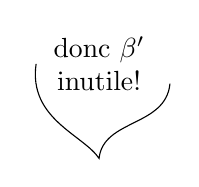
\begin{tikzpicture}\node[align=center] at (0,.6) {donc $\beta'$\\inutile!};\draw (-.8,.6)..controls (-.9,-.1) and (-.2,-.3)..(0,-.6)..controls (.05,-.1) and (.85,-.2)..(.9,.35);\end{tikzpicture}}}
(\unsure{tout|tandis} comme \inserted{dans le cas où} $\mathrm{II}$ est défini par \deleted{$(\lambda,\eta,\alpha')$},
\deleted{reliés par}
\[
(69')\qquad(\uline{\lambda},\uline{\eta},\alpha')\in\widehat\Pi_{0,3}\times\widehat\Pi_{0,3}\times\widehat\Pi_{0,3}
\]
avec \unsure{l'|les} équations
\[
(70')\qquad\left\{\begin{aligned}
\beta'&=\alpha'\sigma_\infty(\lambda)\\
\alpha'\rho(\alpha')\rho^2(\alpha')&=1
\end{aligned}\right.\qquad\text{où}\quad\beta'=\eta\sigma_\infty(\eta)^{-1}
\]
\margin{donc $\alpha'$ inutile!}
\margin{38}

\scanpage{40}
\mspage{21}
Je vais expliciter les calculs dans le groupoïde $\mathrm{VII}$, associé au graphe de $=$ nom, on a des flèches génératrices
\[
(71)\qquad\left\{\begin{aligned}
\widetilde d_i^\omega&:P^\omega\longrightarrow R_i^\omega\\
\widetilde d_i^{\prime\omega}&:P^\omega\longrightarrow R_i^{\omega'}\\
a_i^\omega&:R_i^\omega\mathbin{-}R_i^{\omega'}
\end{aligned}\right.
\]
liées par les relations
\[
(72)\qquad\left\{\begin{aligned}
(\widetilde d_i^{\unsure{\omega\prime|\prime\omega}})^{-1}a_i^\omega\widetilde d_i^\omega&=1\\
(d_{\omega i}^{\prime\omega})^{-1}\widetilde d_{\omega i}^{\omega'}(d_i^{\prime\omega'})^{-1}\widetilde d_i^\omega&=1
\end{aligned}\right.
\]
\margin{six relations indépendantes exprimant les $\widetilde d_i^{\prime\omega}$ en termes des $\widetilde d_i^\omega$ et $a_i^\omega$, \inserted{ou les $\unsure{a_i^\omega}$ en termes des $\widetilde d_i^\omega,\widetilde d_i^{\prime\omega}$.}}
\margin{en apparence six relations, mais il n'y en a que trois indépendantes, car l'équation pour $i,\omega$ et pour $(\unsure{\omega i|i},\omega')$ est la $=$.}
\figure{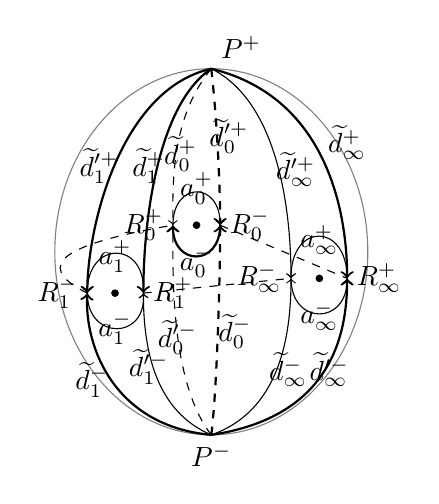
\begin{tikzpicture}[scale=.75]
\draw[gray] (0,0) ellipse (2.65 and 3.1);
\coordinate (P) at (0,3.1);\coordinate (M) at (0,-3.1);
\coordinate (L1) at (-2.1,-.7);\coordinate (R1) at (-1.15,-.7);
\coordinate (L0) at (-.65,.45);\coordinate (R0) at (.15,.45);
\coordinate (LI) at (1.35,-.45);\coordinate (RI) at (2.3,-.45);
\draw[dashed] (L1)..controls (-3.1,-.2) and (-2.4,.15)..(L0);
\draw[dashed] (R0)--(RI);\draw[dashed] (R1)--(LI);
\fill (-1.63,-.7) circle (.065);\fill (-.25,.45) circle (.065);\fill (1.83,-.45) circle (.065);
\draw[->,thick] (P)..controls (-1.55,2.75) and (-2.1,.4)..(L1);
\draw[->,thick] (P)..controls (-.9,2.5) and (-1.15,.55)..(R1);
\draw[dashed,->] (P)..controls (-.7,2.25) and (-.65,1.1)..(L0);
\draw[dashed,->,thick] (P)..controls (.1,2.2) and (.15,1.1)..(R0);
\draw[->] (P)..controls (1.2,2.5) and (1.35,.5)..(LI);
\draw[->,thick] (P)..controls (2.05,2.6) and (2.3,.5)..(RI);
\draw[->,thick] (M)..controls (-1.65,-2.95) and (-2.15,-1.6)..(L1);
\draw[->] (M)..controls (-.95,-2.7) and (-1.15,-1.65)..(R1);
\draw[dashed,->] (M)..controls (-.7,-2.2) and (-.65,-.35)..(L0);
\draw[dashed,->,thick] (M)..controls (.1,-2.3) and (.15,-.35)..(R0);
\draw[->] (M)..controls (1.15,-2.7) and (1.35,-1.45)..(LI);
\draw[->,thick] (M)..controls (2,-2.8) and (2.3,-1.45)..(RI);
\draw[->] (R1)..controls (-1.1,.2) and (-2.1,.2)..(L1);
\draw[->] (L1)..controls (-2.1,-1.5) and (-1.1,-1.5)..(R1);
\draw[->] (L0)..controls (-.65,1.2) and (.15,1.2)..(R0);
\draw[->,thick] (R0)..controls (.15,-.25) and (-.65,-.25)..(L0);
\draw[->] (RI)..controls (2.3,.5) and (1.35,.5)..(LI);
\draw[->] (LI)..controls (1.35,-1.25) and (2.3,-1.25)..(RI);
\node[above right] at (P) {$P^+$};\node[below] at (M) {$P^-$};
\node[left] at (L1) {$R_1^-$};\node[right] at (R1) {$R_1^+$};
\node[left] at (L0) {$R_0^+$};\node[right] at (R0) {$R_0^-$};
\node[left] at (LI) {$R_\infty^-$};\node[right] at (RI) {$R_\infty^+$};
\node at (-1.63,-.08) {$a_1^+$};\node at (-1.63,-1.3) {$a_1^-$};
\node at (-.25,1.07) {$a_0^+$};\node at (-.25,-.17) {$a_0^-$};
\node at (1.83,.2) {$a_\infty^+$};\node at (1.83,-1.08) {$a_\infty^-$};
\node at (-1.9,1.45) {$\widetilde d_1^{\prime+}$};\node at (-1.06,1.45) {$\widetilde d_1^+$};
\node at (-.52,1.65) {$\widetilde d_0^+$};\node at (.3,1.95) {$\widetilde d_0^{\prime+}$};
\node at (1.43,1.4) {$\widetilde d_\infty^{\prime+}$};\node at (2.3,1.85) {$\widetilde d_\infty^+$};
\node at (-2.02,-2.17) {$\widetilde d_1^-$};\node at (-1.06,-1.95) {$\widetilde d_1^{\prime-}$};
\node at (-.57,-1.45) {$\widetilde d_0^{\prime-}$};\node at (.4,-1.35) {$\widetilde d_0^-$};
\node at (1.3,-2) {$\widetilde d_\infty^-$};\node at (2,-2) {$\widetilde d_\infty^{\prime-}$};
\end{tikzpicture}}
On va repérer $u$ par les équations
\[
(73)\qquad\left\{\begin{aligned}
u(\widetilde d_i^\omega)&=\deleted{\unsure{\widetilde d_i^\omega}}\varphi_i^\omega(\xi_1^{\deleted{\unsure{'}}})\widetilde d_i^\omega\\
u(\widetilde d_i^{\prime\omega})&=\deleted{\unsure{\widetilde d_i^{\prime\omega}}}\varphi_i^{\omega'}(\xi')\widetilde d_i^{\prime\omega}\\
u(a_i^\omega)&=a_i^\omega\varphi_i^\omega(\lambda)
\end{aligned}\right.\qquad \xi',\xi_1^{\deleted{\unsure{'}}},\lambda\in\widehat\Pi_{0,3}
\]
et il reste à exprimer que $u$ satisfait les relations (72). La première s'explicite sous la forme
\[
(74)\qquad\xi'=\varepsilon_0(\lambda\xi_1)\qquad\text{i.e.}\quad\xi_1=\lambda^{-1}\cdot\varepsilon_0^{-1}(\xi')
\]
et on trouve également
\[
(75)\qquad\deleted{\unsure{\beta}}\xi_1=\beta'\sigma_\infty(\xi')
\]
\margin{où $\beta'$ défini par la condition $(\unsure{65\,a|65\,'})$}
Cette \unsure{relation|relations} permettant de tirer $\beta'$ en termes
\margin{39}

\scanpage{41}
\mspage{22}
de $\xi',\xi_1$ ou de l'une de ces quantités seulement
\[
(\unsure{76|75})\qquad\begin{aligned}
\beta'&=\xi_1\sigma_\infty(\xi')^{-1}=\deleted{\varepsilon_0(\lambda\xi_1)}\xi_1(\sigma_\infty\varepsilon_0)(\lambda\xi_1)^{-1}\\
&=\lambda^{-1}\cdot\varepsilon_0^{-1}(\xi')\sigma_\infty(\xi')^{-1}.
\end{aligned}
\]
de \deleted{la dernière} \inserted{ces} expressions de $\beta'$ on tire
\[
(\unsure{76'|75'})\qquad\begin{aligned}
\sigma_\infty(\beta')&=\sigma_\infty(\xi_1)\xi'^{-1}=\sigma_\infty(\xi_1)\varepsilon_0(\lambda\xi_1)^{-1}\\
&=\sigma_\infty(\lambda)^{-1}\underbrace{\overbrace{\rho(\xi')\xi'^{-1}}^{\alpha'^{-1}}}_{\deleted{\unsure{\alpha'}}}
\end{aligned}
\]
et la troisième expression de $\beta'$ \deleted{donne}

\deleted{$(\unsure{77})$ \unsure{Ceci|Ce} dit, l'équation que $(72\,b)$ équivaut à:}
\deleted{\[(\unsure{77})\qquad\beta'\sigma_\infty(\beta')=1\]}
\deleted{soit, $\sigma_\infty(\beta')$ en posant $\beta_1=\sigma_\infty(\beta')$, \unsure{pour}}
\figure{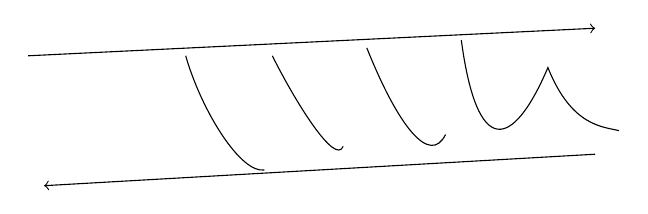
\begin{tikzpicture}[x=1cm,y=1cm]\draw[->] (0,1)--(7.2,1.35);\draw[->] (7.2,-.25)--(.2,-.65);\draw (2,1)..controls (2.2,.3) and (2.7,-.5)..(3,-.45);\draw (3.1,1)..controls (3.4,.4) and (3.9,-.4)..(4,-.15);\draw (4.3,1.1)..controls (4.7,.1) and (5.1,-.4)..(5.3,0);\draw (5.5,1.2)..controls (5.7,-.3) and (6.15,-.2)..(6.6,.85)..controls (6.9,.1) and (7.3,.1)..(7.5,.05);\end{tikzpicture}}
s'écrit aussi
\[
(77)\qquad\sigma_\infty(\beta')^{-1}=\alpha'\sigma_\infty(\lambda).
\]
Ceci posé, l'équation $(72\,b)$ équivaut à
\[
(78)\qquad\beta'\sigma_\infty(\beta')=1\qquad\text{ou encore}\quad\sigma_\infty(\beta')^{-1}=\beta'
\]
ce qui est invariant par la substitution $\beta'\mapsto\sigma_\infty(\beta')$ ou $\beta'\mapsto\beta'^{-1}$, donc posant
\inserted{\unsure{ces|ceci}\ \unsure{signes|suppose}\ \unsure{n'ont pas|implique}}
\[
(*)\qquad\beta_1=\sigma_\infty(\beta')^{-1}=\alpha'\sigma_\infty(\lambda)
\]
l'équation (78) équivaut à l'équation
\[
(**)\qquad\beta_1\sigma_\infty(\beta_1)=1
\]
et implique que $\beta_1=\sigma_\infty(\beta_1)^{-1}$ donc $\beta_1=\beta'$.

En résumé, on peut donc de suite poser
\[
(79)\qquad\beta'=\alpha'\sigma_\infty(\lambda)\qquad\text{où}\quad\alpha'=\xi'\rho(\xi')^{-1}
\]
et la relation à imposer à $(\lambda,\xi')$ est, au choix,
\margin{40}

\scanpage{42}
\mspage{23}
l'égalité \unsure{du|de} $\beta'$ défini par cette équation avec celui défini par \inserted{les formules équivalentes} $(\unsure{76|75})$ ou $(\unsure{76'|75'})$ ou (77), ou

\deleted{le fait que $\beta'$ \unsure{(ce}}
l'équation (78), écrite au choix pour $\beta'$ défini par l'une des formules $(\unsure{76|75})$ à (77), ou par la formule (79) --- ce qui donne la formulation la plus simple.
\margin{41}

\scanpage{44}
\margin{43}
\mspage{1}
\margin{Attention, notations \unsure{de ce qui suit} p.r. à celles des calculs précédents, en $\alpha,\beta,\alpha',\beta',\xi,\eta,\xi'\ldots$}
Considérons une 2-sphère conforme \inserted{$\Sigma$} avec une partie $J$ à trois éléments,
\[
(1)\qquad J\subset\Sigma,\qquad J=(R_i)_{i\in J}
\]
de sorte que le groupe $\unsure{\mathcal G_J|G_J}$ opère sur $\Sigma$ par automorphismes \deleted{orientés} directs, \deleted{et que} \deleted{$\unsure{G'_J|G_J}\times\{1,\tau\}$ le groupe des} \inserted{tandis que le groupe des automorphismes} conformes de la situation $(\Sigma,J)$ est
\[
(2)\qquad\Gamma_{\Sigma,J}=\Gamma\simeq\unsure{\mathcal G_J|G_J}\times\{1,\tau\}
\]
\margin{\uline{NB} L'antipodisme ne fait \uline{pas} partie de $\Gamma$, car il ne stabilise pas $J$}
$\tau$ est l'unique \deleted{anti} autom. $\unsure{+|\ne}1$ \deleted{\unsure{qui est}} qui fixe les $R_i$ \deleted{\unsure{tous}} ($\tau={}$conjugaison complexe).
\margin{donc la \unsure{catégorie des} $(\Sigma,J)$ équiv. à celle des couples $(J,\uline{\bar\omega})$, où $J\in(\mathrm{Ens})_3$ et $\uline{\bar\omega}\in(\mathrm{Ens})_2$ cf plus bas}
Il y a sur $\Sigma$ une unique métrique riemannienne homogène \unsure{invariante|invariant} pour $\unsure{\mathcal G_J|G_J}$, \inserted{à scalaire $\lambda\in\mathbb R^{++}$ près} \deleted{pour laquelle}, qui nous permet d'identifier canoniquement $\Sigma$ à la sphère unité dans un espace vectoriel réel euclidien $E_{\unsure{3}}$. On pose
\[
(3)\qquad\left\{\begin{aligned}
\uline{\bar\omega}&=\Omega(\Sigma)\simeq\Omega(E_{\unsure{3}})\\
\uline{\omega}&=\Omega(J)\simeq\Omega(\Sigma_{\mathbb R})\\
\uline{\varepsilon}&=\Pi_0(\Sigma\setminus\Sigma_{\mathbb R})=\Pi_0(E\setminus\unsure{V|\forall})=\Pi_0((E/V)^*)
\end{aligned}\right.
\]
\margin{ens des deux orientations de $\Sigma$, ou donc de $E$}
\margin{On pourrait écrire $E(J,\uline{\bar\omega})$ $V(J,\uline{\omega})$.}
\margin{On a
\[
\uline{\omega}\wedge\uline{\varepsilon}\wedge\uline{\bar\omega}=1
\]
i.e.
\[
(3\text{ bis})\qquad\left\{\begin{aligned}
\uline{\omega}&\simeq\uline{\varepsilon}\wedge\uline{\bar\omega}\\
\uline{\varepsilon}&\simeq\uline{\bar\omega}\wedge\uline{\omega}\\
\uline{\bar\omega}&\simeq\uline{\omega}\wedge\uline{\varepsilon}
\end{aligned}\right.
\]
par la conv. de \unsure{Stokes entre} orientations d'un hémisphère et celles de \unsure{son|leur} bord, \unsure{plus précis (4) ici}}
$V$ est le \inserted{$\mathbb R$-}sous-espace vectoriel de $E$ \uline{engendré} par les $R_{\unsure{J|i}}$, qui est de dimension 2, et où
\[
(4)\qquad\Sigma_{\mathbb R}=\Sigma\cap V
\]
cercle euclidien \unsure{ds le|dans le} plan euclidien $V$

\scanpage{45}
On aura dans $V$
\[
(4)\qquad\sum_{j\in J}R_j=0
\]
ce qui donne un isomorphisme
\[
(5)\qquad V\simeq V_J(\mathbb R)=\operatorname{Ker}(\mathbb R^J\xrightarrow[\text{somme}]{}\mathbb R)
\]
et on a, par la $3^{\unsure{\text{ième}|\text{ème}}}$ formule (3)
\[
(6)\qquad\Delta=V^\perp\simeq\mathbb R(\varepsilon)
\]
\margin{``axe polair''}
\margin{orth. de $V$ dans $E$}
\margin{(isom compatible avec la structure quadratique)}
donc
\[
(7)\qquad E\simeq V_J(\mathbb R)\oplus\mathbb R(\varepsilon)
\]
\margin{isom d'espaces euclidiens}
où dans $V_J(\mathbb R)$ on prend la seule forme quadratique \inserted{$q$} pour laquelle les $R_j$ \deleted{sont} \inserted{satisfont} \deleted{de carré \unsure{un}}
\[
q(R_j)=1
\]
\margin{Il est clair, par cette caractérisation de $q$, que l'opération naturelle de $\unsure{\mathcal G_J|G_J}$ sur $V(J)$ conserve $q$.}
\unsure{(prenant|(prendre} une base formée de $R_i,R_j$, $R_{\unsure{n|h}}$ de coordonnées $(-1,-1)$, la forme quadratique en question est $x^2-xy+y^2$)

Dans le plan euclidien $V$, les $R_i$ \figure{\begin{tikzpicture}[baseline=0pt]\draw[->] (.3,.55)--(0,.35)--(0,0);\end{tikzpicture}} forment les sommets d'un triangle équilatéral inscrit dans le cercle unité. L'opération de $\unsure{\mathcal G_J|G_J}$ sur $E$ se fait par son opération \deleted{sur} tautologique sur $V(J)$ et l'opération par $\operatorname{sg}(g)$ sur $\Delta$:
\margin{44}

\scanpage{46}
\mspage{2}
\[
(8)\qquad g_E=\underbrace{g_{V_J(\mathbb R)}}_{\text{tautol.}}\oplus\operatorname{sg}(g)\operatorname{id}_\Delta
\]
L'opération de $\tau$ est donnée par
\[
(9)\qquad\tau_E=\operatorname{id}_{V_J(\mathbb R)}\oplus(-\operatorname{id}_\Delta)
\]
Je pose
\[
(10)\qquad\Sigma^*=\Sigma\setminus J=\Sigma-\{R_{\deleted{\unsure{j}}\inserted{i}}\mid i\in I\}
\]
et je m'intéresse au groupoïde fondamental de $\Sigma^*$, comme exercice préliminaire de syntaxe galoisienne, avant de regarder des situations \inserted{un peu} plus complexes (le triangle équilatéral remplacé par d'autres configurations riches en symétries sur la sphère, voire sur d'autres surfaces que la sphère, ou celle-ci étant remplacée par le fibré de Hopf, en vue des applications au calcul des groupoïdes de Teichmüller...).

Il est commode d'introduire une compactification de $\Sigma^*$, pour disposer ainsi de ``pts-base'' ``proches'' \unsure{desdits} $R_i$.
\margin{45}

\scanpage{47}
\margin{La construction de l'éclaté marche dans le contexte des variétés $C^\infty$ et \unsure{des variétés} d'ailleurs analytiques réelles.}
Pour ceci, considérons l'éclaté réel de $\Sigma$ en $J$, soit $\Sigma'$, dans lequel l'image inverse de $i\in J$ s'identifie à: \deleted{$\unsure{P(}$ l'espace} la droite projective réelle
\[
(11)\qquad\Sigma'_{R_i}\simeq P(\underbrace{T_{\Sigma,R_i}})
\]
\margin{\unsure{esp.|espace} tangent à $\Sigma$ en $R_i$, identifié à: $T_{\Sigma,R_i}^*/\mathbb R^*$}
qui est un cercle plongé dans la surface compacte $\Sigma'$ (qu'on peut considérer comme \unsure{obtenu|obtenue} en enlevant de la sphère trois rondelles autour des $R_i$, et y recollant des rubans de Möbius --- on obtient une surface non \uline{orientable} dont le \deleted{genre} $\chi_!$ est égal à
\[
\begin{aligned}
&\chi_!(\Sigma)\deleted{\unsure{-3}}\inserted{-3\chi_!(\text{rondelle ouverte})}+3(\underbrace{\chi_!(\text{ruban Möbius})}_{0}\\
&\deleted{\unsure{\text{à}}}=2-3=-1=1-g,
\end{aligned}
\]
donc le genre est $2$).

La découpe de cette surface suivant $\bigcup\Sigma'_{R_i}$ est une surface à bord compacte, \deleted{dont} \inserted{en fait} soit $\widetilde\Sigma$, avec
\margin{$\partial\widetilde\Sigma$ un rev. double de $\coprod_i\Sigma'_{R_i}$}
\[
(12)\qquad\partial\widetilde\Sigma\simeq\coprod_{i\in I}\underbrace{TU_{\Sigma,R_i}}
\]
\margin{cercle tangent à $\Sigma$ en $R_i$, identifiable à $T_{\Sigma,R_i}^*/\mathbb R^{*+}$ noté aussi $U_i$}
\margin{$\widetilde\Sigma$ est une sphère à bord à trois trous. Notons que $\widetilde\Sigma^\circ$ a une structure conforme, mais que celle-ci ne se prolonge pas à $\widetilde\Sigma$.}
\margin{46}

\scanpage{48}
\mspage{3}
On a \unsure{les|des} équivalences de catégories
\diagram{
\begin{tikzcd}[ampersand replacement=\&]
(13)\quad \operatorname{Rev\,\text{ét}}(\widetilde\Sigma) \arrow[r,"\approx","\text{équiv.}"'] \& \operatorname{Rev\,\text{ét}}(\widetilde\Sigma^\circ) \arrow[r,"\sim","\text{iso}"'] \& \operatorname{Rev\,\text{ét}}(\Sigma^*)
\end{tikzcd}
}
déduites de l'inclusion
\[
\widetilde\Sigma^\circ \overset{\mathrm{def}}= \widetilde\Sigma\setminus\unsure{\partial|\delta}\widetilde\Sigma = \widetilde\Sigma|\Sigma^* \hookrightarrow \widetilde\Sigma
\]
et de l'isomorphisme
\[
\widetilde\Sigma^\circ \xrightarrow{\sim} \Sigma^*,
\]
d'où une équivalence entre les groupoïdes fondamentaux au sens large (\unsure{dt|dont} les objets sont les rev. étales 1-connexes)\deleted{\unsure{des}}
\[
(14)\qquad \Pi_1(\widetilde\Sigma) \longrightarrow \Pi_1(\Sigma^*)
\]
et en composant avec
\[
\Pi_1(U_i)\longrightarrow \Pi_1(\widetilde\Sigma)
\]
déduit de l'inclusion $U_i\hookrightarrow\widetilde\Sigma$, on trouve
\[
(15)\qquad \Pi_1(\deleted{\unsure{\Sigma}}U_i)\longrightarrow\Pi_1(\Sigma^*).
\]
Nous allons représenter graphiquement l'homomorphisme 14, en ``dessinant'' $\widetilde\Sigma$ sur $\Sigma^*$, comme une région qui serait contenue dans $\Sigma^*$ en lui enlevant \inserted{l'intérieur de} trois disques \inserted{fictifs} $\unsure{\Delta_i}$ ``infiniment petits'' \deleted{et} (s'identifiant aux disques ouverts des $T_{\Sigma,R_i}$ \deleted{\unsure{g}}, ou encore aux cônes sur les $U_i$), et on se représente (14) comme provenant d'une telle inclusion fictive.
\margin{Plus précisément au lieu de travailler sur $\Sigma^*$, nous travaillons sur $C$ \unsure{``sphère à trous''} un peu plus grande que $\widetilde\Sigma$.}
\margin{47}

\scanpage{49}
En fait, nous allons travailler avec des éléments de $\Pi_1(\widetilde\Sigma)$ qui proviennent, soit des p\textsuperscript{ts} de $\widetilde\Sigma$, donc des p\textsuperscript{ts} de $\Sigma^*$ ou d'un des $U_i$, soit des \uline{parties} de $\widetilde\Sigma$ qui sont 1-connexes pour la top. induite par $\widetilde\Sigma$ -- en pratique peut-être des parties \inserted{1-conn.} de $\Sigma^*$, et en les faisant ``déborder'' sur $\widetilde\Sigma$ de façon naturelle.

Le groupe $\Gamma$ opère sur la situation \inserted{$C^\infty$} $(\Sigma,\unsure{J|I})$, donc par transport de structure sur la situation
\[
\widetilde\Sigma\longrightarrow\Sigma,\quad \unsure{J|I}\subset\Sigma
\]
donc sur \deleted{\unsure{le}} (14) (15). Un aspect essentiel du travail à faire est de garder \deleted{\unsure{cette}} constamment présente à l'esprit cette opération, et d'introduire des \unsure{notions|notations} et des constructions qui soient invariantes, dans le sens requis par la situation, par les opérations en question.
\margin{48}

\scanpage{50}
\mspage{4}
\figure{
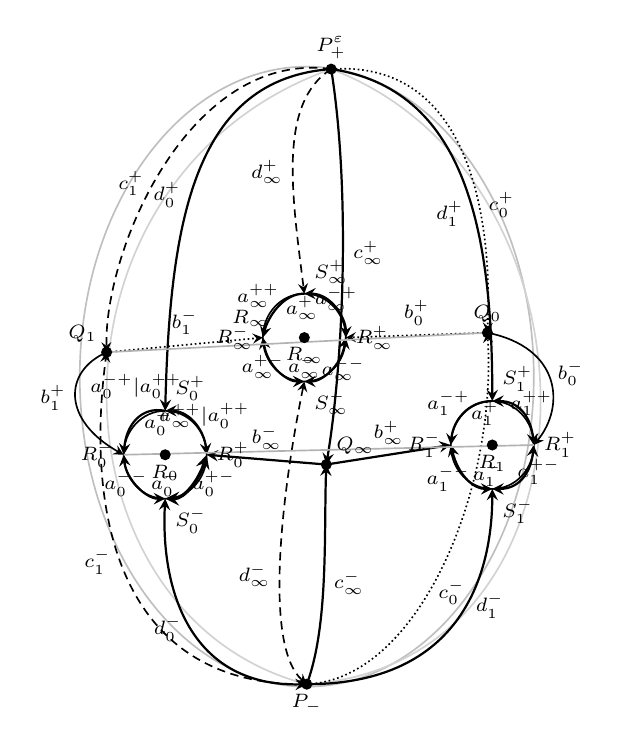
\begin{tikzpicture}[x=.62cm,y=.62cm,>=stealth,every node/.style={font=\scriptsize},line width=.6pt]
\coordinate (Pp) at (5.2,13.2); \coordinate (Pm) at (4.7,.6);
\coordinate (Qz) at (8.4,7.8); \coordinate (Qo) at (.6,7.4); \coordinate (Qi) at (5.1,5.1);
\coordinate (Rz) at (1.8,5.3); \coordinate (Ro) at (8.5,5.5); \coordinate (Ri) at (4.65,7.7);
\draw[gray!50] (4.7,6.9) ellipse (4.65 and 6.35);
\draw[gray!35] (Pp) .. controls (-1,11) and (-.7,2) .. (Pm) .. controls (11,1) and (11,11) .. (Pp);
\draw[densely dashed,->] (Pp) .. controls (2.3,13.6) and (.55,9.5) .. (Qo) node[pos=.55,left] {$c_1^+$};
\draw[densely dashed,->] (Pm) .. controls (.9,.55) and (.15,4) .. (Qo) node[pos=.55,left] {$c_1^-$};
\draw[densely dotted,->] (Pp) .. controls (8.1,13.4) and (8.5,10) .. (Qz) node[pos=.64,right] {$c_0^+$};
\draw[densely dotted,->] (Pm) .. controls (7,.7) and (8.6,4.6) .. (Qz) node[pos=.43,right] {$c_0^-$};
\draw[thick,->] (Pp) .. controls (5.6,10.7) and (5.45,7.2) .. (Qi) node[pos=.45,right] {$c_\infty^+$};
\draw[thick,->] (Pm) .. controls (5.15,1.8) and (5.05,3.7) .. (Qi) node[pos=.48,right] {$c_\infty^-$};
\draw[thick,->] (Pp) .. controls (2.4,13.0) and (1.9,10.1) .. (1.8,6.2) node[pos=.56,left] {$d_0^+$};
\draw[thick,->] (Pp) .. controls (7.9,12.8) and (8.5,10) .. (8.5,6.4) node[pos=.6,left] {$d_1^+$};
\draw[densely dashed,->] (Pp) .. controls (4.1,12.5) and (4.4,10.6) .. (4.65,8.6) node[pos=.56,left] {$d_\infty^+$};
\draw[thick,<->] (Pm) .. controls (2.4,.55) and (1.7,2.4) .. (1.8,4.4) node[pos=.5,left] {$d_0^-$};
\draw[thick,->] (Pm) .. controls (7.9,.6) and (8.5,2.9) .. (8.5,4.6) node[pos=.55,right] {$d_1^-$};
\draw[densely dashed,<->] (4.65,6.8) .. controls (4.2,4.6) and (3.8,1.4) .. (Pm) node[pos=.55,left] {$d_\infty^-$};
\draw[->,densely dotted] (Qo)--(3.8,7.7) node[midway,above] {$b_1^-$};
\draw[->,densely dotted] (Qz)--(5.5,7.7) node[midway,above] {$b_0^+$};
\draw[thick,->] (Qi)--(2.65,5.3) node[midway,above] {$b_\infty^-$};
\draw[thick,->] (Qi)--(7.65,5.5) node[midway,above] {$b_\infty^+$};
\draw[->] (Qo) .. controls (-.3,7) and (-.3,6) .. (.95,5.3) node[pos=.5,left] {$b_1^+$};
\draw[->] (Qz) .. controls (9.9,7.5) and (10,6.3) .. (9.35,5.5) node[pos=.45,right] {$b_0^-$};
\draw (Rz) ellipse (.85 and .9); \draw (Ro) ellipse (.85 and .9); \draw (Ri) ellipse (.85 and .9);
\draw[->,thick] (1.8,6.2) .. controls (1.3,6.3) and (1,5.9) .. (.95,5.3);
\draw[<->,thick] (1.8,6.2) .. controls (2.3,6.2) and (2.6,5.8) .. (2.65,5.3);
\draw[<->,thick] (.95,5.3) .. controls (1,4.8) and (1.4,4.4) .. (1.8,4.4);
\draw[<->,very thick] (2.65,5.3) .. controls (2.5,4.8) and (2.2,4.4) .. (1.8,4.4);
\draw[->,thick] (8.5,6.4) .. controls (8,6.4) and (7.7,6) .. (7.65,5.5);
\draw[<->,thick] (8.5,6.4) .. controls (9.1,6.4) and (9.3,6) .. (9.35,5.5);
\draw[<->,thick] (7.65,5.5) .. controls (7.8,4.9) and (8.1,4.6) .. (8.5,4.6);
\draw[<->,thick] (8.5,4.6) .. controls (9.1,4.6) and (9.3,5) .. (9.35,5.5);
\draw[->,thick] (4.65,8.6) .. controls (4.2,8.6) and (3.9,8.1) .. (3.8,7.7);
\draw[<->,thick] (4.65,8.6) .. controls (5.2,8.6) and (5.5,8.1) .. (5.5,7.7);
\draw[<->,thick] (3.8,7.7) .. controls (3.9,7.1) and (4.3,6.8) .. (4.65,6.8);
\draw[<->,thick] (5.5,7.7) .. controls (5.4,7.1) and (5,6.8) .. (4.65,6.8);
\draw[gray!60] (Qo)--(Qz) (.95,5.3)--(9.35,5.5);
\foreach \p in {Pp,Pm,Qz,Qo,Qi,Rz,Ro,Ri} \fill (\p) circle (2pt);
\node[above] at (Pp) {$P_{+}^{\deleted{\unsure{\varepsilon}}}$}; \node[below] at (Pm) {$P_-$};
\node[above left] at (Qo) {$Q_1$}; \node[above] at (Qz) {$Q_0$}; \node[above right] at (Qi) {$Q_\infty$};
\node[below] at (Rz) {$R_0$}; \node[below] at (Ro) {$R_1$}; \node[below] at (Ri) {$R_\infty$};
\node[left] at (.95,5.3) {$R_0^-$}; \node[right] at (2.65,5.3) {$R_0^+$};
\node[left] at (7.65,5.5) {$R_1^-$}; \node[right] at (9.35,5.5) {$R_1^+$};
\node[left] at (3.8,7.7) {$R_\infty^-$}; \node[right] at (5.5,7.7) {$R_\infty^+$};
\node[above right] at (1.8,6.2) {$S_0^+$}; \node[below right] at (1.8,4.4) {$S_0^-$};
\node[above right] at (8.5,6.4) {$S_1^+$}; \node[below right] at (8.5,4.6) {$S_1^-$};
\node[above right] at (4.65,8.6) {$S_\infty^+$}; \node[below right] at (4.65,6.8) {$S_\infty^-$};
\node at (1.2,6.7) {$\unsure{a_0^{-+}|a_0^{++}}$}; \node at (2.6,6.1) {$\unsure{a_\infty^{++}|a_0^{++}}$};
\node at (2.8,4.7) {$\unsure{a_0^{+-}}$}; \node at (1,4.7) {$\unsure{a_0^{--}}$};
\node at (1.65,5.95) {$a_0^+$}; \node at (1.8,4.7) {$a_0^-$};
\node at (7.6,6.35) {$\unsure{a_1^{-+}}$}; \node at (9.3,6.35) {$a_1^{++}$};
\node at (9.45,4.95) {$\unsure{a_1^{+-}}$}; \node at (7.6,4.8) {$a_1^{--}$};
\node at (8.35,6.15) {$a_1^+$}; \node at (8.4,4.9) {$\unsure{a_1^-}$};
\node at (3.7,8.55) {$a_\infty^{++}$}; \node at (5.3,8.5) {$\unsure{a_\infty^{-+}}$};
\node at (5.45,7.05) {$a_\infty^{--}$}; \node at (3.8,7.1) {$\unsure{a_\infty^{+-}}$};
\node at (4.6,8.3) {$a_\infty^+$}; \node at (4.65,7.1) {$a_\infty^-$};
\node at (3.55,8.1) {$\deleted{\unsure{R_\infty}}$};
\end{tikzpicture}
}
On introduit
\[
(16)\quad\left\{\begin{array}{l}
Q_i\ (i\in\unsure{J|I})\text{ antipodique de }R_i\ \inserted{(=-R_i)}\\
R_i^\omega\in U_i\quad(i\in\unsure{J|I},\omega\in\uline{\omega})\\
P_\varepsilon\ \deleted{\unsure{\in}}\quad(\varepsilon\in\uline{\varepsilon}=\unsure{\pi_0|\Pi_0}(\Sigma\setminus\Sigma_{\mathbb R}))\\
S_i^\varepsilon
\end{array}\right.
\]
où $P_\varepsilon$ est défini par
\[
(17)\qquad\{P_\varepsilon\}=\Delta\cap(\Sigma-\Sigma_{\mathbb R})_\varepsilon
\]
\deleted{\unsure{des} $R_i^\omega\in U_{i\mathbb R}\unsure{\simeq\omega}$}
et $\unsure{R_{i\omega}|R_i^\omega}$ est défini ainsi

On a une bijection canonique
\[
(18)\qquad U_{i\mathbb R}\overset{\mathrm{def}}=\underbrace{U_i\cap\overline T_{\Sigma_{\mathbb R},R_i}}_{T^U_{\Sigma_{\mathbb R},R_i}}\simeq\omega
\]
\unsure{sur} \deleted{\unsure{cette}} variété \inserted{$\Sigma_{\mathbb R}$} de dim 1, l'une des orientations de celle-ci en les points $R_i$ (donc globalement) est en corr. biunivoque avec l'une des deux directions orientées tangentes.
\margin{
\[
(19)\quad S_i^\varepsilon\in U_i\cap\overline T\Sigma_i=T^U\Sigma_i\ \deleted{\unsure{de}}
\]
où $\Sigma_i$ est le grand cercle déterminé par les $P_\varepsilon$ et $Q_i$; on a $T^U\Sigma_i\simeq\uline{\varepsilon}$. Car les deux directions tangentes à $\Sigma_i$ en $R_i$ se distinguent suivant les deux hémisphères $\varepsilon\in\uline{\varepsilon}=\unsure{\pi_0|\Pi_0}(\Sigma\setminus\Sigma_{\mathbb R})$.
}
\margin{\uline{NB} Il faudrait introduire $\widetilde\Sigma^\varepsilon$ $(\varepsilon\in\uline{\varepsilon})$, les deux hémisphères sur $\widetilde\Sigma$, le choix des $S_i^\varepsilon$ est caractérisé par $S_i^\varepsilon\in\widetilde\Sigma^\varepsilon$.}
On a fait la figure en indexant
\[
\unsure{J|I}=\{0,1,\infty\}\qquad \uline{\omega}=\{+1,-1\}
\]
et en choisissant une orientation sur \unsure{le}, i.e.
\[
\uline{\omega}\simeq\{+1,-1\},\quad\text{d'où }\varepsilon\simeq\{+1,-1\}.
\]
\margin{$+$ donné par la perm. circulaire $1\to2\to3$\quad $-$ par l'inverse.}
\deleted{On définit des \unsure{arcs de cercle} sur $\widetilde\Sigma$}
\deleted{\inserted{choisit des chemins}}
\deleted{liant des points de $\widetilde\Sigma$}
\deleted{$(19)\qquad a_i^\omega,\ b_i,\ c_i^\omega$}
\deleted{On choisit dorénavant une orientation de $\unsure{\Sigma}$ (points intérieurs des \unsure{géodésiques}) (pour les $b_i^\omega$)}
\deleted{\unsure{notations pléthoriques}, \illegible{1}}
\margin{49}

\scanpage{51}
\margin{50}
\mspage{5}
\deleted{
\[
(20)\qquad\uline{\omega}\simeq\{\pm1\}\quad\text{i.e. on dispose }\uline{\omega}\xrightarrow{\sim}\uline{\varepsilon}
\]
donc dorénavant on identifie l'ens $\uline{\omega}=\Omega(J)$ \inserted{$=\Omega(\Sigma_{\mathbb R})$} avec l'ens $\uline{\varepsilon}$ des deux hémisphères.
}
\margin{Il s'agit d'un \unsure{cercle}, \unsure{qui est déterminé|qui est déjà muni} \unsure{origine}, extrémité, \unsure{désignation} du \unsure{parcours à priori}, \unsure{du sens|sur deux} \unsure{points}.}
\margin{\uline{NB}
\[
\operatorname{Rep}(J)\simeq J\times\uline{\omega}
\]
\[
(i,j,k)\longmapsto(i,\omega_{i\to j\to k})\qquad(20)
\]
le paquet $(a_i^{\unsure{\omega\varepsilon}})$ est un torseur sous $\Gamma=\mathcal G_J\times\{1,\tau\}$.
}
Introduisons sur $\widetilde\Sigma$ les \deleted{\unsure{arcs}} chemins simples : (segments orientés plongés)
\[
(21)\qquad\overbrace{a_i^{\omega,\varepsilon}}^{12},\quad
\overbrace{b_i^\omega}^{6},\quad\overbrace{c_i^\varepsilon}^{6},\quad\overbrace{d_i^\varepsilon}^{6},\qquad
i\in J,\ \omega\in\uline{\omega},\ \varepsilon\in\uline{\varepsilon}
\]
chaque paquet \inserted{$b,c,d$} formant un torseur sous $\mathcal G_J$

$\tau$ opérant par
\[
(22)\quad \tau a_i^{\omega,\varepsilon}=a_i^{\omega,\varepsilon'},\quad
\tau b_i^\omega=b_i^\omega,\quad \tau c_i^\varepsilon=c_i^{\varepsilon'},\quad \tau d_i^\varepsilon=d_i^{\varepsilon'}.
\]
\margin{\uline{NB} on a donc \deleted{\unsure{déduit}}
$g(a_i^\omega)=a_{g(i)}^{g(\omega)}$ etc.}
On a
\[
(23)\qquad a_i^{\omega\varepsilon}:S_i^\varepsilon\longrightarrow\deleted{\unsure{S_i^\varepsilon}}R_i^\omega\text{ sur }U_i\quad\inserted{(\text{quart de tour})}
\]
\deleted{dans le sens de l'orientation de $\Sigma$ en $R_i$}
ce qui caractérise $a_i^{\omega\varepsilon}$. \deleted{\unsure{explicite le fait que}}
\[
(24)\qquad b_i^\omega:Q_i\longrightarrow R_{\omega i}^{\omega'}\text{ sur }\widetilde\Sigma_{\mathbb R}\simeq\deleted{\unsure{\Sigma_{\mathbb R}}}\inserted{\operatorname{\text{Déc}}(\Sigma_{\mathbb R},J)}\ \deleted{\unsure{\text{sur les}}}
\]
\deleted{(chemin d'origine \unsure{sur ce cercle})}
(chemin sur $\widetilde\Sigma_{\mathbb R}$, d'origine $Q_i$, dans la direction $\omega$, jusqu'à l'extrémité \deleted{\unsure{qui est}} du segment composante de $\widetilde\Sigma_{\mathbb R}=\operatorname{\text{Déc}}(\Sigma_{\mathbb R},J)$, savoir $R_{\omega i}^{\omega'}$.
\[
(25)\qquad c_i^\omega:P^\omega\mathrel{-\!\!\!-\!\!\!-}Q_i\qquad\text{suivant un arc de grand cercle}
\]
\[
(26)\qquad d_i^\omega:P^\omega\longrightarrow S_i^\omega\qquad\text{suivant un arc de grand cercle}
\]
\margin{On pose aussi
\[
(27)\quad\widetilde b_i^\omega:R_{\omega i}^{\unsure{\omega|\omega'}}\longrightarrow R_{\omega'i}^{\omega'},\quad\widetilde b_i^\omega=b_i^\omega(b_i^{\omega'})^{-1}
\]
chemins dans la direction $\omega$ \unsure{et non pour} $\unsure{b_i}$\deleted{\unsure{des points}}\deleted{\illegible{3}}
}
Tous les arcs $\widetilde b_i^\omega,c_i^\omega,d_i^\omega$ se font sur des grands cercles de $\Sigma$, sauf que les extrémités, des $c_i^\omega,d_i^\omega$ ne sont pas dans $\Sigma^*$ mais dans \inserted{$U_i\subset$} $\widetilde\Sigma\setminus\Sigma^*$

\scanpage{52}
\mspage{\unsure{6}}
Je vais introduire, dans la sphère $\widetilde\Sigma$ dont le degré de connexion est 0, cinq ouverts, pris aussi grands que possible, qui sont simplement connexes -- obtenus en pratiquant des ``coupures'' qui relient entre eux les \deleted{trois} bords $U_i$ des trois ``trous'' \deleted{$\unsure{\Sigma}$}. On pose
\figure{
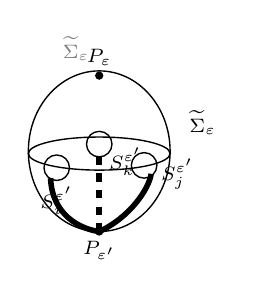
\begin{tikzpicture}[x=.6cm,y=.6cm,every node/.style={font=\scriptsize},line width=.5pt]
\draw (0,0) ellipse (1.5 and 1.7);
\draw (0,-.05) ellipse (1.5 and .35);
\draw (-.9,-.35) circle (.27); \draw (0,.15) circle (.27); \draw (.95,-.3) circle (.27);
\draw[line width=2pt] (-1.03,-.57) .. controls (-1,-1.35) and (-.4,-1.65) .. (0,-1.7) .. controls (.65,-1.4) and (1.05,-.8) .. (1.1,-.48);
\draw[line width=2pt,dashed] (0,-.12)--(0,-1.7);
\fill (0,1.6) circle (1.5pt); \fill (0,-1.7) circle (1.5pt);
\node[above] at (0,1.6) {$P_\varepsilon$}; \node[above left,gray] at (0,1.7) {$\widetilde\Sigma_\varepsilon$};
\node[below] at (0,-1.7) {$P_{\varepsilon'}$};
\node[right] at (0,-.22) {$S_k^{\varepsilon'}$}; \node[below] at (-.9,-.55) {$S_i^{\varepsilon'}$}; \node[right] at (1.1,-.48) {$S_j^{\varepsilon'}$};
\node[right] at (1.7,.6) {$\widetilde\Sigma_\varepsilon$};
\end{tikzpicture}
}
\[
(27)\quad\left\{\begin{aligned}
\widetilde\Sigma_\varepsilon&=\widetilde\Sigma\setminus\bigcup_{i\in J}\operatorname{supp}d_i^\varepsilon \qquad\varepsilon\in\uline{\varepsilon}\\
\widetilde\Sigma_i&=\widetilde\Sigma\setminus\bigcup_{\substack{j\in J\setminus\{i\}\\\deleted{\omega\in\uline{\omega}}}}\deleted{\operatorname{supp}}\unsure{b_i|b_j}^{\deleted{\unsure{\omega}}}
\end{aligned}\right.
\]
\margin{(où $b_i=\operatorname{supp}\widetilde b_i^\omega$\newline
\deleted{$=\operatorname{supp}\unsure{c_i^\omega|b_i^\omega}\cup\operatorname{supp}\unsure{c_i^{\omega'}|b_i^{\omega'}}$}\newline
$=\operatorname{supp}\unsure{c_i^\omega|b_i^\omega}\cup\operatorname{supp}\unsure{c_i^{\omega'}|b_i^{\omega'}}$)}
\figure{
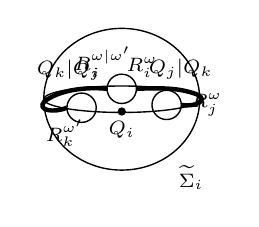
\begin{tikzpicture}[x=.6cm,y=.6cm,every node/.style={font=\scriptsize},line width=.5pt]
\draw (0,0) ellipse (1.65 and 1.5);
\draw (0,0) ellipse (1.65 and .28);
\draw (-.85,-.18) circle (.31); \draw (0,.22) circle (.31); \draw (.95,-.12) circle (.31);
\draw[line width=1.6pt] (-.31,.22) .. controls (-.8,.27) and (-1.35,.18) .. (-1.64,-.05) .. controls (-1.8,-.23) and (-1.45,-.3) .. (-1.16,-.18);
\draw[line width=1.6pt] (.31,.22) .. controls (.8,.24) and (1.2,.25) .. (1.6,.1) .. controls (1.85,-.03) and (1.55,-.17) .. (1.26,-.12);
\fill (0,-.26) circle (1.5pt); \node[below] at (0,-.26) {$Q_i$};
\node[above] at (-1.12,.2) {$\unsure{Q_k|Q_j}$}; \node[above] at (1.25,.22) {$\unsure{Q_j|Q_k}$};
\node[above] at (-.4,.25) {$R_i^{\unsure{\omega|\omega'}}$}; \node[above] at (.43,.25) {$R_i^\omega$};
\node[below] at (-1.2,-.22) {$\unsure{R_k^{\omega'}}$}; \node[right] at (1.26,-.12) {$R_j^\omega$};
\node[below right] at (1,-1.2) {$\widetilde\Sigma_i$};
\end{tikzpicture}
}
Ce sont bien des ouverts \deleted{\unsure{de }$\Sigma$} simplement connexes de la sphère à trous $\widetilde\Sigma$ (car les complémentaires \inserted{connexes et à} sont connexes. On dit que $P_\omega$ est le \uline{centre} de $\widetilde\Sigma_\omega$, $Q_i$ le \uline{centre} de $\widetilde\Sigma_i$.
\margin{ce sont des ouverts denses, et pour cette raison connexes.}
On pose
\[
(28)\quad\left\{\begin{aligned}
\Pi_\varepsilon&=\Pi_1(\widetilde\Sigma,\widetilde\Sigma_\varepsilon)\simeq\Pi_1(\Sigma^*,\Sigma_\varepsilon^*)\simeq\Pi_1(\Sigma^*,P_\varepsilon)\\
\Pi_i&=\Pi_1(\widetilde\Sigma,\widetilde\Sigma_i)=\Pi_1(\Sigma^*,\Sigma_i^*)\simeq\Pi_1(\Sigma^*,Q_i)
\end{aligned}\right.
\]
en faisant les identifications indiquées par ces formules. \deleted{\unsure{De}} Pour $\forall\ x\in\widetilde\Sigma_\omega$ resp. $x\in\widetilde\Sigma_i$, on pose
\[
(29)\quad\left\{\begin{aligned}
\varphi_{\varepsilon,x}\text{ ou }\varphi_\omega&:\Pi_\varepsilon\xrightarrow{\sim}\Pi_1(\widetilde\Sigma,x)\quad(\simeq\Pi_1(\Sigma^*,x)\text{ si }x\in\Sigma^*)\\
\varphi_{i,x}\text{ ou }\varphi_i&:\Pi_i\xrightarrow{\sim}\Pi_1(\widetilde\Sigma,x)\qquad\text{--}
\end{aligned}\right.
\]
\margin{Les $\varphi$ sont appelés \uline{isom.} \uline{de} \uuline{\unsure{transition|trivialisation}}.}
\margin{51}

\scanpage{53}
\mspage{6}
L'isom. canonique déduit de l'inclusion.

On a de plus des isomorphismes canoniques
\[
(30)\quad\left\{\begin{aligned}
\varphi_{i\varepsilon}&:\Pi_\omega\longrightarrow\Pi_i\qquad\text{défini par }c_i^\varepsilon:P_\varepsilon\longrightarrow Q_i\\
\varphi_{\varepsilon i}&:\Pi_i\longrightarrow\Pi_\omega\qquad\text{---}\qquad(c_i^\varepsilon)^{-1}:Q_i\longrightarrow P_\varepsilon
\end{aligned}\right.
\]
\margin{\uline{NB} on a $\varphi_{i\varepsilon}=\varphi_{Q_i,\varepsilon}$, $\varphi_{\varepsilon i}=\varphi_{P_\varepsilon,i}$.}
Par ces isom., les $\Pi_\varepsilon,\Pi_i$ sont reliés de façon transitive, mais bien entendu pas par un syst. transitif d'isomorphismes -- au contraire, les autom. d'un des groupes $\Pi_\varepsilon,\Pi_i$ obtenus en composant des isoms 30, suivant des chemins fermés sur le graphe
\figure{
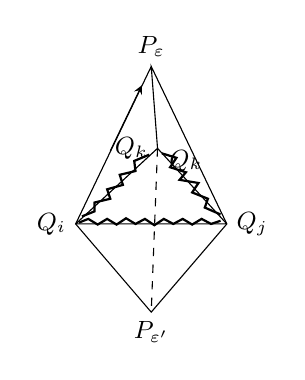
\begin{tikzpicture}[x=.8cm,y=.8cm,>=stealth,every node/.style={font=\small}]
\coordinate (P) at (0,2.5);\coordinate (M) at (0,-1.4);\coordinate (I) at (-1.2,0);\coordinate (J) at (1.2,0);\coordinate (K) at (.1,1.2);
\draw (P)--(I)--(M)--(J)--(P)--(K);
\draw[dashed] (K)--(M);
\draw[->] (-.65,1.16)--(-.15,2.2);
\draw (I)--(J) (I)--(K)--(J);
\draw[thick] (-1.15,.02)--(-1,.08)--(-.85,-.01)--(-.7,.08)--(-.55,-.01)--(-.4,.09)--(-.25,0)--(-.1,.08)--(.05,-.02)--(.2,.08)--(.35,0)--(.5,.08)--(.65,-.01)--(.8,.08)--(.95,0)--(1.1,.05);
\draw[thick] (-1.1,.12)--(-.9,.2)--(-.9,.34)--(-.65,.4)--(-.7,.55)--(-.45,.62)--(-.5,.78)--(-.25,.84)--(-.27,1)--(-.03,1.1);
\draw[thick] (.17,1.12)--(.4,1.05)--(.3,.9)--(.55,.82)--(.45,.7)--(.75,.65)--(.65,.5)--(.9,.4)--(.85,.26)--(1.1,.15);
\node[above] at (P) {$P_\varepsilon$};\node[below] at (M) {$P_{\varepsilon'}$};\node[left] at (I) {$Q_i$};\node[right] at (J) {$Q_j$};\node[left] at (K) {$Q_k$};
\node at (.55,1) {$\deleted{\unsure{Q_k}}$};
\end{tikzpicture}
}
sont \uline{tous} les autom. intérieurs !

Les $\Pi_1(\Sigma^*,\text{en }-)$ en les $P_\varepsilon,Q_i$ étant \unsure{canonifiés|canonisés} comme les $\Pi_\varepsilon,\Pi_i$, il reste à ``repérer'' les $\Pi_1$ en les autres sommets marqués jusqu'à maintenant. Les choix naturels sont par
\deleted{$\unsure{\varphi_\varepsilon}\ \Pi_\varepsilon\quad\unsure{\varphi_i}\ \Pi_i\longrightarrow$}
\margin{52}

\scanpage{54}
\[
(31)\quad\left\{\begin{aligned}
\varphi_{R_i^\omega,\omega i}&:\Pi_{\omega i}\xrightarrow{\sim}\Pi_1(\widetilde\Sigma,R_i^\omega)\\
&\text{ou }\varphi_{\omega i}\\
&\text{ou }c_{\omega i}^{\omega'}\\
\varphi_{S_i^\varepsilon,\unsure{\omega|\varepsilon}}&:\Pi_\omega\xrightarrow{\sim}\Pi_1(\widetilde\Sigma,S_i^\varepsilon)\\
&\text{ou }\varphi_\omega\\
&\text{ou }d_i^{\unsure{\varepsilon|\omega}}
\end{aligned}\right.
\]
Le plus commode me semble de noter simplement $\varphi_i,\varphi_\varepsilon$ pour préciser les groupes $\Pi_1$ \unsure{standart|standards} $\Pi_i$ ou $\Pi_\varepsilon$ qui sont des sources, le point base $a$ ($=R_i^\varepsilon$ ou $S_i^\varepsilon$, disons) ne faisant pas de doute dans le calcul.
\deleted{Les arcs $a_i^\omega$ sont :}
\deleted{Les arcs $a_i^\omega$ sont visiblement trop longs, il faut les couper en deux en posant
\[
(31)\quad\left\{\begin{aligned}
a_i^\omega&=a_i^{\omega-}a_i^{\omega+}\\
a_i^{\omega+}&:R_i^\omega\longrightarrow S_i^\omega\qquad a_i^{\omega-}:S_i^\omega\longrightarrow R_i^{\omega'}
\end{aligned}\right.
\]
}
Il faut enfin, pour des calculs formels, donner une façon de repérer les $\Pi_i,\Pi_\omega$ par un $=$ groupe \unsure{standart|standard} $\unsure{\Pi_{0,3}}$, pour lequel nous prendrons
\[
\begin{aligned}
(32)\qquad\Pi_{0,3}&=\Pi_1\left(\deleted{\unsure{\Sigma}}\overbrace{\mathbb P^1_{\mathbb C}\setminus\{0,1,\infty\}}^{U_{0,3}(\mathbb C)},P^+\right)\\
&=\{l_0,l_1,l_\infty\mid l_\infty l_1l_0=1\}\\
&\subset\widetilde\Pi_{03}=\Pi_1(U_{03}(\mathbb C),\mathcal G_3^*,\inserted{\times\{1,\tau\}}P^+)
\end{aligned}
\]
\[
=\{\rho,\sigma_\infty,\widetilde\sigma_\infty\mid \rho^3=\sigma_\infty^2\inserted{=\widetilde\sigma_\infty^2}=1,\quad \widetilde\sigma_\infty(\rho)=\rho^{-1},\quad\unsure{\widetilde\sigma_\infty(\widetilde\sigma_\infty)=1|\widetilde\sigma_\infty(\sigma_\infty)=1}\}
\]
\inserted{i.e. $(\sigma_\infty\widetilde\sigma_\infty)^2=1$}
\deleted{$=\{\rho,\sigma_\infty\mid\rho^3=\sigma_\infty^2=1\}\simeq\operatorname{SL}(2,\mathbb Z)/\{\pm1\}$}
\inserted{$\simeq\operatorname{GL}(2,\mathbb Z)/\{\pm1\}$}
\margin{53}

\scanpage{55}
\mspage{7}
avec le \unsure{formulaire géométrique|formulaire de génération} dans $\widetilde\Pi_{0,3}\simeq\unsure{\operatorname{SL}(2,\mathbb Z)|\operatorname{GL}(2,\mathbb Z)}$ :
\[
(33)\quad\left\{\begin{aligned}
\varepsilon_0&\overset{\mathrm{def}}=\sigma_\infty\rho\\
\varepsilon_1&\overset{\mathrm{def}}=\rho(\varepsilon_0)\quad(=\rho\varepsilon_0\rho^{-1})\\
\varepsilon_\infty&\overset{\mathrm{def}}=\rho(\varepsilon_1)=\rho^2(\varepsilon_0)=\rho^{-1}(\varepsilon_0)
\end{aligned}\right.
\qquad
\begin{aligned}
l_0&\overset{\mathrm{def}}=\varepsilon_0^2\\
l_1&\overset{\mathrm{def}}=\varepsilon_1^2\\
l_\infty&\overset{\mathrm{def}}=\varepsilon_\infty^2
\end{aligned}
\]
\[
l_\infty l_1l_0=1
\]
\margin{
$\rho(l_i)=l_{\rho(i)}\quad\left\{\begin{aligned}\rho(l_0)&=l_1\\\rho(l_1)&=l_\infty\\\rho(l_\infty)&=l_0\end{aligned}\right.$\newline
$\rho(\unsure{\varepsilon_i|l_i'})=\varepsilon_{\rho(i)}$\newline
\uline{NB} on fait opérer $\rho$ sur $0,1,\infty$ par $0\mapsto1\mapsto\infty\mapsto0$
}
\[
(33)\quad\left\{\begin{aligned}
\tau_\infty&\overset{\mathrm{def}}=\sigma_\infty\widetilde\sigma_\infty\unsure{=|,}\widetilde\sigma_\infty\sigma_\infty\\
\tau_\infty^2&=1
\end{aligned}\right.
\]
\[
\begin{aligned}
\tau_\infty(l_0)&=l_0^{-1}\\
\tau_\infty(l_1)&=l_1^{-1}\\
\tau_\infty(l_\infty)&=\unsure{l_0|l_0^{-1}}l_1=\unsure{\operatorname{int}(l_0)}(l_\infty^{-1})
\end{aligned}
\qquad
\begin{aligned}
\widetilde\sigma_\infty(l_0)&=l_1^{-1}\\
\widetilde\sigma_\infty(l_1)&=l_0^{-1}\\
\widetilde\sigma_\infty(l_\infty)&=l_\infty^{-1}
\end{aligned}
\]
\[
\begin{aligned}
\sigma_\infty(l_0)&=l_1\\
\sigma_\infty(l_1)&=l_0\\
\sigma_\infty(l_\infty)&=l_1^{-1}l_0^{-1}=\unsure{\operatorname{int}(l_0)}(l_\infty)
\end{aligned}
\]
Notons qu'un épinglage de la situation est donné par un élément du produit
\[
\operatorname{Rep}(J,\uline{\unsure{\bar\omega|\varpi}})\simeq J\times\uline{\omega}\times\uline{\unsure{\bar\omega|\varpi}}
\]
donc par la donnée d'un $(i,\omega,\unsure{\bar\omega|\varpi})$, définissant \deleted{donc} un $\varepsilon=\omega\wedge\unsure{\bar\omega|\varpi}\in\uline{\varepsilon}\simeq\uline{\omega}\wedge\uline{\unsure{\bar\omega|\varpi}}$. On va définir pour
\[
r=(i,\omega,\unsure{\bar\omega|\varpi})
\]
des isoms
\[
\deleted{\unsure{\Pi_{03}}}\qquad(34)\quad\left\{\begin{aligned}
\psi_{\deleted{\unsure{i}}\varepsilon}^{\deleted{\unsure{\omega}}i,\omega}&:\Pi_{03}\xrightarrow{\sim}\Pi_\varepsilon\\
\psi_{i\deleted{\unsure{\omega}}}^{\omega,\varepsilon}&:\Pi_{03}\xrightarrow{\sim}\Pi_i
\end{aligned}\right.
\]
\margin{isoms dits \uline{d'épinglage}}
donnant lieu comme de juste au triangle commutatif
\diagram{
\begin{tikzcd}[ampersand replacement=\&]
\& \Pi_{03}\arrow[dl,"\psi_{\deleted{\unsure{i}}\varepsilon}^{\deleted{\unsure{\omega}}i,\omega}"']\arrow[dr,"\psi_{i\deleted{\unsure{\omega}}}^{\omega,\varepsilon}"] \& \\
(35)\quad\Pi_\varepsilon\arrow[rr,shift left=.6ex,"\varphi_{i\varepsilon}","\sim"'] \& \& \Pi_i\arrow[ll,shift left=.6ex,"\varphi_{\varepsilon i}","\sim"']
\end{tikzcd}
}
\margin{54}

\scanpage{56}
ce qui fait qu'il suffit de définir l'un des deux isom. (34) -- et en vertu de la définition de $\Pi_{03}$ en (32), il est naturel de définir plutôt l'iso
\[
\deleted{(\unsure{35})}\qquad\psi_r=\psi_{\deleted{\unsure{\omega}}\varepsilon}^{i,\omega}:\Pi_{03}\xrightarrow{\sim}\Pi_\varepsilon
\]
\margin{$r=(i,\omega,\deleted{\unsure{\varepsilon}}\inserted{\unsure{\bar\omega|\varpi}})$}
par transport des structures comme
\[
(36)\quad\left\{\begin{aligned}
\psi_{\varepsilon\deleted{\unsure{\omega}}}^{i,\omega}&=\deleted{\Pi_1(\unsure{u_\varepsilon^{i,\omega}})}\Pi_1(u_{i,\omega,\varepsilon};P^+)\\
\text{où }\inserted{u_r=u_{i,\omega,\varepsilon}}\ u_\varepsilon^{i,\omega}&:(U_{0,3}(\mathbb C),P_+)\longrightarrow(\Sigma^*,P_\omega)
\end{aligned}\right.
\]
est l'unique iso conforme qui transforme le repère \deleted{\unsure{base}} standart \inserted{$(\infty,\omega_{0,1,\infty},+1)$} \deleted{\unsure{analogue}} dans le repère \deleted{$\unsure{(\omega i,\omega'i,i)}$} $(i,\omega,\varepsilon)$
\margin{Au couple $(i,\omega)$ on associe le repère (au sens habituel) $r=(\omega i,\omega'i,i)$ de $J$, i.e. \deleted{\unsure{correspondant}}
\[
0\longmapsto\omega i,\quad 1\longmapsto\omega^2i=\omega'i,\quad\infty\longmapsto i.
\]
Ainsi, on a, si $r=\deleted{\unsure{(\omega i,\omega'i,i)}}(i,\omega)$,
\[
\rho_\omega(r)=r\circ\rho=(\omega i,\omega).
\]
}
Pour un $P_\omega$ fixé, il y a six choix pour les \inserted{$\psi_r=$} $\psi_{\varepsilon\deleted{\unsure{\omega}}}^{i,\omega}:\Pi_{03}\longrightarrow\Pi_\varepsilon$ -- et pour un $Q_i$ fixé, il y a quatre choix pour $\omega,\varepsilon$. Cela fait \inserted{trois resp.} deux choix si on suppose que l'on a choisi une \unsure{valeur} de $\unsure{\bar\omega|\varpi}$ sur $\Sigma$ et réalisé \unsure{donc} $\uline{\varepsilon}\simeq\uline{\omega}$, et si on se borne aux $\varepsilon$ qui correspondent à $\omega\ \unsure{\Rightarrow}$ -- il faut donc voir comment passer de l'un \inserted{de ces choix} à l'autre.
\margin{55}

\scanpage{57}
\mspage{9}
Notons que l'isom
\[
\psi_r:\Pi_{03}\xrightarrow{\sim}\Pi_\omega
\]
\inserted{$r\in\operatorname{Rep}(J,\uline{\unsure{\bar\omega|\varpi}})\ \deleted{\unsure{pour}}\simeq\operatorname{Isom}((\Sigma_0^*,P_+),(\Sigma^*,P_+))$}
est compatible avec le transport des structures, \deleted{ce qui fait} donc pour $\forall$ élément
\[
g\in\widetilde{\mathcal G}_J\subset\Gamma=\mathcal G_J
\]
\inserted{
\[
\begin{aligned}
\widetilde{\mathcal G}_J=\Gamma_{P_\varepsilon}&=\left\{(g,\tau^{\unsure{\operatorname{sg}g|\alpha}})\in\mathcal G_J\times\deleted{\{1,\tau\}}\inserted{\mathbb Z/2\mathbb Z}\ \middle|\ \begin{array}{l}\alpha=0\text{ si }\operatorname{sg}g=1\\\alpha=1\text{ si }\operatorname{sg}g=-1\end{array}\right\}\\
&=\{g\in\Gamma\mid \unsure{g_\varepsilon^{(\varepsilon)}|g(\varepsilon)}=\operatorname{id}_{\unsure{\varepsilon}}\}
\end{aligned}
\]
}
on aura commutativité de
\diagram{
\begin{tikzcd}[ampersand replacement=\&]
\&\Pi_{03}\arrow[dl,"\psi_r=\psi_{\omega,i}^\varepsilon"']\arrow[dr,"\psi_{g(r)}=\psi_{g(\omega),g(i)}^{g(\varepsilon)}"]\&\\
(37)\quad\Pi_\varepsilon\arrow[rr,"\Pi_1(g)","\text{(par transport de structure)}"']\&\&\Pi_\varepsilon
\end{tikzcd}
}
ce qui suffit en principe à passer d'un $\psi_r$ à $\psi_{g(r)}=\deleted{\unsure{\varphi}}\Pi_1(g)\circ\psi_r$, vu que \deleted{\unsure{g}} $\widetilde{\mathcal G}_J$ est simplement transitif sur l'ens. des repères $r$ correspondant à un $\varepsilon$ fixé. Mais, on aimerait exprimer le passage par une formule de transformation \uline{dans} $\Pi_{0,3}$.

Notons que la donnée du repère \inserted{$r$} définit un isom canonique (encore noté $u_r$)
\margin{56}

\scanpage{58}
\[
u_r:\widetilde{\mathcal G}_3\xrightarrow{\sim}\widetilde{\mathcal G}_J
\]
et tout repère $r'$ \inserted{\unsure{au $=$ $\varepsilon$ près|avec $=$ $\varepsilon$ pour $r$}} sera de la forme de façon unique
\[
r'=rg_0\quad\text{avec }g_0\in\widetilde{\mathcal G}_3
\]
\[
(38)\quad\text{i.e.}\quad u_{r'}=u_ru_{g_0}\qquad(\text{avec }u_r(g_0)=g\text{ mais peu importe})
\]
d'où, en passant à l'action sur les $\Pi_1$ en $P_+$ resp. $P_\varepsilon$, on trouve
\[
(39)\qquad \psi_{r'\deleted{\unsure{\varepsilon}}}=\psi_r\circ\Pi_1(g_0,P_+)\qquad\text{si }r'=r\circ g_0.
\]
\margin{$\psi_r,\psi_{r'}$ désignent ici les isom\unsure{s}. d'épin\unsure{g}lage associés \deleted{aux} à $P_\varepsilon$.}
On va expliciter ceci pour
\[
g_0=\rho\quad\text{donc }r'=r\rho=(\omega i,\omega,\unsure{\bar\omega|\varpi})\quad\text{si }r=(i,\omega,\unsure{\bar\omega|\varpi})
\]
On trouve
\[
\psi_\varepsilon^{\omega i,\omega}=\inserted{\rho_\omega\circ\psi_\varepsilon^{i,\omega}=}\psi_\varepsilon^{i,\omega}\circ\rho
\]
où on a identifié $\rho$ aussi à un élément de $\widetilde\Pi_{0,3}$, et à l'autom qu'il induit sur $\Pi_{0,3}$.

\uline{NB} $\rho_\omega$ est la rotation autour de $P_\varepsilon,P_{\varepsilon'}$ d'un tiers de tour, \deleted{\unsure{suivant}} l'orientation $\omega$ sur l'équateur.

\margin{\uline{NB}\quad $\psi_\varepsilon^{i,\omega}(l_0),\psi_\varepsilon^{i,\omega}(l_1),\deleted{\unsure{\psi_\varepsilon^{i,\omega}(l_0)}}$ sont resp. les lacets \unsure{tournant|fondés} à partir de $P_\varepsilon$, autour des trous $R_{\omega i},R_{\unsure{\omega^2}i}$, \deleted{\unsure{qui}} passant $Q_i$ (donc \unsure{au détriment de} $\unsure{R_i|R_{\omega\prime i}}$ : \unsure{$R_{\omega i}\cdots$}), et dans le sens d'orientation $\unsure{\bar\omega|\varpi}=\omega\wedge\varepsilon$.}
\figure{
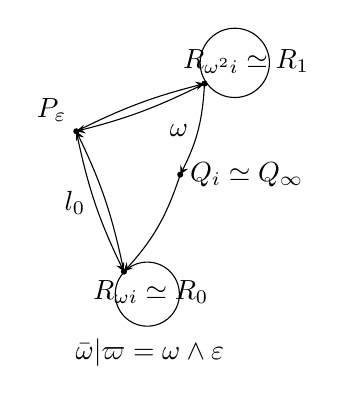
\begin{tikzpicture}[scale=1.1,>=stealth]
\coordinate (p) at (0,1);\coordinate (q) at (1.2,0.5);\coordinate (r0) at (.55,-.62);\coordinate (r1) at (1.48,1.55);
\fill (p) circle(1pt) node[above left]{$P_\varepsilon$};
\fill (q) circle(1pt) node[right]{$Q_i\simeq Q_\infty$};
\fill (r0) circle(1pt);\fill (r1) circle(1pt);
\draw (0.82,-0.88) circle (0.37);\draw (1.83,1.79) circle(0.4);
\node at(0.86,-0.86){$R_{\omega i}\simeq R_0$};\node at(1.96,1.81){$R_{\omega^2i}\simeq R_1$};
\draw[->] (p) to[bend right=7] node[left]{$l_0$} (r0);
\draw[->] (r0) to[bend right=7] (p);
\draw[->] (p) to[bend left=6] (r1);\draw[->] (r1) to[bend left=6] (p);
\draw[<-] (r0) to[bend right=12] (q);\draw[<-] (q) to[bend right=12] node[left]{$\omega$} (r1);
\node[below]at(0.85,-1.28){$\unsure{\bar\omega|\varpi}=\omega\wedge\varepsilon$};
\end{tikzpicture}}
On trouve de $=$, pour un autom qui renverse l'orientation de $\sigma$, i.e. pour un
\[
\widetilde\sigma_\infty:\quad\begin{array}{rcl}0&\longrightarrow&1\\1&\longrightarrow&0\\\infty&\longrightarrow&\infty\end{array}\qquad\deleted{\unsure{la}}\unsure{\bar\omega|\varpi}\longmapsto\unsure{\bar\omega|\varpi}'
\]
\deleted{$\unsure{\widetilde\sigma_\infty}$}
\[
g_0=\widetilde\sigma_\infty\qquad r'=r\widetilde\sigma_\infty=(\deleted{\unsure{\omega}}i,\omega',\unsure{\bar\omega|\varpi}').
\]
d'où
\[
(41)\qquad\psi_\varepsilon^{\deleted{\unsure{\omega}}i,\omega'}=\inserted{\widetilde\sigma_i\circ\psi_\varepsilon^{i,\omega}=}\psi_\varepsilon^{i,\omega}\circ\widetilde\sigma_\infty
\]
($\widetilde\sigma_i$ est la symétrie p.r. \unsure{au|du} grand cercle méridien passant par $Q_i$)
\margin{57}

\scanpage{59}
\mspage{10}
Passons au cas de $Q_i$ -- la définition \unsure{évidente} \deleted{\unsure{géométrique}} des
\[
\psi_r=\psi_i^{\omega,\varepsilon}:\quad\Pi_{0,3}-\Pi_i\deleted{(\unsure{Q_i})}
\]
est
\[
\inserted{\psi_r=}\psi_i^{\omega,\varepsilon}=\Pi_1(\underbrace{u_{i,\omega,\varepsilon}}_{u_r};Q_\infty)
\]
\margin{\uline{NB} on identifie la \inserted{source $\Pi_1(U_{0,3};Q_\infty)$} \deleted{\unsure{source}} à $\Pi_{03}\stackrel{\mathrm{def}}=\Pi_1(U_{0,3};P_+)$ à l'aide du chemin standard $d_\infty^+$ de $P_+$ à $Q_\infty$.}
\unsure{Donc} $u_r=u_{i,\omega,\varepsilon}$ est l'unique isom de $U_{0,3}$, \inserted{dans $\Sigma^*$} qui transforme le repère \deleted{fixé} standard $(\infty,\omega_0=+1,\unsure{\bar\omega|\varpi}_0=+1\text{ donc }\varepsilon=\omega_0\wedge\unsure{\bar\omega|\varpi}_0=+1)$ en $r$ i.e. qui transforme $P_+$ en $P_\varepsilon$, $Q_0$ en $Q_i$, $Q_1$ en $Q_{\omega i}$. \deleted{On} Les épinglages \deleted{\unsure{par un repère fixé}} de $\Pi_i$ \inserted{$\psi_i^{\omega,\varepsilon}$ ($i$ fixé, $\omega,\varepsilon$ variables)} correspondent aux $u_r$ qui transforment $Q_0$ en $Q_i$, ils sont donc déterminés par composition avec des éléments
\[
g_0\in\Gamma_0=\mathcal G_3\times\{1,\tau\}
\]
qui stabilisent $Q_0$ -- ces éléments \deleted{engendrent} font un groupe $\simeq\mathbb Z/2\times\mathbb Z/2$ engendré par $\sigma_\infty,\tau$, \deleted{et} On trouve encore
\[
\psi_{r'}^{\deleted{\unsure{\omega}}}=\psi_r\circ\deleted{\unsure{\psi}}\Pi_1(g_0;Q_\infty)\quad\text{si }r'=r\circ g_0
\]
où ici $\psi_{r'},\psi_r$ désignent les iso. d'épinglage relatifs à $Q_i$. Il suffit d'expliciter ces formules dans les cas de $g_0=\sigma_\infty,g_0=\tau$, ce qui revient à calculer leur effet sur $\deleted{\unsure{\Pi_{0,3}=}}\Pi_1\deleted{\unsure{\varepsilon}}(U_{0,3};\unsure{Q_\infty|R_\infty})$, quand on identifie celui-ci à $\Pi_{03}=\Pi_1(U_{0,3};P_+)$, grâce au chemin $d_\infty^+$ de $P_+$ à $Q_\infty$. On sait que l'on peut
\margin{58}

\scanpage{60}
$\operatorname{int}(\sigma_\infty),\operatorname{int}(\tau_\infty)$,
\inserted{Or dans ce cas $g_0=\tau_\infty$ resp. $g_0=\sigma_\infty$, \deleted{\unsure{donc}} \inserted{on} trouve $r'=(i,\omega,\varepsilon')$ resp. $r'=(i,\omega',\varepsilon')$, donc}
\[
(39)\qquad\begin{cases}
\psi_i^{\omega,\varepsilon'}=\tau\circ\psi_i^{\omega,\varepsilon}=\psi_i^{\omega,\varepsilon}\circ\tau_\infty\\[5pt]
\psi_i^{\omega',\varepsilon'}=\underbrace{\sigma_i}_{\substack{\text{transposition}\\\in\mathcal G_J\text{ qui}\\\text{fixe }i}}\circ\psi_i^{\omega,\varepsilon}=\psi_i^{\omega,\varepsilon}\circ\sigma_\infty
\end{cases}
\]
donc en composant
\[
(40)\qquad\psi_i^{\omega',\varepsilon\deleted{\unsure{'}}}=\deleted{\unsure{\tau}}\underbrace{\widetilde\sigma_i}_{\substack{\tau\sigma_i\\\text{symétrie}\\\text{autour du}\\\text{grand cercle}\\\text{passant par}\\P_\varepsilon,P_{\varepsilon'},Q_i}}\circ\psi_i^{\omega,\varepsilon}=\psi_i^{\omega,\varepsilon}\circ\widetilde\sigma_\infty
\]
Dans tous ces calculs, suivant sans doute d'anciennes habitudes, j'ai privilégié les $P_\varepsilon$ et les $Q_i$ comme p\textsuperscript{ts} base -- alors que pour le travail que j'ai à faire, ce sont les points $R_i^\omega$ qui sont les plus cruciaux, où les calculs faits en ces p\textsuperscript{ts} capturent directement les phénomènes de ``monodromie'' autour des ``trous'' $R_i$. Je vais réparer cette négligence, en introduisant, en
\margin{59}

\scanpage{61}
plus des $\deleted{\widetilde\Pi_\omega}\Pi_\omega$ et $\deleted{\widetilde\Pi_i},\Pi_i$, des régions
\[
\widetilde\Sigma_r=\widetilde\Sigma_{\deleted{\unsure{r}}i\deleted{\unsure{\omega}}}^{\omega,\varepsilon}
\]
associés aux repères $r=(i,\omega,\deleted{\unsure{\bar\omega|\varpi}}\varepsilon)$ de $(J,\uline{\varepsilon})$ (ou ce qui revient au $=$, de $(J,\uline{\unsure{\bar\omega|\varpi}})$), qu'on peut identifier, géométriquement, aux \inserted{douze} triangles-drapeaux, \inserted{$D_r=P_\varepsilon Q_iR_{\omega i}$} correspondants à la subdivision barycentrique standard de la carte dans $\Sigma$ définie par l'équateur $\Sigma_{\mathbb R}$ et par les trois points $R_i$ sur celui-ci.
\figure{
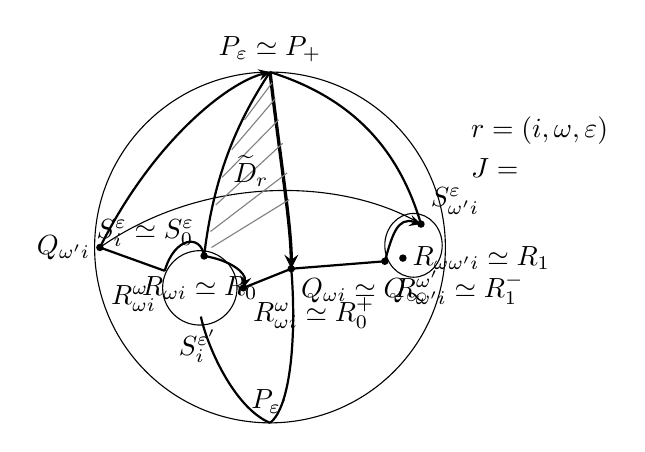
\begin{tikzpicture}[scale=1.35,>=stealth]
\coordinate (N) at(0,1.65);\coordinate (S)at(0,-1.65);\coordinate (L)at(-1.6,0);\coordinate (Q)at(.2,-.2);\coordinate (T)at(1.25,-.1);\coordinate (A)at(-.62,-.08);\coordinate (B)at(-.25,-.38);\coordinate (C)at(1.08,-.13);\coordinate (D)at(1.42,.22);
\draw[thin] (0,0)circle(1.65);
\draw[thin] (L) .. controls(-.6,.7)and(.7,.65)..(D);
\draw[->,thick] (L)..controls(-1.1,1.0)and(-.4,1.55)..(N);
\draw[thick] (N)..controls(.8,1.4)and(1.22,.9)..(D);
\draw[thick] (N)..controls(-.4,1.05)and(-.55,.5)..(A);
\draw[->,very thick] (N)..controls(.1,.8)and(.2,.2)..(Q);
\draw[thick] (Q)..controls(.25,-.8)and(.2,-1.5)..(S);
\draw[thick] (S)..controls(-.35,-1.5)and(-.6,-.9)..(-.65,-.65);
\draw[thick] (L)--(-.99,-.22);\draw[thick] (B)--(Q)--(C);
\draw[->,thick] (-.99,-.22)..controls(-.9,.1)and(-.65,.13)..(A)..controls(-.37,-.12)and(-.22,-.24)..(B);
\draw[thin] (-.66,-.38)circle(.35);
\draw[->,thick] (C)..controls(1.15,.12)and(1.2,.29)..(D);
\draw[thin] (1.35,.02)ellipse(.27 and .3);
\foreach \a/\b/\c/\d in {-.56/.15/.16/.7,-.51/.4/.12/.98,-.45/.66/.08/1.2,-.36/.92/.05/1.4,-.24/1.2/.02/1.55,-.55/.0/.18/.45}{\draw[thin,gray](\a,\b)--(\c,\d);}
\node at(-.18,.72){$\widetilde D_r$};
\node[above] at(N){$P_\varepsilon\simeq P_+$};\node[above]at(S){$P_{\varepsilon'}$};
\node[left]at(L){$Q_{\omega'i}$};\node[below right]at(Q){$Q_{\deleted{\unsure{\omega}}i}\simeq Q_\infty$};
\node[above left]at(A){$S_i^\varepsilon\simeq S_0^\varepsilon$};\node[below]at(-.68,-.68){$S_i^{\varepsilon'}$};
\node[below left]at(-.98,-.2){$R_{\unsure{\omega i}}^{\omega'}$};
\node[below right]at(B){$R_{\unsure{\omega i}}^\omega\simeq R_0^+$};
\node at(-.66,-.38){$R_{\deleted{\unsure{\omega}}i}\simeq\deleted{\unsure{R_0}}$};
\node[below right]at(C){$R_{\omega'i}^{\omega'}\simeq R_1^-$};
\node[above right]at(D){$S_{\omega'i}^\varepsilon$};
\node[right]at(T){$R_{\deleted{\unsure{\omega}}\omega'i}\simeq R_1$};
\node[right]at(1.8,1.1){$r=(i,\omega,\varepsilon)$};\node[right]at(1.8,.75){$J=$};
\fill(L)circle(1pt);\fill(Q)circle(1pt);\fill(A)circle(1pt);\fill(B)circle(1pt);\fill(C)circle(1pt);\fill(D)circle(1pt);\fill(T)circle(1pt);
\end{tikzpicture}}
Le ``\unsure{tronc|vrai}'' \inserted{sur $\widetilde\Sigma$} au sens évident d'un tel triangle est un quadrilatère $\widetilde D_r$
\[
P_\varepsilon Q_{\omega'i}R_i^\omega S_i^\varepsilon\simeq P_+Q_\infty R_0^+S_0^+.
\]
On aura à travailler, au ``voisinage'' immédiat de ces \deleted{repères} \inserted{drapeaux} \deleted{\unsure{triangles des}} $\widetilde\Sigma_r$, avec les symétriques de $\Sigma_r$ p.r. à ses trois côtés, et \unsure{se trouve sur|par suite sur} $\widetilde\Sigma$, \deleted{\unsure{pour ce qui}} ce qui conduit à regarder la réunion de $\Sigma_r$ avec ses trois frères
\[
\tau(\Sigma_r),\widetilde\sigma_i(\Sigma_r),\widetilde\sigma_{\omega i}(\Sigma_r)
\]
(qui \inserted{resp.} correspondent, sur la sphère standard avec le repère correspondant au triangle $P_+Q_\infty R_0$, à $\tau,\widetilde\sigma_\infty,\widetilde\sigma_0$) et sur $\widetilde\Sigma$ à prendre
\[
(41)\qquad\widetilde\Sigma_r=\widetilde\Sigma_i^{\omega,\varepsilon}=\widetilde D_r\cup\tau(\widetilde D_r)\cup\widetilde\sigma_i(\widetilde D_r)\cup\widetilde\sigma_{\omega i}(\unsure{\Sigma_+|\Sigma_r})
\]
limités par le contour
\[
P_\varepsilon Q_{\omega'i}R_{\omega i}^{\omega'}S_i^{\unsure{\varepsilon|\varepsilon'}}R_{\omega i}^{\omega}S_i^{\varepsilon'}P_{\varepsilon'}Q_iR_{\omega'i}^{\omega'}S_{\omega'i}^\varepsilon P_\varepsilon
\]
\margin{60}

\scanpage{62}
correspondant, sur la sphère standard, à la région ci-contre, délimitée par le contour
\[
P_+Q_1R_0^-\unsure{S_0^+|D_0^+}R_0^+S_0^-P_-Q_\infty R_1^-S_1^+P_+
\]
\figure{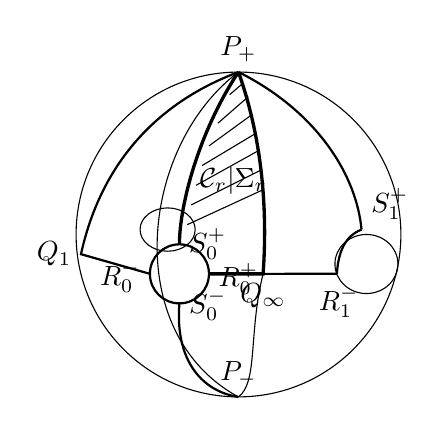
\begin{tikzpicture}[scale=1.25,>=stealth]
\coordinate(N)at(0,1.65);\coordinate(S)at(0,-1.65);\coordinate(L)at(-1.6,-.2);\coordinate(Q)at(.25,-.4);
\draw[thin](0,0)circle(1.65);
\draw[thin](N)..controls(-1,.9)and(-1.2,-1)..(S);
\draw[thick](N)..controls(-1.2,1.2)and(-1.5,.25)..(L)--(-.9,-.4);
\draw[very thick](N)..controls(-.4,1.05)and(-.6,.3)..(-.6,-.1);
\draw[very thick](N)..controls(.23,1)and(.3,.3)..(Q)--(-.3,-.4);
\draw[thick](Q)--(1,-.4);\draw[thick](N)..controls(.8,1.25)and(1.2,.6)..(1.25,.05);
\draw[thick](-.6,-.4)circle(.3);\draw[thin](1.3,-.3)ellipse(.32 and .3);
\draw[thick](1,-.4)..controls(1.02,-.05)and(1.18,.02)..(1.25,.05);
\draw[thin](-.72,.05)ellipse(.28 and .22);
\draw[thick](-.6,-.7)..controls(-.65,-1.3)and(-.35,-1.6)..(S);
\draw[thin](Q)..controls(.1,-1)and(.2,-1.5)..(S);
\foreach \a/\b/\c/\d in {-.52/.1/.24/.45,-.48/.3/.22/.65,-.43/.5/.2/.85,-.37/.7/.18/1.03,-.3/.9/.14/1.22,-.21/1.13/.1/1.4,-.09/1.42/.05/1.54}{\draw[thin](\a,\b)--(\c,\d);}
\node[above]at(N){$P_+$};\node[above]at(S){$P_-$};\node[left]at(L){$Q_1$};\node[below]at(Q){$Q_\infty$};
\node[left]at(-.9,-.43){$R_0^-$};\node[right]at(-.3,-.45){$R_0^+$};\node[right]at(-.6,-.1){$S_0^+$};\node[right]at(-.6,-.72){$S_0^-$};
\node[below]at(1.02,-.43){$R_1^-$};\node[above right]at(1.25,.05){$S_1^+$};
\node at(-.05,.55){$\unsure{\mathcal C_r|\Sigma_r}$};
\end{tikzpicture}}
Les régions $\widetilde\Sigma_r$ sont permutées de façon simplement transitive par $\Gamma=\mathcal G_J\times(1,\tau)$. Elles sont simplement connexes, et permettent donc de définir des
\[
\deleted{(42)}\qquad\Pi_r=\Pi_i^{\omega\varepsilon}=\Pi_1(\widetilde\Sigma;\widetilde\Sigma_r)=\Pi_1(\Sigma^*;\Sigma_r^*)
\]
\deleted{et des isom} \deleted{qui} mais qui sont reliés par un syst. transitif d'iso. à l'aide du gr. de $\Gamma$, de sorte qu'on peut identifier tous ces groupes entre eux. En fait, on trouve des isom. d'épinglage
\[
(42)\qquad\Psi_r:\Pi_{0,3}\longrightarrow\Pi_r=\unsure{\Pi_i|\Pi}^{\omega,\unsure{i|\varepsilon}}=\Pi_1(\widetilde\Sigma;\widetilde\Sigma_r)
\]
($\psi_r$ majuscule

\deleted{en identifiant}
en composant
\diagram{\begin{tikzcd}[ampersand replacement=\&,column sep=large]
\Pi_{03}\arrow[r,shorten >=1.7em]\arrow[r,"\psi_r=\psi_\varepsilon^{\omega,i}"]\&\begin{array}{c}\Pi_1(\widetilde\Sigma,P_\varepsilon)\\\simeq\Pi_1(\Sigma^*,P_\varepsilon)\end{array}\arrow[r,leftrightarrow,"\varphi_r^{-1}"]\&\Pi_r
\end{tikzcd}}
où \deleted{$\unsure{\varphi}$}
\[
\varphi_r:\Pi_r\longrightarrow\Pi_\varepsilon=\Pi_1(\widetilde\Sigma,P_\varepsilon)
\]
est l'``isomorphisme de transition'' correspondant à la région $1$-connexe $\Sigma_r$, et au point $P_\varepsilon$ de $\Sigma_r$.
\margin{61}

\scanpage{63}
\mspage{12}
La donnée d'un $R_i^\omega$, \inserted{qu'on va écrire $R_{\omega i}^{\omega}$, équivaut à} celle d'un repère \inserted{$r=(i,\omega)$} de $J$, et définit \uline{deux} \deleted{\unsure{rég}} régions $\widetilde D_r$ qui le contiennent, correspondant aux deux repères de $(J,\unsure{\uline{\varepsilon}|\varepsilon})$ qui prolongent $r$ -- et il y a donc deux régions correspondantes $\widetilde\Sigma_r$, qui sont les seules qui contiennent $R_i^\omega$ comme \uline{point intérieur} (NB. dans la région $\widetilde\Sigma_{r_0}$ standard, les deux autres points $R$ à part $R_0^+$, qui est intérieur, sont $R_0^-$ et $R_1^-$, qui ne le sont pas). Mais si la sphère $\Sigma$ est orientée i.e. si on s'est donné un élément marqué \inserted{$\unsure{\bar\omega|\varpi}_+$} de $\uline{\unsure{\bar\omega|\varpi}}=\uline{\omega}\wedge\uline{\varepsilon}$, ou encore un isom $\varepsilon\simeq\uline{\varepsilon}$, alors le point $R_i^\omega$ détermine un $\varepsilon$ \inserted{$\in\uline{\varepsilon}$} privilégié, par la condition que $\varepsilon$ corresponde à $\omega$ par $\uline{\omega}\simeq\uline{\varepsilon}$ ou encore que $\omega\wedge\varepsilon=\unsure{\bar\omega|\varpi}_+$, ce qui signifie aussi que l'orientation $P_+S_0^+R_0^+Q_\infty P_+$ de la région $\deleted{\widetilde\Sigma_r}\widetilde D_r$ est \deleted{celle de} $\unsure{\bar\omega|\varpi}_+$. Donc on peut alors identifier canoniquement, via $\psi_r$, $\Pi_1(\widetilde\Sigma,R_i^\omega)$ à $\Pi_{0,3}$, par un iso (qui dépend du choix de l'orientation $\unsure{\bar\omega|\varpi}_+$ de $\Sigma$)
\[
(43),\qquad\psi_i^\omega:\Pi_{03}\xrightarrow{\sim}\Pi_1(\widetilde\Sigma,R_i^\omega)
\]
\margin{62}

\scanpage{64}
de sorte qu'on aura \deleted{compatibilité} \inserted{commutativité} de
\diagram{\begin{tikzcd}[ampersand replacement=\&,column sep=large,row sep=large]
\&\Pi_{03}\arrow[dl,"\unsure{\Psi|\psi}_i^\omega"',"\deleted{\Pi_{03}}"]\arrow[d,"\psi_i^{\omega\deleted{\unsure{\varepsilon}}}"]\arrow[dr,"\psi_\omega^i"]\&\\
(44)\quad\Pi_{\unsure{0|1}}(\widetilde\Sigma,R_{\omega i}^\omega)\&\begin{array}{c}\Pi_1(\widetilde\Sigma,Q_i)\\=\Pi_i\end{array}\arrow[l,"b_i^{\omega'}(\cdot)"',"{\deleted{\unsure{\rightarrow}}}"{description,pos=.08}]\&\begin{array}{c}\Pi_1(\widetilde\Sigma,P_\omega)\\=\Pi_\omega\end{array}\arrow[l,"\varphi_{i\omega}=c_i^\omega(\cdot)"',"{\deleted{\unsure{\rightarrow}}}"{description,pos=.08}]
\end{tikzcd}}
où on a écrit $P_\omega$ au lieu de $P_\varepsilon$ (en identifiant $\uline{\omega}$ et $\uline{\varepsilon}$ grâce à $\unsure{\bar\omega|\varpi}_+$) et $\psi_i^\omega$ au lieu de $\psi_i^{\omega,\omega}$, $\psi_\omega^i$ au lieu de $\psi_\omega^{i,\omega}$.

Le passage à expliciter est celui de
\diagram{\begin{tikzcd}[ampersand replacement=\&,column sep=large]
\deleted{R_{\omega i}}\Pi_i^\omega\simeq\Pi_1(\widetilde\Sigma,R_{\omega i}^{\omega})\&\text{à}\&\Pi_i^{\omega'}=\Pi_1(\widetilde\Sigma,R_{\omega'i}^{\omega'})\\
\Pi_{0,3}\arrow[u,"\psi_i^\omega","\sim"']\&\&\Pi_{03}\arrow[u,"\psi_i^{\omega'}","\sim"']
\end{tikzcd}}
\inserted{via $\widetilde b_{i\omega}$.}
\figure{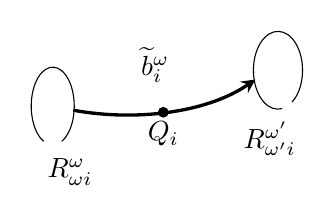
\begin{tikzpicture}[scale=1.3,>=stealth]
\draw(-.089,-.344)arc[start angle=245,end angle=-65,x radius=.21,y radius=.38];\draw(2.242,-.024)arc[start angle=280,end angle=-55,x radius=.24,y radius=.38];
\draw[->,very thick](.2,-.04)..controls(.8,-.15)and(1.5,-.07)..(1.98,.26);
\fill(1.08,-.06)circle(1.5pt)node[below]{$Q_i$};\node at(1,.4){$\widetilde b_i^\omega$};
\node[below]at(.17,-.42){$R_{\omega i}^{\omega}$};\node[below]at(2.12,-.06){$R_{\omega'i}^{\omega'}$};
\end{tikzpicture}}
On trouve par la commutativité (44) et par la dernière formule (39) qu'on a
\deleted{$\unsure{\widetilde b_{\omega\omega'}}$}
\[
(45)\qquad\widetilde b_i^\omega\bigl(\psi_i^\omega(\deleted{\unsure{g}}x)\bigr)=\psi_i^{\omega'}\bigl(\sigma_\infty(x)\bigr).
\]
\margin{63}

\scanpage{66}
\margin{(\unsure{38|39} pages)}
\mspage{\unsure{5}}
Généralités sur les actions du groupe de Galois sur les \unsure{compactifiés|complétés} profinis de groupoïdes fondamentaux de variétés Alg. complexes
\margin{65}

\scanpage{67}
\mspage{1}
Soit $K$ un sous-corps du corps des complexes $\mathbb C$ -- des cas intéressants seront celui où $K=\mathbb Q$, ou $K$ extension finie de $\mathbb Q$, ou $K=\widetilde{\mathbb Q}$ extension abélienne maximale de $\mathbb Q$ dans $\mathbb C$ -- je serai intéressé en tous cas avant tout aux cas où $K$ est de t.f. sur $\mathbb Q$. (Le cas de $\widetilde{\mathbb Q}$ est un cas ``limite'' de tels cas, pour ne pas être gêné par les racines de $1\ldots$).

On s'intéresse aux schémas \inserted{$X$} de t.f. sur $K$, et aux espaces \inserted{analytiques} $X(\mathbb C)$ correspondants. Comme on s'intéresse aux invariants ``topologiques'' de $X,X(\mathbb C)$, on traitera les morphismes $X'-X$ qui induisent des homéomorphismes universels comme des iso -- en particulier les éléments nilpotents ne comptent pas -- une imm. fermée surjective sera traitée comme un iso.

Un langage commode est de considérer $X$ comme donné par l'espace analytique (ou $=$ seulement topologique) $X(\mathbb C)$, plus une \uline{structure} supplémentaire dessus : la structure de ``var. alg. sur $K$'', à coups de top. de Zariski, de faisceau des fonctions $K$-polynomiales etc. On écrira par la suite $X$ au lieu de $X(\mathbb C)$.

On distingue sur $X$ le groupoïde fondamental $\Pi_1(X)$ au sens topologique, et son compactifié profini $\widehat\Pi_1(X)$, qui \deleted{\unsure{est en un sens}} \inserted{peut} aussi être défini directement en fonction du $\mathbb C$-schéma $X$. On a un foncteur ``d'inclusion''
\margin{66}

\scanpage{68}
\[
(1)\qquad\Pi_1(X)\unsure{\relbar\joinrel\relbar|\longrightarrow}\widehat\Pi_1(X)
\]
qui induit une bijection sur l'ens des objets \inserted{ou ``sommets''} -- s'identifiant à $X=X(\mathbb C)$ -- et qui \deleted{déf} pour $\forall x\in X=X(\mathbb C)$, donne l'hom de groupes
\[
(2)\qquad
\begin{array}{ccc}
\operatorname{Aut}_{\Pi_1(X)}(x)&\longrightarrow&\operatorname{Aut}_{\widehat\Pi_1(X)}(x)\\
\Vert\ \text{déf}&&\Vert\ \text{déf}\\
\pi_1(X,x)&&\widehat\pi_1(X_{\mathrm{sch}},x)
\end{array}
\]
permettant d'identifier le $\pi_1$ algébrique au compactifié profini du $\pi_1$ ``topologique'' ou ``transcendant'' : \unsure{b}
\[
(3)\qquad\pi_1(X_{\mathrm{sch}},x)\simeq\widehat\pi_1(X,x).
\]
De $=$, pour $x,y\in X$, l'application
\[
\operatorname{Hom}_{\Pi_1(X)}(x,y)\longrightarrow\operatorname{Hom}_{\widehat\Pi_1(X)\deleted{\unsure{y}}}(x,y)
\]
\margin{On identifiera un élément de $\operatorname{Hom}_{\Pi_1}(x,y)$ avec son image dans $\operatorname{Hom}_{\widehat\Pi_1}(x,y)$, sans se préoccuper si l'application est injective ou non.}
permet d'identifier le deuxième ens, en tant que bi-torseur sur $(\widehat\pi_1(X,y),\widehat\pi_1(X,x))$ au bitorseur déduit \deleted{Hom} du premier ens par extension des groupes d'opérateurs par
\[
\pi_1(X,y)\unsure{\relbar\joinrel\relbar|\longrightarrow}\widehat\pi_1(X,y),\qquad\pi_1(X,x)\unsure{\relbar\joinrel\relbar|\longrightarrow}\widehat\pi_1(X,x).
\]
(ce couple d'homomorphismes satisfaisant \inserted{bien} à la condition requise pour que cette extension ait un sens\ldots).
\margin{à savoir (en termes de $(G,H),(G',H')$ et $G\to G',H\to H'$ : il existe un isom ext. $G'\xrightarrow{\sim}H'$ rendant commutatif le diagramme \deleted{\unsure{des bitorseurs}}
\diagram{\begin{tikzcd}[ampersand replacement=\&,column sep=large,row sep=large]
G\arrow[r,"\sim", "\substack{\text{défini par le}\\\text{bitorseur }(G,H)}"']\arrow[d]\&H\arrow[d]\\
G'\arrow[r,"\sim"]\&H'
\end{tikzcd}}}
Soit
\[
(5)\qquad\unsure{\mathbf{\Gamma}|\Gamma}_{\deleted{K}}=\unsure{\mathbf{\Gamma}|\Gamma}_K=\operatorname{Aut}_{K\text{-cor}}(\mathbb C),
\]
\margin{67}

\scanpage{69}
\mspage{2}
alors $\unsure{\mathbf{\Gamma}|\Gamma}$ opère non seulement sur \deleted{$X$} l'ens. $X$, mais aussi sur le groupoïde $\widehat\Pi_1(X)$, à cause du fait que celui-ci admet une définition purement schématique, ne faisant pas intervenir la topologie de $\mathbb C$. Bien entendu, si $\lambda:\deleted{x} x\to y$ dans $\Pi_1$, alors pour $u\in\Gamma$, $u(\lambda)$ n'est \unsure{p|pas} en général une flèche de $\Pi_1$ (de $u(x)$ vers $u(y)$) mais seulement de $\widehat\Pi_1$.

\deleted{Notation} Notation ${}^ux$ ($x\in X,u\in\unsure{\mathbf{\Gamma}|\Gamma}$) et \deleted{\unsure{``}}
\[
{}^u\lambda:{}^ux-{}^uy\qquad\text{si }\lambda:x\to y\quad(\text{dans }\widehat\Pi_1(X)).
\]
On a
\[
(6)\qquad\begin{cases}
{}^u(\operatorname{id}_x)=\operatorname{id}_{{}^ux}\qquad(x\in X)\\
{}^u(\mu\lambda)={}^u\mu\,{}^u\lambda
\end{cases}
\]
\diagram{\(\left(\begin{tikzcd}[ampersand replacement=\&,column sep=large]
x\arrow[r,"\lambda"]\&y\arrow[r,"\mu"]\&z\\
{}^ux\arrow[r,"{}^u\lambda"]\&{}^uy\arrow[r,"{}^u\mu"]\&{}^uz
\end{tikzcd}\right)\)}
Notre objet est d'essayer de ``déterminer'' autant que faire se peut cette action de $\unsure{\mathbf{\Gamma}|\Gamma}$. À vrai dire, si $\bar K$ est la clôture algébrique de $K$ dans $\mathbb C$, on s'intéressera surtout aux sous-groupoïdes de $\Pi_1(X)$ et $\widehat\Pi_1(X)$ induits sur l'ens d'objets $X_{\bar K}$, qu'on désignera par $\Pi_1(X_{\bar K}),\widehat\Pi_1(X_{\bar K})$ -- le deuxième est stable par l'action de $\unsure{\mathbf{\Gamma}|\Gamma}$, et si on pose
\[
(7)\qquad\Gamma=\operatorname{Aut}_{K\text{-cor}}(\bar K)=\operatorname{Gal}_{\bar K/K},
\]
de sorte que $\Gamma$ est un quotient de $\unsure{\mathbf{\Gamma}|\Gamma}$, l'action de $\unsure{\mathbf{\Gamma}|\Gamma}$ sur $\Pi_1(X_{\bar K})$ se fait à travers $\Gamma$. $\uparrow$
\margin{68}

\scanpage{70}
Pour décrire l'action d'un $u\in\unsure{\mathbf{\Gamma}|\Gamma}$ (resp $u\in\Gamma$) sur $\widehat\Pi_1(X)$ (resp. $\widehat\Pi_1(X_{\bar K})$), on prendra comme ``générateurs'' du groupoïde $\widehat\Pi_1$ des chemins provenant de $\Pi_1$. On aura, pour ${l}:x\to y$ dans $\Pi_1$, ${}^u{l}:{}^ux\to{}^uy$.

Si \deleted{on suppose} par la suite, pour simplifier, on se borne à des points $x,y\ldots$ rationnels sur $\unsure{X|K}$ -- i.e. qu'on travaille dans le sous-groupoïde $\widehat\Pi_1(X_K)$ formé des objets qui sont invariants sous $\unsure{\mathbf{\Gamma}|\Gamma}$ -- alors on aura
\[
(*)\qquad{}^u{l}:{}^ux=x\longrightarrow{}^uy=y,
\]
et on peut écrire, \deleted{\unsure{f}}
\[
(8)\qquad\begin{cases}
{}^u{l}=g_{l}(u)\circ{l}={l}\circ f_{l}(u)\\
g_{l}(u)\in\widehat\pi_1(X,y)\\
f_{l}(u)\in\widehat\pi_1(X,x)
\end{cases}
\]
\deleted{$g_{l}(u)={}^u{l}\circ{l}^{-1}$}
\figure{\begin{tikzpicture}[x=2mm,y=2mm]
\node at(0,0){,};
\fill(.5,.8)circle(.07);\fill(.75,.55)circle(.07);\fill(1.25,.4)circle(.08);\fill(1.75,.08)circle(.045);
\fill[gray](1.16,-.08)circle(.04);\fill[gray](1.38,-.1)circle(.035);
\end{tikzpicture}}
\margin{On écrira aussi parfois $g_u({l})$ au lieu de $g_{l}(u)$, $f_u({l})$ pour $f_{l}(u)$.}
où $f_{l}(u),g_{l}(u),{}^u{l}$ se déterminent mutuellement, \deleted{\unsure{fonctoriquement}} par les formules (8) et
\[
(9)\qquad\begin{cases}
f_{l}(u)={l}^{-1}\cdot{}^u{l},\quad g_{l}(u)={}^u{l}\cdot{l}^{-1}\\
g_{l}(u)={l}(f_{l}(u)),\quad f_{l}(u)={l}^{-1}(g_{l}(u))
\end{cases}
\]
On décrira l'action d'un $u\in\Gamma$ \inserted{sur un sous-groupoïde plein de $\Pi_1(X)$} à l'aide des éléments $f_{l}(u)$, ou $g_{l}(u)$, pour un syst. de générateurs convenable des \inserted{groupoïdes pleins} correspondants de $\Pi_1(X)$. Dans le cas d'un
\margin{69}

\scanpage{71}
\mspage{3}
sous-groupoïde induit sur une partie \uline{\unsure{finie}} \deleted{\illegible{1}} $I$ de $X_K$, on pourra trouver un nb fini de tels générateurs --- il suffit p.ex. de choisir un \deleted{\unsure{$x$}} $x_0\in I$, et choisir pour tt $x\in I\setminus x_0$ un chemin $l_x$ de $x_0$ \unsure{à} $x$, et de plus un syst. \inserted{fini} de générateurs $l_i$ de $\Pi_1(X,x_0)$.

Il apparaît que sous des conditions assez générales (p.ex. si $X$ est une variété alg. \unsure{anabélienne}) la connaissance de l'opération $u$ sur $\widehat{\Pi}_1(X_K,I)$ (\inserted{pour un} $u\in\Gamma$) \uline{suffit à} déterminer $u$ --- et la question se pose alors de voir comment la connaissance des invariants \inserted{disons} $g_{l_\alpha}(u)$ (pour un syst. générateur de flèches $l_\alpha$ de $\Pi_1(X,\unsure{I})$) permet de retrouver les invariants $g_l(u)$ pour d'autres \inserted{$K$-}schémas $Y\ldots$.
\margin{\figure{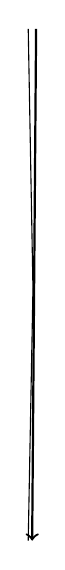
\begin{tikzpicture}[x=1mm,y=1mm]\draw (0,0)--(.6,32)--(0,65);\draw[->,line width=.8pt] (1,65)--(.5,0);\end{tikzpicture}}}

Quand il s'agit du $=$ schéma $X$, et qu'on s'intéresse \unsure{à} d'autres chemins $l:x\longrightarrow y$ $(x,y\in I)$ que les générateurs choisis $l_\alpha$, la formule donne en principe un moyen de reconstituer les $g_l(u)$ pour tout $l$, puisqu'il permet de retrouver les ${}^u l$, et que ${}^u l$ est multiplicatif en $l$. En termes des $g_l(u)$, \deleted{\unsure{$g_l(u)$}}, la formule de multiplicativité (6) s'écrit, pour une situation
\margin{\uline{NB} pour le moment, on ne regarde que les $x\in X_K$ qui sont dans $I$, le \unsure{syst} fini de \unsure{points} choisi.}
\diagram{\begin{tikzcd}[ampersand replacement=\&,column sep=large]
x\arrow[r,no head,"\unsure{l'|l}"] \& y\arrow[r,no head,"\unsure{l''|l'}"] \& z
\end{tikzcd}}
\[
(10)\qquad \unsure{g_{ll'}(\deleted{ll'}u)}=g_l(u)\cdot l\bigl(g_{l'}(u)\bigr)
\qquad\text{soit }g_u(ll')=g_u(l)\cdot l\bigl(g_u(l')\bigr)
\]
\margin{70}

\scanpage{72}
et en termes des $f\ldots$ la formule, est identique mais d'allure un peu moins \unsure{sympathique}
\[
(11)\qquad f_{ll'}(u)=l'^{-1}\bigl(f_l(u)\bigr)\cdot f_{l'}(u)
\qquad\text{i.e. }f_u(ll')=l'^{-1}f_u(l)\cdot f_u(l')
\]

\deleted{La formule (6) peut s'exprimer en disant que pour $l$ fixé, $u\in\Gamma$ variable,
\[
(12)\qquad g_l:\Gamma\longrightarrow\widehat{\Pi}_1(X,y)
\]
est un $1$-cocycle sur $\Gamma$, à valeurs dans $\widehat{\Pi}_1(X,y)$, relativement à l'action naturelle de $\Gamma$ sur $\widehat{\Pi}_1(X,y)$. Bien entendu, le $\widehat{\Pi}_1(X,y)$-torseur à gauche, \inserted{sur qui opère $\Gamma$,} correspondant à ce $1$-cocycle, n'est autre que $\operatorname{Hom}_{\widehat{\Pi}_1(X)}(x,y)$, sur lequel $\widehat{\Pi}_1(X,y)=\operatorname{Hom}_{\widehat{\Pi}_1(X)}(y,y)$ opère par composition.}

Pour un composé d'une \deleted{\unsure{nb fini}} suite finie composable de chemins
\diagram{\begin{tikzcd}[ampersand replacement=\&]
x_0\arrow[r,"l_1"]\&x_1\arrow[r,"l_2"]\&\cdots\&x_{n-1}\arrow[r,"l_n"]\&x_n
\end{tikzcd}}
la formule (10) prend la forme
\[
\unsure{(13)|(12)}\qquad
 g_{l_nl_{n-1}\cdots l_1}(u)=g_{l_n}(u)\cdot l_n\bigl(g_{l_{n-1}}(u)\bigr)\cdot l_nl_{n-1}\bigl(g_{l_{\unsure{n-2}}}(u)\bigr)\ldots
 \inserted{\cdot(l_n\cdots l_2)g_{l_1}(u))}
\]
Formule la plus \deleted{évidente} \inserted{simple} possible en somme de celles qu'on pourrait imaginer qui ait un sens. On va \unsure{développer} \deleted{encore} \inserted{un} contexte qui permette \deleted{mieux} d'écrire cette formule, ainsi que \deleted{\unsure{(11)}} la formule analogue en $f$ et les formules
\margin{71}

\scanpage{73}
\mspage{4}
(9) de passage de $f$ à $g$, sous une forme considérablement plus simple.

Soit $T$ un espace topologique \deleted{simplement} $1$-connexe, et
\[
(13)\qquad p:T\longrightarrow X
\]
une application continue \inserted{(le cas \unsure{injectif} sera le plus intéressant)}. Soit $T_K=p^{-1}(X_K)$.

Considérons \deleted{\unsure{$\Pi_1(T_K),\ \Pi_1$}}
\deleted{\unsure{Soient} $x,y\in T_K$}
\[
\unsure{(14)}\qquad\deleted{\unsure{\Pi_1(X)}}\ \Pi_1(X;T)=\pi
\]
alors pour tout $x\in T$ on a un isom canonique
\[
(15)\qquad\varphi_x:\pi\xrightarrow{\sim}\Pi_1(X,p(x))
\]
\inserted{de sorte que les $\Pi_1(X,p(x))$ sont munis d'un syst. transitif d'iso}
\margin{On désigne \unsure{ainsi|aussi} par $\varphi_x$ le prolongement aux complétés profinis\ldots}
et pour $x,y\in T$, l'unique \deleted{élément} \inserted{flèche} \deleted{de Hom} $x:y$ de $\Pi_1(T)$ donne \inserted{par $p$} une flèche canonique
\[
\unsure{(16)}\qquad l_{y,x}:p(x)\mathbin{-}p(y)\qquad\text{dans }\Pi_1(X)
\]
(NB cette flèche dépend du choix de $x,y$ au dessus de $px,py$ --- mais naturellement $p$ sera injective).

Moyennant les iso (15), on peut considérer $f_{l_{y,x}}(u)$ et $g_{l_{y,x}}(u)$ (\inserted{du moins} si $x,y\in T_K$ i.e. $p(x),p(y)\in X_K$) comme des éléments du $=$ groupe $\pi$ \unsure{(14)}, \deleted{soit} et en fait ces deux éléments se réduisent à un seul et $=$ élément, soit
\[
\begin{array}{c}
\unsure{(17)}\qquad g_{y,x}^{T/X}(u)=g_{y,x}^{p}(u)=\varphi_y^{-1}\bigl(g_{l_{y,x}}(u)\bigr)=\varphi_x^{-1}\bigl(f_{l_{y,x}}(u)\bigr)\\
\rotatebox{90}{$\in$}\\
\pi=\Pi_1(X;T)
\end{array}
\]
\margin{72}

\scanpage{74}
Les formules (10) (11) se réduisent donc à la formule
\[
(18)\qquad g_{zy}(u)g_{yx}(u)=g_{zx}(u)\qquad x,y,z\in T_K
\]
\margin{On a laissé tomber l'exposant $T$ : $g_{yx}^{T/X}$, qui est \unsure{nécessaire} surtout si $T\subset X\ldots$}
et la formule (12) à la formule itérée de celle-ci
\[
(19)\qquad g_{x_n,x_0}=g_{x_n,x_{n-1}}\,g_{x_{n-1},x_{\unsure{n-2}}}\cdots g_{x_1,x_0}
\]
--- quant aux formules de passage (9), elles \deleted{\unsure{tombent}} disparaissent !

Bien entendu, les invariants $g_l(u)$ \inserted{ou $f_l(u)$} peuvent être considérés comme décrits par des invariants précédents du type $g_{y,x}^T$, en prenant \deleted{\unsure{$T$}} p.ex. $T=[0,1]$, $p$ une application $[0,1]\longrightarrow X$ \unsure{donnant} naissance \deleted{au} chemin $l$ (plutôt, à la classe de chemins\ldots) de sorte qu'on aura
\[
(20)\qquad f_l(u)=\varphi_x\bigl(g_{y_0,x_0}^T(u)\bigr),\qquad g_l(u)=\varphi_y\bigl(g_{y_0,x_0}^T(u)\bigr)
\]
\deleted{$x_0=0\in T,\ y_0$}
\[
x_0=0,\ \deleted{\unsure{0}}\ y_0=1\qquad\in T=[0,1].
\]
\margin{Autre exemple ``\unsure{illuminant}'' : si $x_0\in X_K$ fixé, pour les $y\in X_K$ ``voisins'' de $\unsure{X|x_0}$, \unsure{choisissons} des chemins ``directs'' $x_0\longrightarrow y$ (``voisins'' de $x_0$) on trouve des invariants $g_{y,x_0}(u)\in\Pi_1(X,x_0)$.}

\deleted{La relation de $1$-cocycle}
\deleted{Bien entendu,}
\deleted{On peut}
Pour comparer les invariants $g_{x,y}^T$ associés à différents espaces $1$-connexes au dessus de $X$, il suffit de regarder le cas où on a un diag. comm.
\diagram{\begin{tikzcd}[ampersand replacement=\&,column sep=large]
T\arrow[rr,"f"]\arrow[dr,"p"'] \&\& T'\arrow[dl,"p'"]\\
\&X\&
\end{tikzcd}}
\[
(21)
\]
d'où $f_K:T_K\mathbin{-}T'_K$,
\margin{73}

\scanpage{75}
\mspage{5}
et un homomorphisme
\[
(22)\qquad\pi=\Pi_1(X;T/X)\overset{\psi=\Pi_1(f)}{\unsure{\mathbin{-}|\longrightarrow}}\pi'=\Pi_1(X,T'/X)
\]
Ceci dit, si $x,y\in T_K$, d'où $x'=f(x),y'=f(y)\in T'_K$, on aura
\[
(23)\qquad g_{y',x'}^{T'}(u)=\psi\bigl(g_{y,x}^T(u)\bigr)
\qquad(x'=f(x),y'=f(y),\psi=\Pi_1(f))
\]

Conséquence pratique : Supposons $X=\bigcup_{\alpha\in A}T_\alpha$, les $T_\alpha$ $1$-connexes, d'où des \deleted{fonctions} \inserted{groupes}
\[
\deleted{\unsure{g_\alpha|f_\alpha}:\unsure{\Gamma\times}T_{iK}\times T_{iK}\longrightarrow}
\]
\[
(24)\qquad \pi_\alpha\overset{\text{déf}}{=}\Pi_1(X,T_\alpha)
\]
et des fonctions
\[
(25)\qquad\left\{\begin{aligned}
T_{\alpha K}\times T_{\alpha K}\times\Gamma&\longrightarrow\unsure{\pi_i|\pi_\alpha}\\
(x,y,u)&\longmapsto g_{y,x}^{T_\alpha}(u)\overset{\text{déf}}{=}g_{y,x}^{\alpha}(u)
\end{aligned}\right.
\]
satisfaisant la formule de multiplicativité (19).

Pour relier les fonctions entre elles, \deleted{il faut} on \deleted{\unsure{considère les groupes}} \inserted{sait que pour} $T_\alpha\subset T_\beta$, on a
\[
(26)\qquad\deleted{\unsure{\forall}}\ \varphi_{\beta\alpha}:\pi_\beta\mathbin{-}\pi_\alpha
\]
et les relations
\[
(27)\qquad\deleted{g}\quad g_{y,x}^{\beta}(u)=\varphi_{\beta\alpha}\bigl(g_{y,x}^{\alpha}(u)\bigr)\qquad\begin{gathered}x,y\in T_{\alpha K}\\u\in\Gamma\end{gathered}
\]
Supposons que l'ens d'indices $\unsure{\mathbb{I}|I}$, avec sa relation d'ordre induite par l'inclusion $T_\alpha\subset T_\beta$, soit tel que \deleted{$\Pi_0(I)\unsure{\leftrightarrow|\longrightarrow}\Pi_0(X)$ est bijectif}
\[
(28)\qquad\forall\alpha,\beta\in I,\quad\text{on a}\quad T_\alpha\cap T_\beta=\bigcup_{\gamma\le\alpha,\beta}T_\gamma
\]
\[
\deleted{\Pi_0(I)\xrightarrow{\sim}\Pi_0(X)}
\]
\margin{74}

\scanpage{76}
\deleted{(\unsure{enfin} la surjectivité est \unsure{acquise}) que $T_\alpha,T_\beta$ sont dans une $=$ comp. connexe de $X$, il existe une ``chaîne'' d'\uline{indices}
\[
i_0=i,\ i_1,\ldots,i_n=j
\]
telle que pour deux indices consécutifs $k=i_r$, $k'=i_{r+1}$, on ait $T_k\subset T_{k'}$ ou $T_{k'}\subset T_k$.}
\margin{Supposons de plus que les intérieurs des $T_\alpha$ recouvrent $X$ ou que les $T_\alpha$ soient fermés (\deleted{et} $A$ fini) Alors on a $\Pi_0(A)\xrightarrow{\sim}\Pi_0(X)$. Mieux ---}

Supposons de plus \inserted{que les intérieurs des $T_i$ recouvrent $X$,} \deleted{\unsure{que $T_i$ est}} \inserted{\uline{Ceci posé,}} je dis que la connaissance des (pour $u$ fixé) des $g_{y,x}^\alpha(u)\in\pi_\alpha$ \inserted{($\alpha\in A,y,x\in T_\alpha$)} permet de retrouver \unsure{tous} les invariants $g_l(u)$ (ou $f_l(u)$). En effet, il suffit de voir que les flèches $l_{y,x}^\alpha=p_\alpha(l_{y,x})$ ($\alpha\in I$, $x,y\in T_\alpha$, $p_\alpha:T_\alpha\hookrightarrow X$ l'inclusion) \deleted{\unsure{eng}} forment un syst. de générateurs du groupoïde $\Pi_1(X_K)$\deleted{\unsure{$x_0$}} --- \inserted{tous} les \deleted{obj} sommets sont obtenus en tous cas, et on trouve une application bijective sur les $\Pi_0$ (du groupoïde engendré par les gén. $l_{y,x}^\alpha$ \inserted{($\alpha\in I,x,y\in T_{\alpha K}$) et les relations $l_{y,x}^{\unsure{\alpha|\beta}}=\varphi_{\beta\alpha}(l_{y,x}^{\alpha})$} et de $\Pi_1(X_K)$), il faut voir qu'on a une application surjective sur les $\Pi_1$.

Quand les intérieurs des $T_{\unsure{\alpha}}$ recouvrent $X$, il suffit de noter que la connaissance des $g_{y,x}^{\alpha}(u)$ nous donne les $g_{y,x}(u)$ (sans exposant $\alpha$ !) pour $x,y$ points ``voisins'' sur $X$,
\margin{75}

\scanpage{77}
\mspage{6}
or tout chemin effectif $x\longrightarrow y$ (donné par une appl continue $[0,1]\longrightarrow X$) se décompose en \inserted{composé de} chemins \inserted{``directs''}
\diagram{\begin{tikzcd}[ampersand replacement=\&,column sep=small]
x_0=x \arrow[r,no head] \& x_1 \arrow[r] \& x_2 \cdots \arrow[r,no head] \& x_n=y
\end{tikzcd}}
entre \deleted{\unsure{chemins|chemin}} \inserted{points} ``proches''. Dans le cas \deleted{général}, \inserted{où les $X_\alpha$ sont fermés} un argument de descente (comme déjà signalé dans la première hypothèse) donne le résultat énoncé.

Cette deuxième démonstration a l'avantage de marcher également pour \inserted{montrer} le résultat un peu plus général, et peut-être plus intéressant du point de vue pratique, où pour $\unsure{\forall|\text{tt}}\alpha$ on a $I_\alpha\subset T_\alpha$ partie \inserted{non vide} de $T_\alpha$ (normalement, partie finie) de telle façon que pour $T_\alpha\subset T_\beta$ on ait $I_\alpha\subset I_\beta$ (normalement, on prend d'abord $I\subset X_K$ convenable et on prend $I_\alpha=I\cap T_\alpha$, donc $I=\bigcup I_\alpha$), et on se borne aux $g^\alpha_{y,x}$ pour $x,y\in I_\alpha$: leur connaissance permet de retrouver \uline{tous} \inserted{$f_l(u)$,} $g_{\deleted{\unsure{yx}}l}(u)$, $l$ un chemin quelconque dans

\margin{On a deux façons de ``récupérer'' l'opération de $\Gamma$ sur le groupoïde $\widehat{\Pi}_1(X,I)$ (où $I\subset X_K$) en quelque sorte duales l'une de l'autre: soit on prend \unsure{un syst.} de $l_j:x_j\mathbin{-}y_j$ $(x_j,y_j\in I)$ générateurs pour $\Pi_1(X,I)$, et regarde les $f_{l_j}(u)$ ou $g_{l_j}(u)$, soit on fixe des $T_\alpha$ comme dessus, et on regarde les $g^\alpha_{x,y}$ $(\alpha\in A,x,y\in T_\alpha\cap I)$. En fait on voit que \unsure{très|trop} \unsure{bientôt} qu'il est \deleted{\unsure{ff}} inutile de supposer que les $T_\alpha$ \unsure{recouvrent|recouvrir} $X$ (p.ex. si les $T_\alpha$ sont les supports des chemins \unsure{$l_j$}).}

\figure{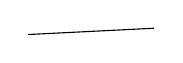
\begin{tikzpicture}\draw (0,0)--(1.6,.08);\end{tikzpicture}}
Jusqu'à présent, on a maintenu $u$ fixe, on a fait varier $l$, resp. $(T/X,x,y)$. Si on regarde ce qui se passe pour $u\in\Gamma$ variable, les formules
\margin{76}

\scanpage{78}
\unsure{essentielle triviale|essentielles triviales}, qui fait penser à (6), est
\[
\tag{28}{}^{uv}l={}^u({}^vl)
\qquad u,v\in\Gamma,\quad l:x\longrightarrow y\quad\text{chemin dans }\widehat\Pi_1(X),
\]
\deleted{d'où,} si $l$ est chemin de $\Pi_1(X)$, d'où
\[
{}^vl=g_l(v)\cdot l
\]
\deleted{\unsure{qui est alors}} d'où on tire par (6)
\[
{}^u({}^vl)={}^u\{g_l(v)\}\cdot\underbrace{{}^ul}_{g_l(u)\cdot l}
={}^ug_l(v)g_l(u)\cdot l
\]
d'où on tire
\[
\tag{29}\left\{\begin{aligned}
\deleted{\unsure{u}}g_l(uv)&={}^ug_l(v)\cdot g_l(u)\qquad\text{soit}\\
g_l^{-1}(uv)&=g_l^{-1}(u)\cdot{}^ug_l^{-1}(v)
\end{aligned}\right.
\]
\unsure{Et de $=$}
\[
\tag{30}f_l(uv)=f_l(u)\cdot{}^uf_l(v)
\]
i.e. $\unsure{f_l|f_{l\alpha}}$ et $g_l^{-1}$ sont, pour $l$ fixé, $\unsure{u|\text{en}}$ variable, des $1$-cocycles \inserted{sur $\Gamma$} à valeurs dans $\widehat\Pi_1(X,x)$ resp. $\widehat\Pi_1(X,y)$, \inserted{(groupes sur lesquels $\Gamma$ opère)}, d'ailleurs déduits l'un de l'autre par l'isomorphisme
\diagram{\begin{tikzcd}[ampersand replacement=\&]
\widehat\Pi_1(X,x)\arrow[r,no head,"\Pi_1(l)"]\&\widehat\Pi_1(X,y)
\end{tikzcd}}
induit par $l$ \deleted{\unsure{en $l$}}. Ici, c'est la formule pour $f_l$ qui a une gueule plus sympathique que celle pour $g_l$ (pour (10)(11) c'était l'inverse --- \inserted{exprim.} ``multiplicativité en $l$''). Les $1$-cocycles obtenus (\deleted{et} \inserted{$f$ un $1$-cocycle} droit, $g$ un $1$-cocycle à gauche) correspondent à des $\Gamma$ torseurs à droite resp. à gauche sous $\widehat\Pi_1(X,x)$ resp! $\widehat\Pi_1(X,y)$, qui bien sûr n'est autre que $\operatorname{Hom}_{\widehat\Pi_1(X)}(x,y)$

\margin{On pourrait \unsure{exploiter|expliciter} \unsure{un de vue qui voit le|au demeurant le} couple $(f_l,g_l)$ comme un ``bicocycle'' sur $\Gamma$, relatif à un $\Gamma$-bitorseur $\operatorname{Hom}_{\widehat\Pi_1(X)}(x,y)$ sous $(\widehat\Pi_1(X,y),\widehat\Pi_1(X,x))$.}
\margin{77}

\scanpage{79}
\mspage{7}
dont $l$ est justement un élément prenant le rôle d'un ``élément origine'', pour en déduire des $1$-cocycles\ldots

\deleted{Le théorème de Mordell-Weil implique que si $K$ est un corps de type fini sur $Q$, et si $X$ peut se plonger dans une \inserted{VA, ou dans un} groupe algébrique ext. d'une \uline{VA par un tore,} \uline{alors pour $x_0$ fixé,}}

Si on garde $x,y$, et qu'on remplace $l$ par un $l':x\longrightarrow y$, alors \deleted{\unsure{on}} on aura
\[
l'=la=bl\qquad a\in\Pi_1(X,x),\ b\in\Pi_1(X,y)
\]
et on aura, en vertu de (10)(11)
\[
\tag{31}\left\{\begin{aligned}
f_{l'}(u)&=\operatorname{int}(a^{-1})f_l(u)\underbrace{f_a(u)}_{a^{-1}\cdot{}^ua}=a^{-1}\cdot f_l(u)\cdot{}^ua\\
g_{l'}(u)&=\underbrace{g_b(u)}_{{}^ub\cdot b^{-1}}\operatorname{int}(b)\underbrace{g_l(u)}_{\deleted{\unsure{a^{-1}\cdot{}^ua}}}={}^ub\,g_l(u)b^{-1}
\end{aligned}\right.
\]
\[
(\text{i.e. }g_{l'}^{-1}(u)=b\,g_l^{-1}(u)\,{}^ub^{-1})
\]
\unsure{enfin}, $f_{l'}$ est un $1$-cocycle \inserted{à droite} homologue à $f_l$, $g_{l'}$ un $1$-cocycle \unsure{à g.} homologue à $g_l$. Ainsi, pour $x,y\in X_K$, on trouve des éléments
\[
\tag{32}\left\{\begin{aligned}
g_{y,x}&\in H^1_{\unsure{g}}(\Gamma,\widehat\Pi_1(X,y))\\
f_{y,x}&\in H^1_{\mathrm{dr}}(\Gamma,\widehat\Pi_1(X,x))
\end{aligned}\right.
\]
\deleted{\unsure{donc}} qui sont ``associés'' en un sens convenable, via les isom extérieurs canoniques
\diagram{\begin{tikzcd}[ampersand replacement=\&]
\widehat\Pi_1(X,x)\arrow[r,"\substack{\mathrm{isom}\\\mathrm{ext}}","\sim"']\&\widehat\Pi_1(\unsure{Y|X},y)
\end{tikzcd}}

\margin{Les $f_l(u),g_l(u)$ sont définis, et les formules \unsure{déjà de type|de type} (31) valables, sans \unsure{qu'on exige que} $l:x\longrightarrow y$ provienne de $\Pi_1(X)$, seulement de $\widehat\Pi_1(X)$. Et la définition des classes de $f_{\unsure{y}},g_{\unsure{y}}$ (ou classes de cohomologie) (32) ne dépend pas des (32) considérations transcendantes, ni de la \unsure{fixation du} corps de base $\mathbb C$\ldots}
\margin{78}

\scanpage{80}
toute la structure étant décrite canoniquement en termes du bitorseur $\operatorname{Hom}_{\widehat\Pi_1(X)}(x,y)$ sous $(\widehat\Pi_1(X,y),\widehat\Pi_1(X,x))$ et l'opération de $\Gamma$ sur \deleted{tout} ce fourbis. On se rappellera surtout que $f_{\unsure{y,x}}$ et $g_{y,x}$ se déterminent mutuellement, et qu'ils sont déterminés par la connaissance d'\uline{un seul} \deleted{$f_l$ \inserted{$:\Gamma\mathbin{-}\widehat\Pi_1(X,x)$} \unsure{(ou}} \deleted{$g_l$ (i.e. $f_l(u)$)} $f_l$, ou $g_l$
\[
\tag{33}\left\{\begin{aligned}
f_l&:\Gamma\unsure{\mathbin{-}|\longrightarrow}\widehat\Pi_1(X,x)\\
g_l&:\Gamma\unsure{\mathbin{-}|\longrightarrow}\widehat\Pi_1(\unsure{Y|X},y)
\end{aligned}\right.
\qquad l:x\mathbin{-}y\quad(\text{dans }\Pi_1(X))
\]
(Si on a \deleted{\unsure{un}} un $T^\alpha$ $1$-connexe $\subset X$, contenant $x,y$) ils sont connus quand on connaît seulement $g^{T^\alpha}_{x,y}$.

\margin{\uline{NB} $f_{x,y}$ et $f_{y,x}$, ou $g_{x,y}$ et $g_{y,x}$, se déterminent mutuellement, car, en termes du chemin $l$, on a
\[
\tag{34}\left\{\begin{aligned}
g_{l^{-1}}(u)&=f_l(u)^{-1}\\
f_{l^{-1}}(u)&=g_l(u)^{-1}
\end{aligned}\right.
\]}

Quand $X$ se plonge dans une VA, plus généralement s'il se plonge dans une extension d'une VA par un tore (p.ex. $X$ courbe alg. ``\unsure{anabélienne|abélienne}''), alors le th. de Mordell-Weil implique que pour un $x_0$ \inserted{$\in X_K$} fixé (comme pt de référence --- mais ce $x_0$ \deleted{\unsure{vient}} joue un rôle bidon!)
\margin{79}

\scanpage{81}
\mspage{8}
un point $x\in X_K$ est entièrement déterminé par la connaissance de \deleted{$f_{x_0,x}$}
\[
f_{x_0,x}\in H^1_{\mathrm{dr}}(\Gamma,\widehat\Pi_1\underbrace{(X,x_0)}_{\widehat{\unsure{\pi|\Pi}}(x_0)}),
\]
et a fortiori par la connaissance du $1$-cocycle
\[
f_l:\Gamma\longrightarrow\widehat\Pi^{\unsure{\text{ét}}}(x_0)\qquad\text{pour un seul}
\]
$l:x_0\longrightarrow x$ --- ou ce qui revient au $=$, par la connaissance de $g_{\unsure{l^{-1}}\deleted{\unsure{x_0}}}\in H^1_g(\Gamma,\widehat\Pi_1(x_0))$, \inserted{où $l^{-1}:x\longrightarrow x_0$.}
\margin{$f_l=(g_{l^{-1}})^{-1}$}

\unsure{\P} La détermination ``explicite'' d'un $f_l$ --- \deleted{d'un $g_{l^{-1}}$} (qui caractérise donc $x$ dans le cas envisagé) est un pb très intéressant, et sûrement profond. Comme \deleted{\unsure{on}} \inserted{le} groupe $\Gamma$ bien sûr est loin d'être concret à la main, il faut préciser d'ailleurs ce qu'on peut bien pouvoir appeler une ``détermination'' (voire dét. explicite!) de $f_l$. Pour ceci, il faut sûrement considérer qu'un $u\in\Gamma$ est repéré par les invariants $f_{l_j}(u)\in\widehat\Pi_1(x_j)$ ou $g_{l_j}(u)\in\widehat\Pi_1(y_j)$, associés plus haut à un système \inserted{fini} de générateurs \inserted{$l_j:x_j\longrightarrow y_j$} du groupoïde $\Pi_1(X,I)$ ($j\in J$, \unsure{ens|un} d'indices pour les flèches génératrices, $x_j,y_j\in I$),
\margin{80}

\scanpage{82}
\margin{81}
ou de façon équivalente, par les $g^\alpha_{x,y}$ \inserted{$\in\widehat\pi_\alpha$}, où $\alpha\in A$, $x,y\in I_\alpha$ (cf plus haut). Ceci rappelé, on peut espérer donner des ``formules'' explicites, \uline{dépendant bien sûr des propriétés arithmétiques précises du point particulier} $x$, et \uline{caractéristiques de} $x$ (dans la situation Mordell-Weil-Néron), qui donnent $f_l(u)$ \uline{en termes} des paramètres précédents fixant $u$. C'est là un travail fascinant en perspective, que je n'ai pratiquement pas amorcé encore pour le moment!
\margin{\figure{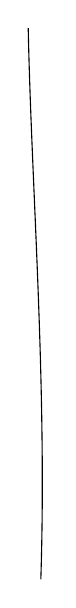
\begin{tikzpicture}\draw (0,0)..controls(.08,2.5)and(-.12,5)..(-.16,7);\end{tikzpicture}}}

À vrai dire, la démonstration via Mordell-Weil de l'unicité d'un $x$ \inserted{$\in X_K$} \unsure{qui} correspond à une classe donnée dans $H^1(\Gamma,\widehat\Pi_1(x_0))$, montre qu'on a unicité $=$ si on \deleted{\unsure{en donne}} \inserted{connaît} seulement l'élément correspondant à \deleted{\unsure{un}}
\[
\tag{34}(f_{x_0,x})_{\mathrm{ab}}\in H^1(\Gamma,\widehat\Pi_1(X,x_0)_{\mathrm{ab}}),
\]
et on peut déjà essayer de déterminer, par ``formules explicites'', les $(f_l)_{\mathrm{ab}}$ correspondant à des chemins $x_0\longrightarrow x$. On est réduit à regarder la $=$ question en remplaçant $X$ par une VA ou ext. d'icelle,

\margin{(C'est une question particulière, qui \unsure{bien plus intéressante|en plus intéressante} \illegible{2} \unsure{un problème} \unsure{variable} \unsure{en} $X$ \unsure{au-dessus de} $\unsure{\mathbb Q}$ \illegible{2}.)}

\scanpage{83}
\mspage{9}
par un tore --- pratiquement, par une ``jacobienne généralisée'' convenable de $X$.

Mais il faut se rappeler que pour une telle variété (p.ex. une courbe elliptique, ou la variété $G_m(\mathbb C)=\mathbb C^*$) l'opération de $\Gamma$ sur le groupoïde $\Pi_1(X_K)$ n'a plus rien de fidèle, donc pour ``repérer'' un $u\in\Gamma$, il ne suffit pas de connaître des invariants du type $g_l(u)$ \uline{relatifs à} \uline{ce même} $X$. Il faudra donc de façon essentielle introduire des ``paramètres de repérage'' pour $u$, en utilisant d'autres variétés algébriques déf sur $K$ --- la plus naturelle étant
\[
\tag{35}\unsure{U|\mathbf U}_{0,3}=\mathbb P^1\setminus\{0,1,\infty\}
\]
\figure{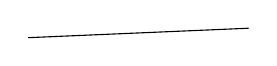
\begin{tikzpicture}\draw(0,0)--(2.8,.12);\end{tikzpicture}}
Faisant maintenant varier $X$, en considérant un morphisme de $K$-schémas
\[
\tag{36}f:X\mathbin{-}\unsure{X|Y}
\]
on déduit des morphismes de groupoïdes
\margin{82}

\scanpage{84}
\[
\tag{37}\diagram{\begin{tikzcd}[ampersand replacement=\&]\Pi_1(X)\arrow[r,no head,"f=\Pi_1(f)"]\&\Pi_1(Y)\end{tikzcd}}
\]
\[
\tag{38}\diagram{\begin{tikzcd}[ampersand replacement=\&]\widehat\Pi_1(X)\arrow[r,no head,"\widehat f=\widehat\Pi_1(f)"]\&\widehat\Pi_1(Y)\end{tikzcd}},
\]
dont le deuxième peut être déduit du premier par passage au groupoïde profini associé, mais peut aussi se décrire directement en termes purement schématiques, en termes \inserted{des morphismes} de schémas \deleted{\unsure{de|du}} $X\mathbin{-}Y$ sur le corps alg. clos $\mathbb C$. Par suite, (38) commute à l'action de $\unsure{\mathbf{\Gamma}|\Gamma}$,
\[
\tag{39}\widehat f({}^ul)={}^u(\widehat f(l))
\]
et si on se borne aux sous-groupoïdes induits sur $X_{\bar K},Y_{\bar K}$, \inserted{\unsure{d'où} ($\widehat\Pi_1(Y_{\bar K})$)}, ce dernier commute à l'action de $\Gamma=\operatorname{Gal}\bar K/K$. Si on se $=$ aux sous-groupoïdes induits $X_K$, d'où des $f_l(u),g_l(u)$ pour un chemin $l$ dans $X$ ou dans $Y$, on trouve aussitôt
\[
\tag{40}\left\{\begin{aligned}
\widehat f(f_l(u))&=f_{\widehat f(l)}(u)\\
\widehat f(g_l(u))&=g_{\widehat f(l)}(u).
\end{aligned}\right.
\]
\margin{Même formule \unsure{dans le cas} d'un $T$ $1$-connexe sur $X$ ($T$ esp. \unsure{topologique}), \unsure{donc} au-dessus de $Y$. On aura:
\[
\tag{40bis}g^{T/Y}_{y,x}(u)=\widehat f(g^{T/X}_{y,x}(u))
\]
\deleted{\unsure{d'où}}}
\margin{83}

\scanpage{85}
\mspage{10}
Un cas trivial intéressant est celui où $f$ est un isomorphisme --- et $=$ celui où $X=Y$, et où $f$ fait partie d'un groupe $\unsure{\mathcal G|G}$ de $K$-isomorphismes de $X$ --- alors on peut considérer $\Pi_1(X)$ et $\Pi_1(X_{\bar K}),\Pi_1(X_K)$ comme des groupoïdes où opère $\unsure{\mathcal G|G}$, et $\widehat\Pi_1(X)$ comme un groupoïde où opère $\unsure{\mathcal G|G}\times\unsure{\mathbf{\Gamma}|\Gamma}$, $\widehat\Pi_1(\unsure{\bar X|X}_{\bar K})$ comme un groupoïde sur lequel $\unsure{\mathcal G|G}\times\Gamma$ opère. Cette fois-ci le groupe n'opère pas trivialement sur les sommets de $\Pi_1(X_K)$, l'opération de $\Gamma$ est triviale, mais pas nécessairement celle de $\unsure{\mathcal G|G}$.

Si on se donne un pt $x_0\in X_K$ comme pt base, et un ens de sommets $I\subset X_K$ contenant $x_0$, l'opération de $\Gamma$ sur $\widehat\Pi_1(X,I)$ est connue quand on connaît son opération sur $\widehat\pi_1(X,x_0)$, et si de plus on connaît son opération sur les $\widehat\pi_1(X,x_0)$-torseurs à droite
\figure{\begin{tikzpicture}\draw(0,0)--(0,.65)--(1.3,.78)--(1.3,1);\end{tikzpicture}}
\[
\tag{41}\uline{\operatorname{Hom}}_{\widehat\Pi_1(X,I)}(x_0,x_i),\qquad i\in I.
\]
ou, ce qui revient au $=$, si on connaît les
\margin{84}

\scanpage{86}
\[
\tag{\unsure{41|42}}f_{l_i}(u)\qquad i\in I,\ u\in\Gamma
\]
où pour $\forall i\in I$, $l_i$ est un chemin dans $\Pi_1(X,x_i)$ de $x_0$ vers $x_i$, i.e. un élément de la partie ``discrète'' du torseur (41).

D'autre part, l'action de $\Gamma$ sur $\widehat\pi_1(X,x_0)$ est connue quand on connaît son action sur des générateurs $\lambda_j$ \inserted{($j\in J$)} de $\pi_1(X,x_0)$, i.e. si on connaît les
\[
\tag{43}f_{\lambda_j}(u)\quad\text{ou}\quad g_{\lambda_j}(u)\qquad j\in J,\ u\in\Gamma.
\]
\deleted{Mais cette} Les données (42)(43) suffisent donc à déterminer l'action de $\Gamma$ sur $\Pi_1(X,I)$ --- mais cette description, \deleted{à la} \deleted{\unsure{dis|dire}} s'il a l'avantage d'une économie, au moins en apparence, a le désavantage de se référer à des choix arbitraires, le pire étant le choix d'une \deleted{origine} \inserted{point-base} $x_0$ \deleted{à laquelle} \inserted{auquel} on est censé \unsure{tout} ramener --- ce qui semble artificiel, et à la longue je crois impraticable, \deleted{est} et tout particulièrement dans les situations impliquant un groupe de symétrie $\unsure{\mathcal G|G}$ comme ci-dessus, quand on a pris $I$ stable sous $\unsure{\mathcal G|G}$ ---
\margin{qu'il faut \unsure{exprimer} \unsure{linéairement|littéralement}, \unsure{resp.} \unsure{principes}, \unsure{décrit p.8!|c'est le pb!}}
\margin{85}

\scanpage{87}
\mspage{11}
alors que pratiquement jamais on ne pourra trouver un $x\in X_K$ \deleted{stable} \inserted{fixe} sous $\unsure{\mathcal G|G}$.
\figure{\begin{tikzpicture}\draw (0,0)--(1.4,0);\end{tikzpicture}}

Avant de donner un principe d'approche pour des calculs ``symétriques'', tenant compte de la présence d'un groupe $\unsure{\mathcal G|G}$ (cas d'une grande importance en pratique), je voudrais préciser la question des relations entre $\Pi_1(X,I)$ ($I$ partie finie de $X_K$) et $\Pi_1(U_{0,3})$, \deleted{et les} dans l'optique des opérations de $\Gamma$.
\inserted{Pour fixer les idées je suppose que $K$ est \deleted{de} fini sur $\mathbb Q$,} \inserted{et} Je prendrai le cas $X$ quasi-projective lisse géom.$^t$ connexe. Utilisant des th. du type Lefschetz, plus le résultat de \deleted{\unsure{Biel}} \unsure{Белый|Belyi}, on \deleted{\unsure{trouve|trouver}} doit pouvoir trouver deux hom de schémas sur $K$
\[
\tag{44}\diagram{\begin{tikzcd}[ampersand replacement=\&]
I \arrow[d,phantom,"{\rotatebox{-90}{$\subset$}}" description] \& \\
\unsure{\mathcal C|C} \arrow[r,hook,"i"] \arrow[d,"f"'] \& X \\
U_{0,3} \&
\end{tikzcd}}
\]
où $i$ induit un hom \uline{surjectif} sur les groupes fondamentaux, et où $f$ est
\margin{86}

\scanpage{88}
un morphisme fini étale. Ainsi $\Pi_1(X,I)$ apparaît comme quotient de $\Pi_1(C\deleted{\unsure{X}},I)$, donc $\widehat\Pi_1(X,I)$ quotient de $\widehat\Pi_1(C,I)$, et où $\Pi_1(C,I)$ apparaît comme un revêtement fini de $\Pi_1(U_{0,3},I)$ --- plus \deleted{précisément} \inserted{concrètement}, prenant le saturé $I'=f^{-1}f(I)=\unsure{f}^{-1}(I_0)$ de $I$, $\Pi_1(U_{0,3},I)$ est un sous-groupoïde \inserted{plein} de $\Pi_1(U_{0,3};I')$, qui lui est un rev. fini du groupoïde $\Pi_1(U_{0,3};I_0)$ --- et idem pour les complétés profinis. Ainsi, l'opération de $\Gamma$ sur $\widehat\Pi_1(X)$ est connue quand on connaît l'opération sur $\widehat\Pi_1(C,\widetilde I)$, qui est un rev. fini de $\widehat\Pi_1(U_{0,3};I_0)$. Si on connaît l'action de $\Gamma$ sur $\widehat\Pi_1(U_{0,3};I_0)$ lui-même, \deleted{\unsure{La} \unsure{on} doit pouvoir \inserted{\unsure{l'action|l'opération} sur $\widehat\Pi_1(U_{0,3})$}}
\margin{87}

\scanpage{89}
\mspage{12}
$\widehat\Pi_1(C,I')$ est déterminée \inserted{via (39) ou (40)}, car \unsure{l' pour|si pour} $x,y\in C$, l'application
\[
\operatorname{Hom}_{\widehat\Pi_1(C)}(x,y)\longrightarrow\operatorname{Hom}_{\widehat\Pi_1(U_{0,3})}(x,y)
\]
est injective!

\unsure{J'avais|J'ai} \unsure{pas} observé, \unsure{car|que} le saturé $I'$ de $I$ \inserted{dans $C$} n'est pas tjrs \deleted{fini} contenu dans \deleted{$\unsure{X}$} $C_K$ --- mais à vrai dire, rien ne m'obligeait à remplacer $I$ par $I'$ pour faire mon raisonnement: il reste vrai que la connaissance de l'action de $\Gamma$ sur sur $\widehat\Pi_1(U_{0,3},I_0)$ implique la connaissance de son action sur $\widehat\Pi_1(X,I)$. Mais il est vrai sûrement que l'étude des relations entre $\widehat\Pi_1(C;\deleted{\unsure{x}}I)$ et $\widehat\Pi_1(U_{0,3},I_0)$ en tant que groupoïdes à groupe d'opérations $\Gamma$, est facilité grandement en remplaçant $I$ par son saturé $I'$, $=$ si celui-ci n'est pas $\subset\deleted{X}C_K$. (Au besoin, si on est ennuyé par des sommets qui se balladent sous l'action de $\Gamma$, il n'y a
\margin{88}

\scanpage{90}
\margin{89}
qu'à remplacer $\Gamma$ par un sous-groupe ouvert convenable $\Gamma'$\ldots)

En $=$ temps, on entrevoit des conditions nécessaires draconiennes pour qu'un autom. \inserted{$\Theta$} du groupoïde $\Pi_1(U_{0,3};I_0)$, \unsure{laiss.$^t$|laiss.} \unsure{fixe|fixes} les sommets i.e. les pts de $I_0$, provienne d'un $u\in\Gamma$: il faut que pour $\forall$ revêtement \deleted{de $X$} étale $C$ de $U_{0,3}$, défini sur $K$, \inserted{prenant $I=f^{-1}(I_0)\subset C_K$ et \unsure{projetant|proj.} $I\to I_0$, \unsure{surj.}} \deleted{telle que} \deleted{l'action de} \deleted{\unsure{l'opération de}} \inserted{\unsure{que l'autom.}} $\Theta\deleted{_{\unsure{C_0}}}$ \deleted{de} $\Pi_1(U_{0,3},I_0)$ \deleted{provienne d'une action de} \inserted{soit ``compatible'' avec un autom.} $\Theta_C$ de $\Pi_1(C,I)$ \inserted{qui soit l'identité} \deleted{\unsure{qui soit ponctuel|qui soit ponctuellement}} \inserted{sur les sommets $I$} \deleted{par l'identi} (cet $\Theta_C$ sera alors unique). On trouve encore une condition, $=$ si $I-I_0$ n'est pas surjectif, et \deleted{en} \unsure{supposons|supposant} $=$ que $I_0\subset C_{0K}$ pour $\forall$ rev. étale de $U_{0,3}$, en exigeant qu'il existe une puissance $\Theta^n$ de $\Theta$ \inserted{($n\geq1$)} satisfaisant aux conditions précédentes, pour $I=f^{-1}(I_0)$.
\margin{(NB $C_0=U_{0,3}=P^1_{\mathbb C}\setminus\{0,1,\infty\}$)}
\margin{\unsure{Regarder} des \unsure{familles} \unsure{pour} $\unsure{C_0}$ \illegible{2} \deleted{\unsure{telles}} \unsure{conditions} \illegible{2}, quand on augmente $I_0$\ldots}

\scanpage{91}
\mspage{13}
Non seulement la condition de \deleted{\unsure{continuité}} ``prolongeabilité'' --- il vaut mieux dire d'``inductibilité'' --- sous la forme précisée, ou affaiblie (avec $\Theta$ remplacé par un $\Theta^n$), on trouve une condition supplémentaire, quand on a \inserted{de plus} un morphisme
\[
\widehat\Pi_1(C,I)\longrightarrow\widehat\Pi_1(X,I),
\]
que celui-ci passe au quotient --- ce qui s'exprime très exactement par la condition que pour \uline{un} $x_0\in I$, l'action de $\Gamma$ sur
\[
\widehat\pi_1(C,x_0)\subset\widehat\pi_1(U_{0,3},f(x_0))
\]
laisse stable le noyau de
\[
\widehat\pi_1(C,x_0)\longrightarrow\widehat\pi_1(X,x_0);
\]
alors ce sera vrai également pour tous les autres $x_i\in I$.

Il faut exprimer la possibilité de relever l'action de $\Theta$ à $\Pi_{\unsure{1|0}}(C,I)$. Notons à ce propos

\uline{Lemme} Soit $\mathcal C'-\mathcal C$ un hom de groupoïdes connexes, qui soit injectif sur les $\pi_1$, \deleted{\unsure{et}} de sorte que $\mathcal C'$ est équivalent à un revêtement de $\mathcal C$, mais on ne suppose pas que $\mathcal C'$ soit lui-$=$ un revêtement de $\mathcal C$, mais quand-même \unsure{que|pas}
\margin{90}

\scanpage{92}
l'homomorphisme canonique
\[
\tag{45}\mathcal C'\longrightarrow\widetilde{\mathcal C}^{\unsure{\prime|*}}.
\]
\inserted{vrai revêtement de $\mathcal C$, dont les sommets sont les $\pi_0$ des fibres de $\mathcal C'-\unsure{\mathcal C|\widetilde{\mathcal C}}$}
\deleted{\unsure{ce}} foncteur $\mathcal C'-\mathcal C$ est injectif, de sorte qu'on peut identifier $\mathcal C'$ à un sous-groupoïde plein de $\widetilde{\mathcal C}^{\unsure{\prime|*}}$, équivalent à $\widetilde{\mathcal C}^{\unsure{\prime|*}}$ par l'inclusion, où $\widetilde{\mathcal C}$ est un rev. fini de $\mathcal C$.

Soit $x'_0$ un sommet de $\mathcal C'$, $x_0$ son image dans $\widetilde{\mathcal C}$. Soit $\Theta$ un automorphisme de $\mathcal C$ qui fixe $x_0$, \deleted{alors s'}il \deleted{\unsure{y en a un de}} \inserted{revient au} $=$ de se donner un autom. de \deleted{$\unsure{\mathcal C}$} $\pi_1(\mathcal C,x_0)\overset{\mathrm{def}}{=}\pi_0$ (\unsure{abrég.}), et pour tout \inserted{sommet} $\deleted{\unsure{x}}x_i\in\operatorname{Ob}\mathcal C$, $x_i\ne x_0$, un automorphisme du $\pi_1(x_0)$-torseur à droite $H_{x_i,x_0}=\operatorname{Hom}_{\mathcal C}(x_0,x_i)$, compatible avec l'opération de $\Theta$ sur $\pi_0$. Ceci posé, pour que cette action se remonte en une action de $\widetilde{\mathcal C}$ qui fixe $x'_0$, il f. et s. que le sous-groupe $\pi'_0$ de $\pi_0$, image de \deleted{$\unsure{\pi_1}$}
\[
\pi_1(\widetilde{\mathcal C},x'_0)\hookrightarrow\pi_1(\mathcal C,x_0)=\pi_0,
\]
soit \uline{stable} par $\Theta$ --- l'action de $\Theta$ sur les fibres \inserted{$\widetilde{\mathcal C}_{x_i}$} de $\widetilde{\mathcal C}/\mathcal C$ est alors donnée par la formule
\[
\tag{45}\operatorname{Ob}\widetilde{\mathcal C}_{x_i}=H_{x_i,x_0}\wedge_{\pi_0}\underbrace{\pi_0/\pi'_0}_{\substack{\text{esp. hom}\\\text{des classes}\\\text{à droite, sur lequel}\\\pi_0\ \text{opère à g}}}
\]
par transport de structure à partir de son
\margin{91}

\scanpage{93}
\mspage{14}
action sur \deleted{$H_{x_i,x_0}$} le système $(\pi_0,H_{x_i,x_0},\underbrace{\pi_0/\pi'_0}_{\deleted{\unsure{esp}}})$ où on fait opérer $\Theta$ sur $\pi_0,H_{(x_i,x_0)}$ par son action sur $\mathcal C$, et sur $\pi_0/\pi'_0$ via l'action sur $\pi_0$, qui passe au quotient d'après la \deleted{hypothèse} \inserted{condition} \deleted{dite} envisagée. L'action \deleted{\unsure{prolong}} remontée \inserted{$\widetilde\Theta$ de $\Theta$} \deleted{est} sur $\widetilde{\mathcal C}$ est donc unique. Pour qu'il existe une action de $\Theta^{\unsure{*|\prime}}$ sur $\mathcal C'$ qui soit compatible avec $\mathcal C'-\mathcal C$, il f. et s. que la condition précédente soit satisfaite, et que \uline{de plus} $\operatorname{Ob}\mathcal C'\subset\operatorname{Ob}\mathcal C$ soit stable sous \deleted{cette} l'action de $\widetilde\Theta$.

Dans le cas où on ne suppose pas que l'on \deleted{dispose de} \inserted{donne} un $x'_0\in\operatorname{Ob}\mathcal C'$ dont on exige qu'il soit fixe par $\Theta$, on considère la fibre \inserted{$E_0=$} $\widetilde{\mathcal C}_{x_0}$, qui est un $\pi_0$-ensemble \deleted{\unsure{un}} homogène, et on note que les façons de remonter $\Theta$ en une action \inserted{$\widetilde\Theta$} dans $\widetilde{\mathcal C}$ correspondent \deleted{\unsure{aux}} exactement aux façons de remonter $\Theta$ en une action de $\widetilde\Theta_0$ sur $E_0$, \deleted{\unsure{comment|convenant}} soit compatible avec l'action sur $\pi_0$, i.e. satisfaisant
\margin{mais on suppose tjrs un $x_0$ fixe sous $\Theta$}
\figure{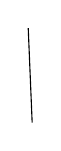
\begin{tikzpicture}\draw(0,0)--(-.05,1.2);\end{tikzpicture}}
\margin{Ceci vaut sans supposer $\widetilde{\mathcal C}$ connexe --- mais la traduction plus bas en termes de $\pi'_0\subset\pi_0$ dépend de la condition de connexité\ldots Cf plus bas le cas \unsure{où on a un|d'un} \unsure{s-grp|sous-groupoïde} plein $\unsure{\widetilde{\mathcal C}|\mathcal C}$ connexe.}
\[
\tag{46}\widetilde\Theta_0(g.x^{\deleted{\unsure{0}}\prime})=\Theta(g)\widetilde\Theta_0(x')
\]
--- \deleted{elle correspond} \inserted{une telle action est connue} quand on connaît, pour \uline{un} $x'_0$ fixé de $E_0=\operatorname{Ob}\widetilde{\mathcal C}_{x_0}$, son transformé par $\widetilde\Theta_0$, la formule (46) donnant tous les autres \inserted{$\widetilde\Theta_0(x')$, \deleted{\unsure{puisque}} $\unsure{\forall}x'\in E_0$}. En termes
\margin{92}
